\mfpicnumber{1}

\opengraphsfile{Transformations}

\setcounter{footnote}{0}

\label{Transformations}

Theorems \ref{linearabsvaluegraphs}, \ref{standardformgraph}, \ref{linearmononialgraphs},  \ref{linearlaurentlgraphs}, \ref{linearrootgraphs} and \ref{linearrationalpowergraphs} all describe ways in which the graph of a function can changed, or `transformed' to obtain the graph of a related function. The results and  proofs  of each of these theorems are virtually identical, and with the language of function composition, we can see better why.  

\smallskip

Consider, for instance, Theorem \ref{linearrationalpowergraphs}, in which we describe how to transform the graph of $f(x) = x^r$ to  $F(x) = a(bx-h)^r +k$.  We may think of $F$ as being build up from $f$ by composing $f$ with linear functions.  Specifically, if we let $i(x) = bx-h$, then $(f\circ i)(x) = f(i(x)) = f(bx-h) = (bx-h)^r$.  If, additionally, we let and $j(x) = ax+k$, then $(j \circ (f \circ i))(x) = j( (f \circ i)(x)) = j((bx-h)^r) = a(bx-h)^r+k = F(x)$.  Hence, we can view $F = j \circ f \circ i$.  

\smallskip

In this section, our goal is to generalize the aforementioned theorems to the graphs of \textit{all} functions.  Along the way, you'll see some very familiar arguments, but, additionally, we hope this section affords the reader an opportunity to not only see \textit{how} these transformations work they way they do, but \textit{why}.

\smallskip

Our motivational example for the results in this section is the graph of $y = f(x)$ below.  While we could formulate an expression for $f(x)$ as a piecewise-defined function consisting of linear and constant parts, we wish to focus more on the geometry here.  That being said, we do record some of the function values - the `key points' if you will - to track through each transformation.


\begin{center}

\begin{tabular}{m{2.5in} m{2.5in}}

\begin{mfpic}[15]{-1}{6}{-1}{6}
\tlabel[cc](-1,1){\scriptsize $(0,1)$}
\tlabel[cc](2,3.5){\scriptsize $(2,3)$}
\tlabel[cc](4,2.5){\scriptsize $(4,3)$}
\tlabel[cc](5,5.5){\scriptsize $(5,5)$}
\tlabel[cc](6,-0.5){\scriptsize $x$}
\tlabel[cc](0.5,6){\scriptsize $y$}
\tcaption{\scriptsize $y=f(x)$}
\axes
\xmarks{1,2,3,4,5}
\ymarks{1,2,3,4,5}
\tlpointsep{4pt}
\axislabels {x}{{\scriptsize $1$} 1, {\scriptsize $2$} 2, {\scriptsize $3$} 3, {\scriptsize $4$} 4, {\scriptsize $5$} 5}
\axislabels {y}{{\scriptsize $2$} 2, {\scriptsize $3$} 3, {\scriptsize $4$} 4, {\scriptsize $5$} 5}
\penwd{1.25pt}
\polyline{(0,1), (2,3), (4,3), (5,5)}
\point[4pt]{(0,1), (2,3), (4,3), (5,5)}
\end{mfpic}


&

\[ \begin{array}{|c||c|c|}  

\hline

 x & (x,f(x)) & f(x)  \\ \hline
0  & (0,1)& 1  \\  \hline
2 & (2,3) & 3  \\  \hline
4 & (4,3) & 3  \\  \hline
5 & (5,5) & 5 \\  \hline

\end{array} \] 



\end{tabular}

\end{center}

\subsection{Vertical and Horizontal Shifts}
\label{shifts}

Suppose we wished to graph $g(x) = f(x) + 2$.  From a procedural point of view,  we start with an input $x$ to the function $f$ and we obtain the output $f(x)$.  The function $g$ takes the output $f(x)$ and adds $2$ to it.  Using the sample values for $f$ from the table above we can create a table of values for $g$ below, hence generating points on the graph of $g$.


\[ \begin{array}{|c||c|c|c|c|}  

\hline

 x & (x,f(x)) & f(x) & g(x)=f(x)+2 & (x, g(x)) \\ \hline
0  & (0,1)& 1 & 1+2 = 3 &(0, 3) \\  \hline
2 & (2,3) & 3 & 3 + 2 =  5 &(2,5) \\  \hline
4 & (4,3) & 3 & 3 + 2 =  5 &(4, 5) \\  \hline
5 & (5,5) & 5 & 5+2 =  7 &( 5 ,7) \\  \hline

\end{array} \] 

In general,  if $(a,b)$ is on the graph of $y=f(x)$, then $f(a) = b$. Hence, $g(a) = f(a) +2 = b+2$, so the point $(a,b+2)$ is on the graph of $g$. In other words, to obtain the graph of $g$, we add $2$ to the $y$-coordinate of each point on the graph of $f$.  

\smallskip

Geometrically, adding $2$ to the $y$-coordinate of a point moves the point $2$ units above its previous location.  Adding $2$ to every $y$-coordinate on a graph \textit{en masse} is moves or `shifts'  the entire graph of $f$  up $2$ units.  Notice that the graph retains the same basic shape as before, it is just $2$ units above its original location.  In other words, we connect the four `key points' we moved in the same manner in which they were connected before.  
\[ \begin{array}{ccc}


\begin{mfpic}[15]{-1}{6}{-1}{8}

\tlabel[cc](-1,1){\scriptsize $(0,1)$}
\tlabel[cc](2,3.5){\scriptsize $(2,3)$}
\tlabel[cc](4,2.5){\scriptsize $(4,3)$}
\tlabel[cc](5,5.5){\scriptsize $(5,5)$}
\tlabel[cc](6,-0.5){\scriptsize $x$}
\tlabel[cc](0.5,8){\scriptsize $y$}
\tcaption{\scriptsize $y=f(x)$}
\axes
\xmarks{1,2,3,4,5}
\ymarks{1,2,3,4,5,6,7}
\tlpointsep{4pt}
\axislabels {x}{{\scriptsize $1$} 1, {\scriptsize $2$} 2, {\scriptsize $3$} 3, {\scriptsize $4$} 4, {\scriptsize $5$} 5}
\axislabels {y}{{\scriptsize $2$} 2,  {\scriptsize $3$} 3, {\scriptsize $4$} 4, {\scriptsize $5$} 5, {\scriptsize $6$} 6, {\scriptsize $7$} 7}
\penwd{1.25pt}
\polyline{(0,1), (2,3), (4,3), (5,5)}
\point[4pt]{(0,1), (2,3), (4,3), (5,5)}
\end{mfpic}

&

\stackrel{\stackrel{\mbox{\scriptsize shift up $2$ units}}{\xrightarrow{\hspace{1in}}}}{\mbox{ \scriptsize add $2$ to each $y$-coordinate}} 

& 

\begin{mfpic}[15]{-1}{6}{-1}{8}

\tlabel[cc](-1,3){\scriptsize $(0,3)$}
\tlabel[cc](2,5.5){\scriptsize $(2,5)$}
\tlabel[cc](4,4.5){\scriptsize $(4,5)$}
\tlabel[cc](5,7.5){\scriptsize $(5,7)$}
\tlabel[cc](6,-0.5){\scriptsize $x$}
\tlabel[cc](0.5,8){\scriptsize $y$}
\tcaption{\scriptsize $y=g(x) = f(x)+2$}
\axes
\xmarks{1,2,3,4,5}
\ymarks{1,2,3,4,5,6,7}
\tlpointsep{4pt}
\axislabels {x}{{\scriptsize $1$} 1, {\scriptsize $2$} 2, {\scriptsize $3$} 3, {\scriptsize $4$} 4, {\scriptsize $5$} 5}
\axislabels {y}{{\scriptsize $1$} 1,{\scriptsize $2$} 2,  {\scriptsize $4$} 4, {\scriptsize $5$} 5, {\scriptsize $6$} 6, {\scriptsize $7$} 7}
\penwd{1.25pt}
\polyline{(0,3), (2,5), (4,5), (5,7)}
\point[4pt]{(0,3), (2,5), (4,5), (5,7)}
\end{mfpic} \end{array}\]
 
You'll note that the domain of $f$ and the domain of $g$ are the same, namely $[0,5]$, but that the range of $f$ is $[1,5]$ while the range of $g$ is $[3,7]$.  In general, shifting a function vertically like this will leave the domain unchanged, but could very well affect the range.  

\smallskip

You can easily imagine what would happen if we wanted to graph the function $j(x) = f(x) - 2$.  Instead of adding $2$ to each of the $y$-coordinates on the graph of $f$, we'd be subtracting $2$.  Geometrically, we would be moving the graph down $2$ units.  We leave it to the reader to verify that the domain of $j$ is the same as $f$, but the range of $j$ is $[-1,3]$.  In general, we have:

\smallskip

\colorbox{ResultColor}{\bbm

%\smallskip

\begin{thm} \label{vshifts} \textbf{Vertical Shifts.}\index{graph ! vertical shift} Suppose $f$ is a function and $k$ is a real number. 

To graph $F(x) = f(x) + k$,  add $k$ to each of the $y$-coordinates of the points on the graph of $y=f(x)$.

\textbf{NOTE:}  This results in a vertical shift up $k$ units if $k > 0$ or down $k$ units if $k< 0$.


\end{thm}

\ebm}

\smallskip

To prove Theorem \ref{vshifts}, we first note that $f$ and $F$ have the same domain (why?)  Let $c$ be an element in the domain of $F$ and, hence, the domain of $f$.  The fact that $f$ and $F$ are \textit{functions} guarantees  there is \textit{exactly one} point on each of their  graphs corresponding to $x=c$.  On $y=f(x)$, this point is $(c, f(c))$;  on $y = F(x)$, this point is  $(c, F(c)) = (c, f(c)+k)$.  This sets up a nice correspondence between the two graphs and shows that each of the points on the graph of $F$ can be obtained to by adding $k$ to each of the $y$-coordinates of the corresponding point on the graph  of $f$.  This  proves  Theorem \ref{vshifts}.   In the language of `inputs' and `outputs', Theorem \ref{vshifts} says adding to the \textit{output} of a function causes the graph to shift \textit{vertically}. 
 
\smallskip

Keeping with the graph of $y=f(x)$ above, suppose we wanted to graph $g(x) = f(x+2)$.  In other words, we are looking to see what happens when we add $2$ to the input of the function. Let's try to generate a table of values of $g$ based on those we know for $f$.  We quickly find that we run into some difficulties. For instance, when we substitute $x=4$ into the formula $g(x)=f(x+2)$, we are asked to find $f(4+2)=f(6)$ which doesn't exist because the domain of $f$ is only $[0,5]$.  The same thing happens when we attempt to find $g(5)$. 

\[ \begin{array}{|c||c|c|c|c|}  

\hline

x & (x,f(x)) & f(x)& g(x)=f(x+2) & (x, g(x)) \\ \hline
0  & (0,1)& 1 & g(0) = f(0+2) = f(2) = 3   &(0, 3) \\  \hline
2 & (2,3) & 3 & g(2) = f(2+2) = f(4) = 3  &(2,3) \\  \hline
4 & (4,3) & 3 &  g(4) = f(4+2) = f(6) = ? &  \\  \hline
5 & (5,5) & 5 & g(5) = f(5+2) = f(7) = ?  &  \\  \hline

\end{array} \]

 What we need here is a new strategy.  We know, for instance, $f(0) = 1$.  To determine the corresponding point on the graph of $g$, we need to figure out what value of $x$ we must substitute into $g(x) = f(x+2)$ so that the quantity $x+2$, works out to be $0$.  Solving $x+2=0$ gives $x=-2$, and $g(-2) = f((-2)+2) = f(0) = 1$ so  $(-2,1)$ on the graph of $g$.  To use the fact $f(2) = 3$, we set $x+2 = 2$ to get $x=0$. Substituting gives $g(0) = f(0+2) = f(2) = 3$. Continuing in this fashion, we produce the table below.
 
 
\[ \begin{array}{|r||c|c|c|}  

\hline

x & x+2 & g(x)=f(x+2) & (x, g(x)) \\ \hline
-2 & 0 & g(-2)=f(-2+2) = f(0) = 1   &(-2, 1) \\  \hline
0 &  2 &  g(0)=f(0+2) = f(2) = 3  &(0,3) \\  \hline
2 & 4  & g(2)=f(2+2) = f(4) = 3 &  (2,3)\\  \hline
3 & 5 & g(3)=f(3+2) = f(5) = 5  & (3,5) \\  \hline

\end{array} \]

In summary, the points $(0,1)$, $(2,3)$, $(4,3)$ and $(5,5)$ on the graph of $y=f(x)$ give rise to the points  $(-2,1)$, $(0,3)$, $(2,3)$ and $(3,5)$ on the graph of $y=g(x)$, respectively.  In general, if $(a,b)$ is on the graph of $y=f(x)$, then $f(a) = b$.  Solving $x+2 = a$ gives $x = a-2$ so that $g(a-2) = f((a-2)+2) = f(a) = b$.  As such, $(a-2,b)$ is on the graph of $y=g(x)$. The point $(a-2,b)$ is exactly $2$ units to the \emph{left} of the point $(a,b)$ so the graph of $y=g(x)$ is obtained by shifting the graph $y=f(x)$ to the left $2$ units, as pictured below.

\[\begin{array}{ccc}

\begin{mfpic}[15]{-3}{6}{-1}{6}
\tlabel[cc](-1,1){\scriptsize $(0,1)$}
\tlabel[cc](2,3.5){\scriptsize $(2,3)$}
\tlabel[cc](4,2.5){\scriptsize $(4,3)$}
\tlabel[cc](5,5.5){\scriptsize $(5,5)$}
\tlabel[cc](6,-0.5){\scriptsize $x$}
\tlabel[cc](0.5,6){\scriptsize $y$}
\tcaption{\scriptsize $y=f(x)$}
\axes
\xmarks{-2,-1, 1,2,3,4,5}
\ymarks{1,2,3,4,5}
\tlpointsep{4pt}
\axislabels {x}{{\scriptsize $-2 \hspace{7pt}$} -2, {\scriptsize $-1\hspace{7pt}$} -1,{\scriptsize $1$} 1, {\scriptsize $2$} 2, {\scriptsize $3$} 3, {\scriptsize $4$} 4, {\scriptsize $5$} 5}
\axislabels {y}{{\scriptsize $2$} 2, {\scriptsize $3$} 3, {\scriptsize $4$} 4, {\scriptsize $5$} 5}
\penwd{1.25pt}
\polyline{(0,1), (2,3), (4,3), (5,5)}
\point[4pt]{(0,1), (2,3), (4,3), (5,5)}
\end{mfpic} 

&

\stackrel{\stackrel{\mbox{\scriptsize shift left $2$ units}}{\xrightarrow{\hspace{1in}}}}{\mbox{ \scriptsize subtract $2$ from each $x$-coordinate}} 

& 

\begin{mfpic}[15]{-3}{6}{-1}{6}
\tlabel[cc](-3,1){\scriptsize $(-2,1)$}
\tlabel[cc](-1,3){\scriptsize $(0,3)$}
\tlabel[cc](2,2.5){\scriptsize $(2,3)$}
\tlabel[cc](3,5.5){\scriptsize $(3,5)$}
\tlabel[cc](6,-0.5){\scriptsize $x$}
\tlabel[cc](0.5,6){\scriptsize $y$}
\tcaption{\scriptsize $y=g(x)=f(x+2)$}
\axes
\xmarks{-2,-1, 1,2,3,4,5}
\ymarks{1,2,3,4,5}
\tlpointsep{4pt}
\axislabels {x}{{\scriptsize $-2 \hspace{7pt}$} -2, {\scriptsize $-1\hspace{7pt}$} -1,{\scriptsize $1$} 1, {\scriptsize $2$} 2, {\scriptsize $3$} 3, {\scriptsize $4$} 4, {\scriptsize $5$} 5}
\axislabels {y}{{\scriptsize $1$} 1, {\scriptsize $2$} 2, {\scriptsize $4$} 4, {\scriptsize $5$} 5}
\penwd{1.25pt}
\polyline{(-2,1), (0,3), (2,3), (3,5)}
\point[4pt]{(-2,1), (0,3), (2,3), (3,5)}
\end{mfpic}

\end{array}\]

Note that while the ranges of $f$ and $g$ are the same, the domain of $g$ is $[-2,3]$ whereas the domain of $f$ is $[0,5]$.  In general, when we shift the graph horizontally, the range will remain the same, but the domain could change.  If we set out to graph $j(x) = f(x-2)$, we would find ourselves \textit{adding} $2$ to all of the $x$ values of the points on the graph of $y=f(x)$ to effect a shift to the \emph{right} $2$ units. Generalizing these notions produces the following result.

\smallskip

\colorbox{ResultColor}{\bbm

%\smallskip

\begin{thm} \label{hshifts}\textbf{Horizontal Shifts.}\index{graph ! horizontal shift}  Suppose $f$ is a function and $h$ is a real number. 

To graph $F(x) = f(x-h)$,  add $h$ to each of the $x$-coordinates of the points on the graph of $y=f(x)$.

\textbf{NOTE:}  This results in a horizontal shift right $h$ units if $h > 0$ or left $h$ units if $h< 0$.

\end{thm}

\ebm}

\smallskip

To prove Theorem \ref{hshifts}, we first note the domains of $f$ and $F$ may be different.   If $c$ is in the domain of $f$, then the only number we know for sure is in the domain of $F$ is  $c+h$, since $F(c+h) = f((c+h)-h) = f(c)$.  This sets up a nice correspondence between the domain of $f$ and the domain of $F$ which spills over to a correspondence between their graphs,  The point $(c, f(c))$ is the one and only point on the graph of $y = f(x)$ corresponding to $x=c$ just as the point $(c+h, F(c+h)) = (c+h, f(c))$ is the one and only point on the graph of $y = F(x)$ corresponding to $x=c+h$.  This correspondence shows we may obtain the graph of $F$ by adding $h$ to each $x$-coordinate of each point on the graph of $f$, which establishes the theorem. In words, Theorem \ref{hshifts} says that subtracting from the  \textit{input} to a function amounts to shifting the graph \textit{horizontally}. 

\smallskip

 Theorems \ref{vshifts} and \ref{hshifts} present a theme which will run common throughout the section:  changes to the \textit{outputs} from a function result in some kind of \textit{vertical change};  changes to the \textit{inputs} to a function result in some kind of \textit{horizontal} change.  We demonstrate  Theorems \ref{vshifts} and \ref{hshifts} in the example below.
 
 \begin{ex} \label{shiftex}  Use Theorems  \ref{vshifts} and \ref{hshifts} to answer the questions below.  Check your answers using a graphing utility where appropriate.
 
 \begin{enumerate}
 
 \item  Suppose $(-1,3)$ is on the graph of $y = f(x)$.  Find a point on the graph of:
 
 \begin{multicols}{3}
 
 \begin{enumerate}
 
 \item $y = f(x)+5$
 
 \item $y = f(x+5)$
 
 \item  $f(x-7)+4$
 
 \end{enumerate}
 
 \end{multicols}
 
 \item  Find a formula for a function $g(t)$ whose graph is the same as $f(t) = |t|-2t$ but is shifted:
 
 \begin{multicols}{2}
 
 \begin{enumerate}
 
 \item to the right $4$ units.
 
 \item down $2$ units.
 
 \end{enumerate}
 
 \end{multicols}
 
 \item Predict how the graph of $F(x) = \dfrac{(x-2)^{\frac{2}{3}}}{x}$ relates to the graph of $f(x) = \dfrac{x^{\frac{2}{3}}}{x+2}$. 
 
\item  Below on the left is the graph of $y = f(x)$.  Use it to sketch the graph of

  \begin{multicols}{3}
 
 \begin{enumerate}
 
 \item $F(x) = f(x-2)$
 
 \item $F(x)= f(x)+1$
 
  \item $F(x)= f(x+1)-2$
 
 \end{enumerate}
 
 \end{multicols}
 
 \item  Below on the right is the graph of $y = g(x)$.  Write $g(x)$ in terms of $f(x)$ and vice-versa.
 
\begin{center}

\begin{multicols}{2}

\begin{mfpic}[15]{-3}{6}{-1}{5}
\axes
\tlabel[cc](6,-0.5){\scriptsize $x$}
\tlabel[cc](0.5,5){\scriptsize $y$}
\xmarks{-2, -1, 0, 1, 2, 3, 4,5}
\ymarks{-1, 0, 1, 2, 3,4}
\tcaption{\scriptsize $y = f(x)$}
\tlpointsep{4pt}
\scriptsize
\tlabel[cc](-2.25, -0.5){$(-2,0)$}
\tlabel[cc](-1, 3){$(0,3)$}
\tlabel[cc](2, 4.5){$(2,4)$}
\tlabel[cc](4, 2.5){$(4,3)$}
\axislabels {x}{{$1$} 1, {$2$} 2,  {$3$} 3,{$4$} 4, {$5$} 5}
\axislabels {y}{{$2$} 2,{$1$} 1,{$4$} 4}
\normalsize
\penwd{1.25pt}
\function{-2, 4, 0.1}{(x+2)*(6-x)/4}
\point[4pt]{(-2,0), (2,4), (0,3)}
\pointfillfalse
\point[4pt]{(4,3)}
\end{mfpic}



\begin{mfpic}[15]{-3}{6}{-1}{5}
\axes
\tlabel[cc](6,-0.5){\scriptsize $x$}
\tlabel[cc](0.5,5){\scriptsize $y$}
\xmarks{-2, -1, 0, 1, 2, 3, 4,5}
\ymarks{-1, 0, 1, 2, 3,4}
\tcaption{\scriptsize $y =g(x)$}
\tlpointsep{4pt}
\scriptsize
\tlabel[cc](-1.75, -1.5 ){$(-1.5,-1)$}
\gclear \tlabelrect(-0.5, 2){$(0.5,2)$}
\tlabel[cc](2.5, 3.5){$(2.5,3)$}
\tlabel[cc](4.5, 1.5){$(4.5,2)$}
\axislabels {x}{{$1$} 1, {$2$} 2,  {$3$} 3,{$4$} 4, {$5$} 5}
\axislabels {y}{{$4$} 4,{$3$} 3}
\normalsize
\penwd{1.25pt}
\function{-1.5, 4.5, 0.1}{((x+1.5)*(6.5-x)/4)-1}
\point[4pt]{(-1.5,-1), (2.5,3), (0.5,2)}
\pointfillfalse
\point[4pt]{(4.5,2)}
\end{mfpic}

 
 
\end{multicols}
 
\end{center}
 
 \end{enumerate}
 
 \newpage
 
 {\bf Solution.}
 
 \begin{enumerate}
 
 \item 
  
 \begin{enumerate}  
 
 \item To apply Theorem \ref{vshifts}, we identify $f(x)+5 = f(x)+k$  so $k = 5$.  Hence, we add $5$ to the $y$-coordinate of $(-1,3)$  and get  $(-1,3+5) = (-1,8)$.  To check our answer note since $(-1,3)$ is on the graph of $f$ this means $f(-1) = 3$.  Substituting  $x=-1$ into the formula $y = f(x)+5$, we get $y = f(-1)+5 = 3+5 = 8$.  Hence, $(-1,8)$ is on the graph of $f(x)+5$.
 
 \item We note that $f(x+5)$ can be written as $f(x-(-5)) = f(x-h)$ so we apply Theorem \ref{hshifts} with $h=-5$.  Adding $-5$ to (subtracting $5$ from) the $x$-coordinate of  $(-1,3)$ gives $(-1+(-5), 3) = (-6,3)$.  To check our answer,  since $(-1,3)$ is on the graph of $f$, $f(-1) = 3$.  Substituting $x=-6$ into $y=f(x+5)$ gives $y=f(-6+5)=f(-1)=3$, proving $(-6,3)$ is on the graph of $y=f(x+5)$.
 
 \item Note that the expression $f(x-7)+4$ differs from $f(x)$ in \textit{two} ways indicating \text{two} different transformations. In situations like this, its best if we handle each transformation in turn, starting with the graph of  $y=f(x)$ and `building up' to the graph of $y = f(x-7)+4$.  
 
 \smallskip
 
 We choose to work from the `inside' (argument) out and use Theorem \ref{hshifts} to first get a point on the graph of $y=f(x-7) = f(x-h)$. Identifying $h=7$, we add $7$ to the $x$-coordinate of $(-1,3)$ to get $(-1+7,3) = (6,3)$.  Hence, $(6,3)$ is a point on the graph of $y = f(x-7)$.  
 
 \smallskip
 
 Next, we apply Theorem \ref{vshifts} to graph $y = f(x-7)+4$ starting with $y=f(x-7)$.  Viewing $f(x-7)+4 = f(x-7)+k$, we identify $k=4$ and add  $4$ to the $y$-coordinate of $(6,3)$ to get $(6,3+4) = (6,7)$.  To check, we note that if we substitute $x=6$ into $y = f(x-7)+4$, we get $y=f(6-7)+4 = f(-1)+4 = 3+4 =7$.
 
 \end{enumerate}
 
 \item  Here the independent variable is $t$ instead of $x$ which doesn't affect the geometry in any way since our convention is the independent variable is used to label the horizontal axis and the dependent variable is used to label the vertical axis.  
 
 \begin{enumerate}
 
 \item  Per Theorem \ref{hshifts}, the graph of $g(t) = f(t-4) = |t-4|-2(t-4) = |t-4|-2t+8$ should be the graph of $f(t) = |t|-2t$ shifted to the right $4$ units. Our check is below on the left.
  
 \item Per Theorem \ref{vshifts},  the graph of $g(t) = f(t)+(-2) = |t|-2t+(-2) = |t|-2t-2$ should be the graph of  $f(t) = |t|-2t$ shifted down $2$ units. Our check is below on the right.
 
  \end{enumerate}
 
\begin{center}

\begin{tabular}{cc}

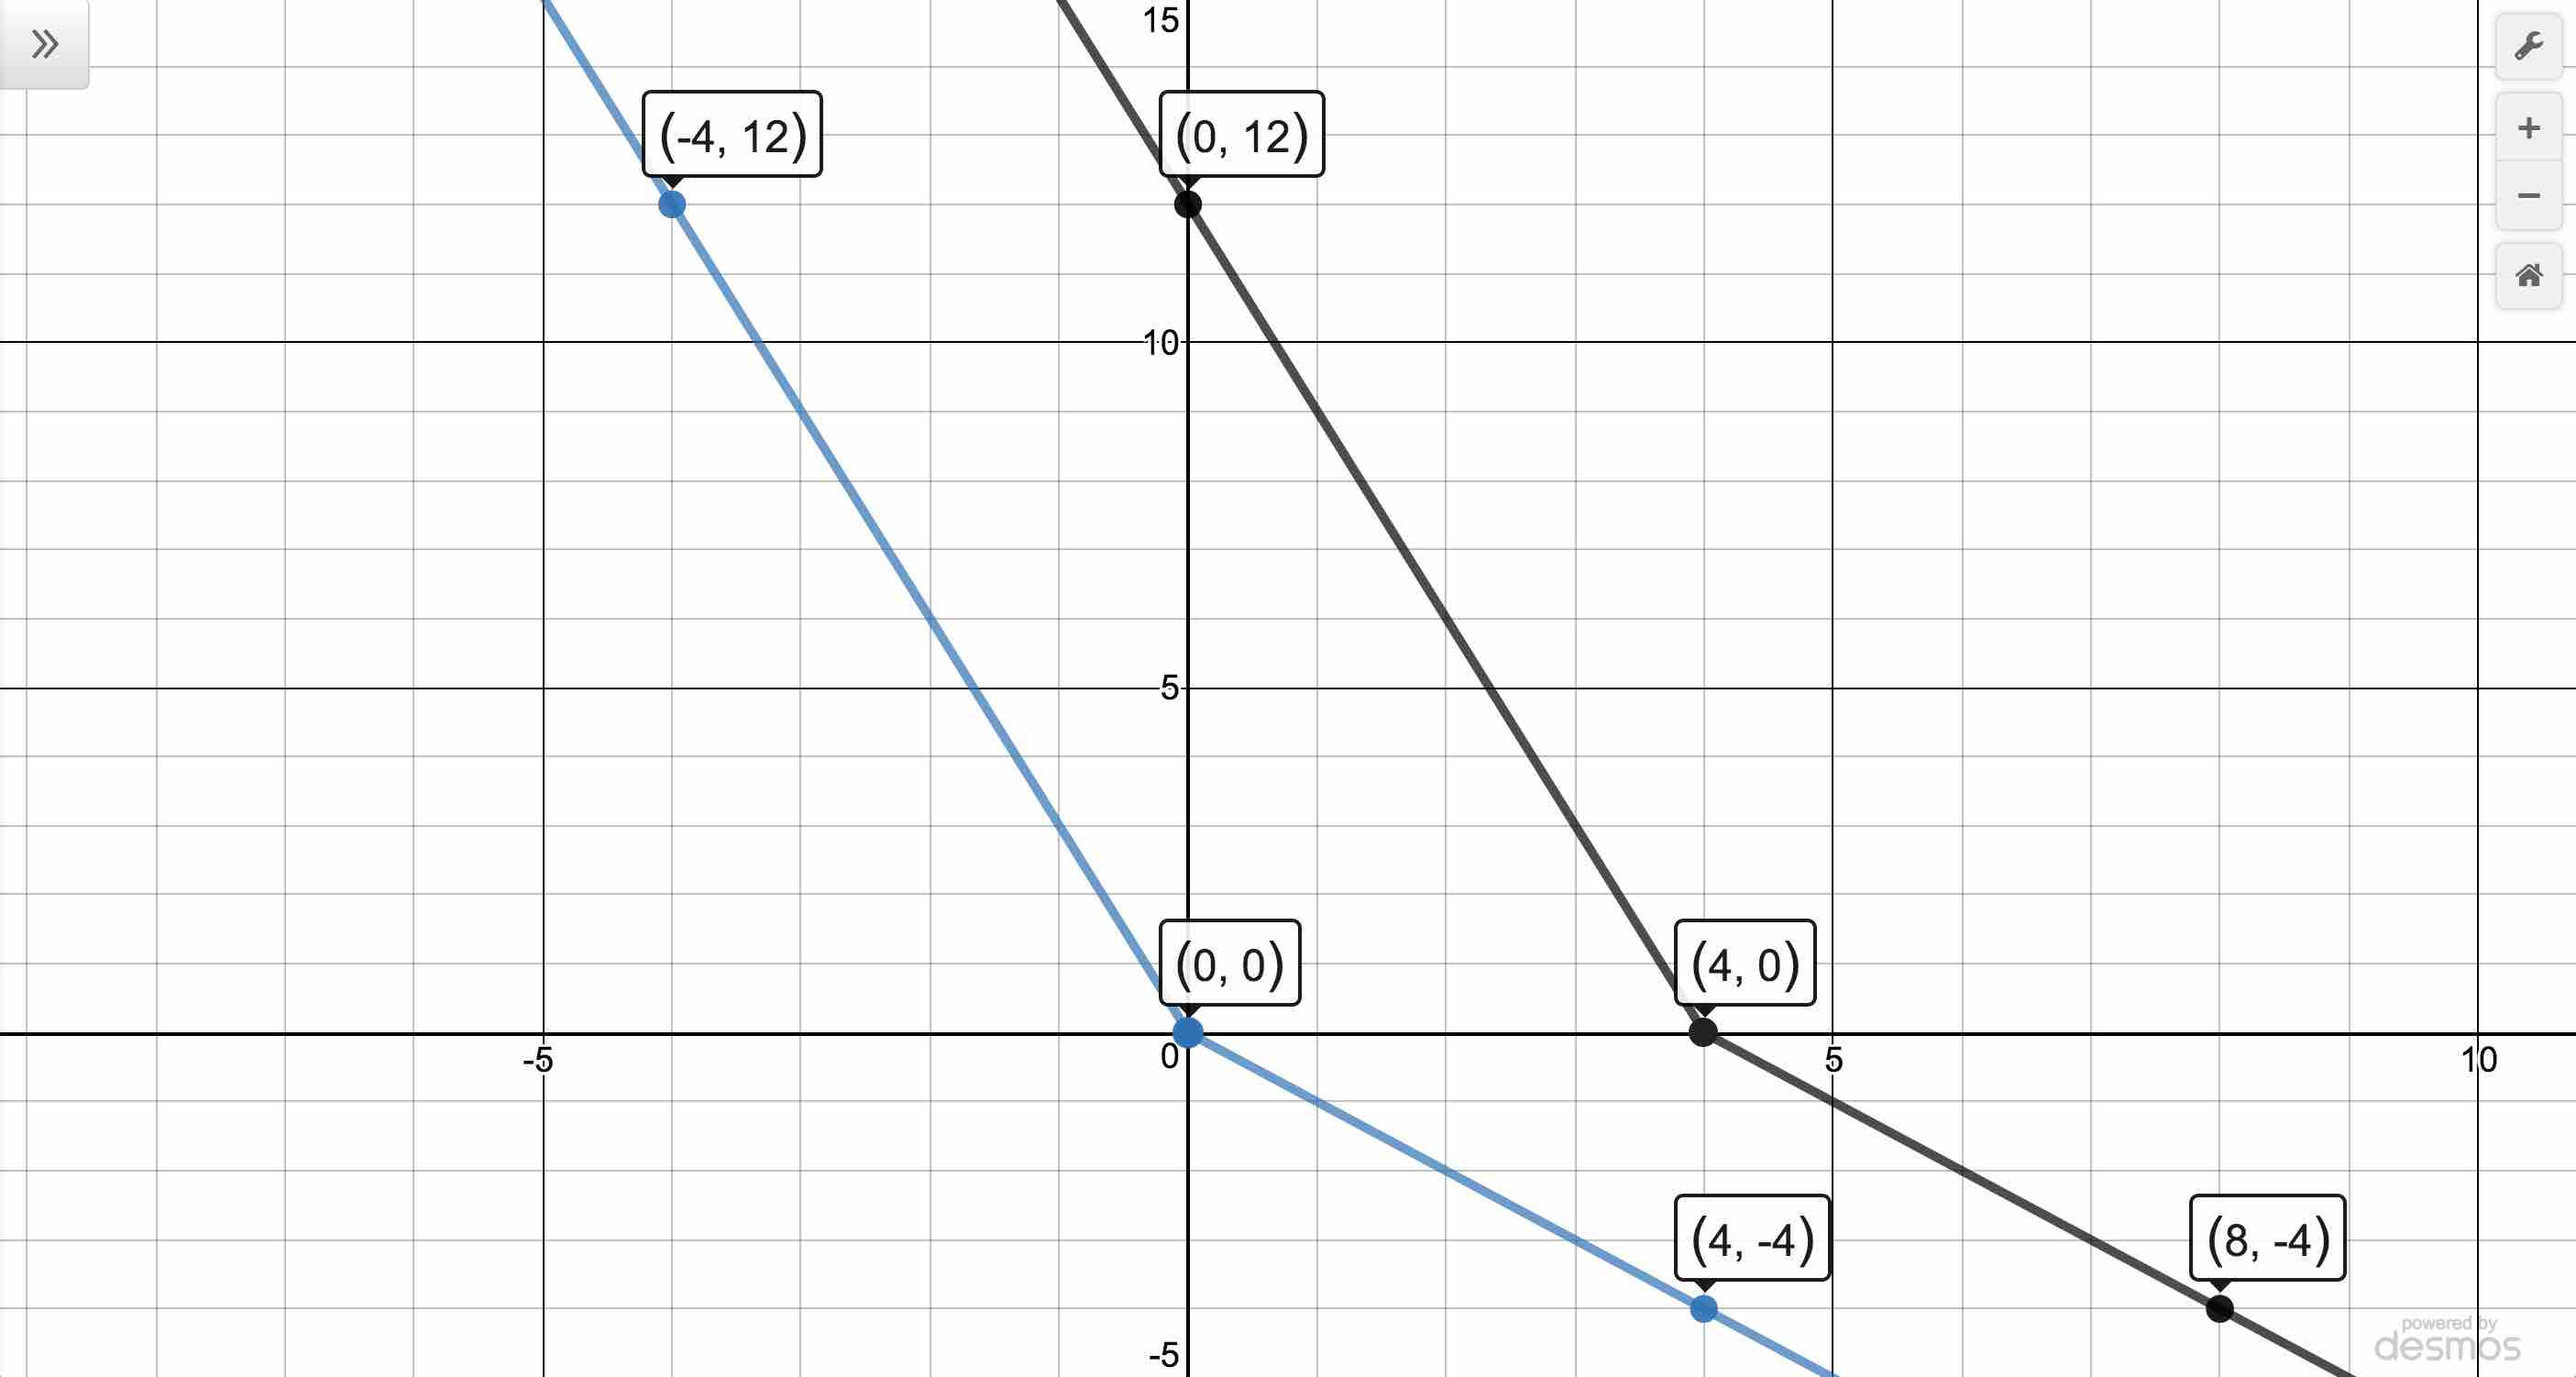
\includegraphics[width=3in]{./TransformationsGraphics/TransformationsEx01a.jpg} & 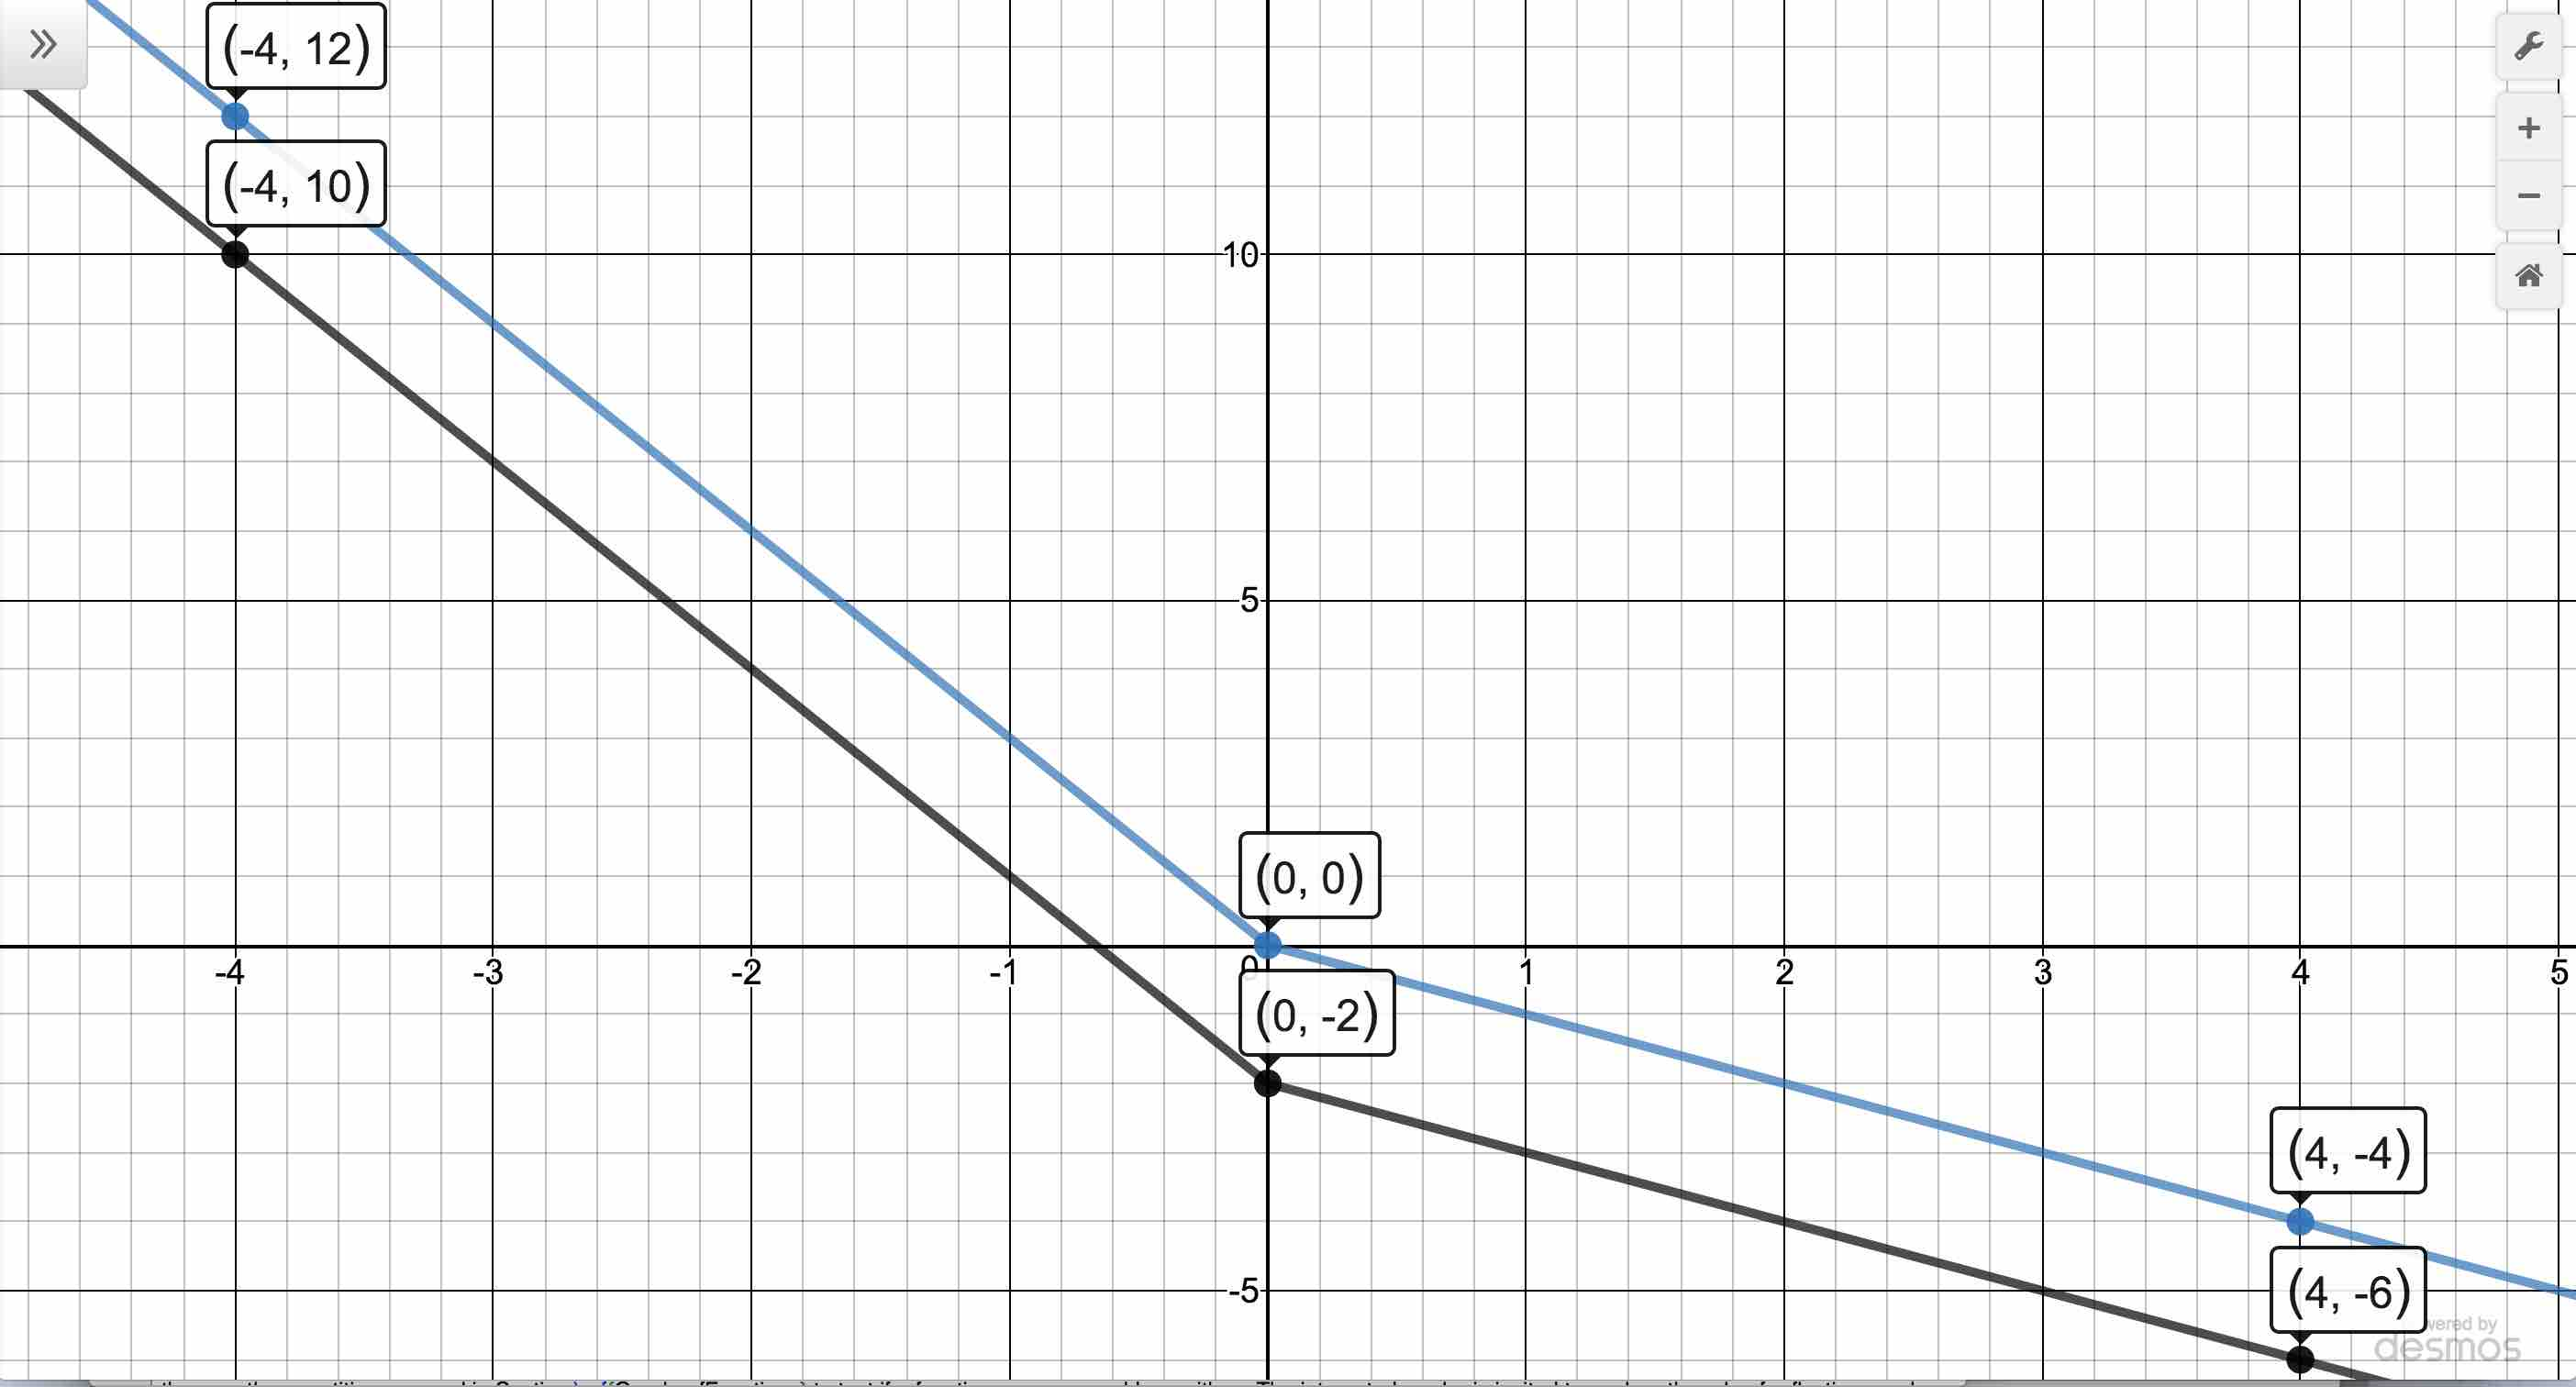
\includegraphics[width=3in]{./TransformationsGraphics/TransformationsEx01b.jpg} \\

$y =  |t|-2t$ (lighter color)  and $y = |t-4|-2t+8$  &  $y =  |t|-2t$ (lighter color) and $y =  |t|-2t-2$ \\

\end{tabular}

\end{center} 

\item  Comparing \textit{formulas}, it appears as if $F(x) = f(x-2)$.  We check: \[ f(x-2) = \dfrac{(x-2)^{\frac{2}{3}}}{(x-2)+2} = \dfrac{(x-2)^{\frac{2}{3}}}{x} = F(x),\]  so, per Theorem \ref{hshifts},  the graph of $y = F(x)$ should be the graph of $y=f(x)$ but shifted to the right $2$ units. We graph both functions below to confirm our answer.

\begin{center}

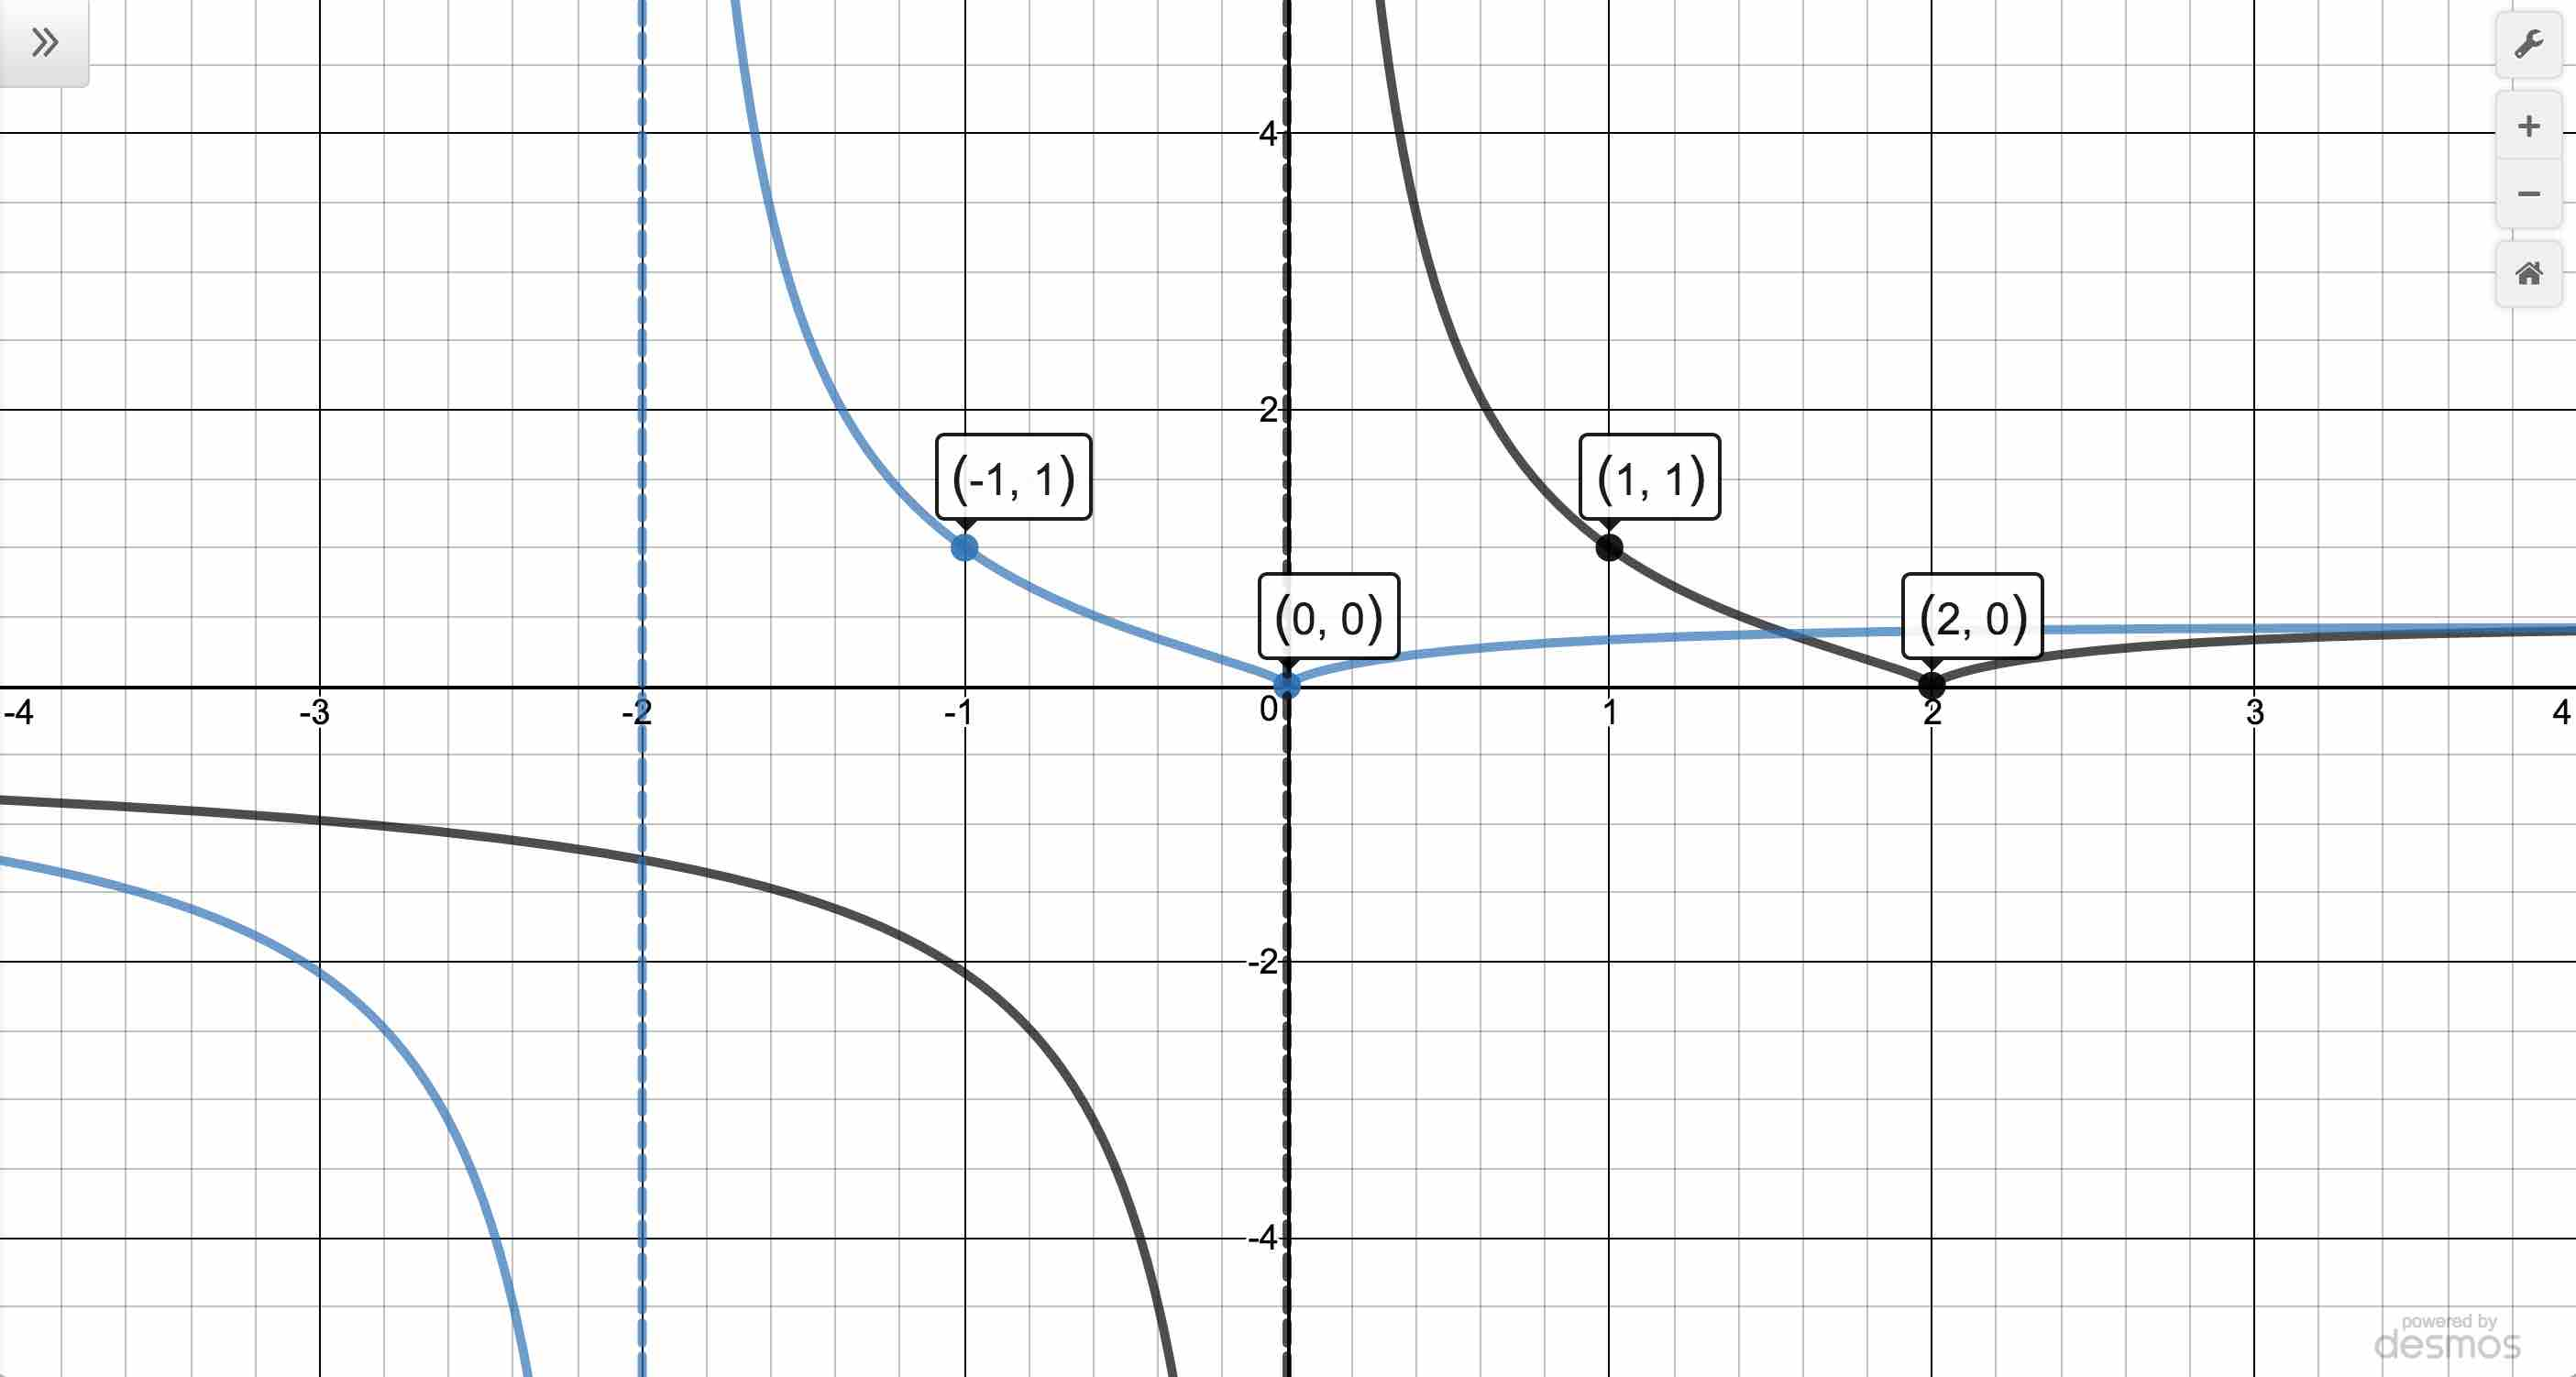
\includegraphics[width=4in]{./TransformationsGraphics/TransformationsEx01c.jpg}

$y = \dfrac{x^{\frac{2}{3}}}{x+2}$ (lighter color) and $y = \dfrac{(x-2)^{\frac{2}{3}}}{x}$ 

\end{center}

\item 

\begin{enumerate}  

\item  We recognize  $F(x) = f(x-2) =f(x-h)$. With $h=2$, Theorem \ref{hshifts} tells us to add $2$ to each of the $x$-coordinates of the points on the graph of $f$, moving the graph of $f$ to the \textit{right} two units.

\[\begin{array}{ccc}

\begin{mfpic}[15]{-3}{8}{-1}{5}
\axes
\tlabel[cc](8,-0.5){\scriptsize $x$}
\tlabel[cc](0.5,5){\scriptsize $y$}
\xmarks{-2, -1, 0, 1, 2, 3, 4,5,6,7}
\ymarks{0, 1, 2, 3,4}
\tcaption{\scriptsize $y = f(x)$}
\tlpointsep{4pt}
\scriptsize
\tlabel[cc](-2.25, -0.5){$(-2,0)$}
\tlabel[cc](-1, 3){$(0,3)$}
\tlabel[cc](2, 4.5){$(2,4)$}
\tlabel[cc](4, 2.5){$(4,3)$}
\axislabels {x}{{$1$} 1, {$2$} 2,  {$3$} 3,{$4$} 4,{$5$} 5,{$6$} 6,{$7$} 7}
\axislabels {y}{{$2$} 2,{$1$} 1,{$4$} 4}
\normalsize
\penwd{1.25pt}
\function{-2, 4, 0.1}{(x+2)*(6-x)/4}
\point[4pt]{(-2,0), (2,4), (0,3)}
\pointfillfalse
\point[4pt]{(4,3)}
\end{mfpic}

&

\stackrel{\stackrel{\mbox{\scriptsize shift right  $2$ units}}{\xrightarrow{\hspace{1in}}}}{\mbox{ \scriptsize add $2$ to each $x$-coordinate}} 

& 

\begin{mfpic}[15]{-3}{8}{-1}{5}
\axes
\tlabel[cc](8,-0.5){\scriptsize $x$}
\tlabel[cc](0.5,5){\scriptsize $y$}
\xmarks{-2, -1, 0, 1, 2, 3, 4,5,6,7}
\ymarks{0, 1, 2, 3,4}
\tcaption{\scriptsize $y = F(x) = f(x-2)$}
\tlpointsep{4pt}
\scriptsize
\gclear \tlabelrect(0, -0.5){$(0,0)$}
\tlabel[cc](1, 3){$(2,3)$}
\tlabel[cc](4, 4.5){$(4,4)$}
\tlabel[cc](6, 2.5){$(6,3)$}
\axislabels {x}{{$1$} 1, {$2$} 2,  {$3$} 3,{$4$} 4,{$5$} 5,{$6$} 6,{$7$} 7}
\axislabels {y}{{$2$} 2,{$1$} 1,{$4$} 4,{$3$} 3}
\normalsize
\penwd{1.25pt}
\function{0, 6, 0.1}{(x)*(8-x)/4}
\point[4pt]{(0,0), (4,4), (2,3)}
\pointfillfalse
\point[4pt]{(6,3)}
\end{mfpic}

\end{array}\]

We can check our answer by showing each ordered pair $(x,y)$ listed on our final graph satisfies the equation $y = f(x-2)$.  Starting with $(0,0)$, we substitute $x=0$ into $y=f(x-2)$ and get $y = f(0-2) = f(-2)$.  Since $(-2,0)$ is on the graph of $f$, we know $f(-2) = 0$.  Hence, $y = f(0-2) = f(-2) = 0$, showing the point $(0,0)$ is on the graph of $y=f(x-2)$.  We invite the reader to check the remaining points.

\item  We have $F(x) = f(x)+1 = f(x)+k$ where $k=1$, so  Theorem \ref{vshifts} tells us to move the graph of $f$ \textit{up} $1$ unit by adding $1$ to each of the $y$-coordinates of the points on the graph of $f$.

\[\begin{array}{ccc}

\begin{mfpic}[15]{-3}{6}{-1}{6}
\axes
\tlabel[cc](6,-0.5){\scriptsize $x$}
\tlabel[cc](0.5,6){\scriptsize $y$}
\xmarks{-2, -1, 0, 1, 2, 3, 4,5}
\ymarks{0, 1, 2, 3,4,5}
\tcaption{\scriptsize $y = f(x)$}
\tlpointsep{4pt}
\scriptsize
\tlabel[cc](-2.25, -0.5){$(-2,0)$}
\tlabel[cc](-1, 3){$(0,3)$}
\tlabel[cc](2, 4.5){$(2,4)$}
\tlabel[cc](4, 2.5){$(4,3)$}
\axislabels {x}{{$1$} 1, {$2$} 2,  {$3$} 3,{$4$} 4, {$5$} 5}
\axislabels {y}{{$2$} 2,{$1$} 1,{$4$} 4,{$5$} 5}
\normalsize
\penwd{1.25pt}
\function{-2, 4, 0.1}{(x+2)*(6-x)/4}
\point[4pt]{(-2,0), (2,4), (0,3)}
\pointfillfalse
\point[4pt]{(4,3)}
\end{mfpic}

&

\stackrel{\stackrel{\mbox{\scriptsize shift up $1$ unit}}{\xrightarrow{\hspace{1in}}}}{\mbox{ \scriptsize add $1$ to each $y$-coordinate}} 

& 

\begin{mfpic}[15]{-3}{6}{-1}{6}
\axes
\tlabel[cc](6,-0.5){\scriptsize $x$}
\tlabel[cc](0.5,6){\scriptsize $y$}
\xmarks{-2, -1, 0, 1, 2, 3, 4,5}
\ymarks{0, 1, 2, 3,4,5}
\tcaption{\scriptsize $y = F(x) =  f(x)+1$}
\tlpointsep{4pt}
\scriptsize
\tlabel[cc](-2.25, 0.5){$(-2,1)$}
\tlabel[cc](-1, 4){$(0,4)$}
\tlabel[cc](2, 5.5){$(2,5)$}
\tlabel[cc](4, 3.5){$(4,4)$}
\axislabels {x}{{$1$} 1, {$2$} 2,  {$3$} 3,{$4$} 4, {$5$} 5}
\axislabels {y}{{$2$} 2,{$1$} 1,{$3$} 3,{$5$} 5}
\normalsize
\penwd{1.25pt}
\function{-2, 4, 0.1}{1+(x+2)*(6-x)/4}
\point[4pt]{(-2,1), (2,5), (0,4)}
\pointfillfalse
\point[4pt]{(4,4)}
\end{mfpic}

\end{array}\]

To check our answer, we proceed as above.  Starting with the point $(-2,1)$, we substitute  $x=-2$ into $y=f(-2)+1$ to get $y = f(-2)+1$.  Since $(-2,0)$ is on the graph of $f$, we know $f(-2) = 0$.  Hence, $y = f(-2)+1 =0+1 = 1$.  This proves $(-2,1)$ is on the graph of $y=f(x)+1$.  We encourage the reader to check the remaining points in kind. 

\item  We are asked to graph $F(x) = f(x+1) -2$.  As above, when we have more than one modification to do, we work from the inside out and build up to $F(x)=f(x+1)-2$  from $f(x)$ in stages.   First, we apply Theorem \ref{hshifts} to graph $y=f(x+1)$ from $y=f(x)$.   Rewriting $f(x+1) = f(x-(-1))$, we identify $h=-1$,  so we add  $-1$ to (subtract $1$ from) each of the $x$-coordinates on the graph of $f$, shifting it to the \textit{left} $1$ unit.

\[\begin{array}{ccc}

\begin{mfpic}[15]{-4}{6}{-1}{5}
\axes
\tlabel[cc](6,-0.5){\scriptsize $x$}
\tlabel[cc](0.5,5){\scriptsize $y$}
\xmarks{-3,-2, -1, 0, 1, 2, 3, 4,5}
\ymarks{0, 1, 2, 3,4}
\tcaption{\scriptsize $y = f(x)$}
\tlpointsep{4pt}
\scriptsize
\tlabel[cc](-2.25, -0.5){$(-2,0)$}
\tlabel[cc](-1, 3){$(0,3)$}
\tlabel[cc](2, 4.5){$(2,4)$}
\tlabel[cc](4, 2.5){$(4,3)$}
\axislabels {x}{{$1$} 1, {$2$} 2,  {$3$} 3,{$4$} 4, {$5$} 5}
\axislabels {y}{{$2$} 2,{$1$} 1,{$4$} 4}
\normalsize
\penwd{1.25pt}
\function{-2, 4, 0.1}{(x+2)*(6-x)/4}
\point[4pt]{(-2,0), (2,4), (0,3)}
\pointfillfalse
\point[4pt]{(4,3)}
\end{mfpic}

&

\stackrel{\stackrel{\mbox{\scriptsize shift left $1$ unit}}{\xrightarrow{\hspace{1in}}}}{\mbox{ \scriptsize subtract $1$ from each $x$-coordinate}} 

& 

\begin{mfpic}[15]{-4}{6}{-1}{5}
\axes
\tlabel[cc](6,-0.5){\scriptsize $x$}
\tlabel[cc](0.5,5){\scriptsize $y$}
\xmarks{-3,-2, -1, 0, 1, 2, 3, 4,5}
\ymarks{0, 1, 2, 3,4}
\tcaption{\scriptsize $y  = f(x+1)$}
\tlpointsep{4pt}
\scriptsize
\tlabel[cc](-3.25, -0.5){$(-3,0)$}
\tlabel[cc](-2, 3){$(1,3)$}
\tlabel[cc](1, 4.5){$(1,4)$}
\tlabel[cc](3, 2.5){$(3,3)$}
\axislabels {x}{{$1$} 1, {$2$} 2,  {$3$} 3,{$4$} 4, {$5$} 5, {\scriptsize $-1\hspace{7pt}$} -1}
\axislabels {y}{{$2$} 2,{$1$} 1,{$4$} 4}
\normalsize
\penwd{1.25pt}
\function{-3, 3, 0.1}{(x+3)*(5-x)/4}
\point[4pt]{(-3,0), (1,4), (-1,3)}
\pointfillfalse
\point[4pt]{(3,3)}
\end{mfpic}

\end{array}\]

Next, we apply Theorem \ref{vshifts}  to graph $y = f(x+1)-2$ starting with the graph of $y=f(x+1)$.  Writing $f(x+1)-2=f(x+1)+(-2) = f(x+1)+k$, we identify $k=-2$ so  Theorem \ref{vshifts} instructs us to add $-2$ to (subtract $2$ from) each of the $y$-coordinates on the graph of $y = f(x+1)$, thereby shifting the graph \textit{down} two units.

\[\begin{array}{ccc}

\begin{mfpic}[15]{-4}{6}{-3}{5}
\axes
\tlabel[cc](6,-0.5){\scriptsize $x$}
\tlabel[cc](0.5,5){\scriptsize $y$}
\xmarks{-3,-2, -1, 0, 1, 2, 3, 4,5}
\ymarks{-2, -1, 0, 1, 2, 3,4}
\tcaption{\scriptsize $y = f(x+1)$}
\tlpointsep{4pt}
\scriptsize
\tlabel[cc](-3.25, -0.5){$(-3,0)$}
\tlabel[cc](-2, 3){$(1,3)$}
\tlabel[cc](1, 4.5){$(1,4)$}
\tlabel[cc](3, 2.5){$(3,1)$}
\axislabels {x}{{$1$} 1, {$2$} 2,  {$3$} 3,{$4$} 4, {$5$} 5, {\scriptsize $-1\hspace{7pt}$} -1}
\axislabels {y}{{$2$} 2,{$1$} 1,{$4$} 4,{$-1$} -1,{$-2$} -2, ,{$3$} 3}
\normalsize
\penwd{1.25pt}
\function{-3, 3, 0.1}{(x+3)*(5-x)/4}
\point[4pt]{(-3,0), (1,4), (-1,3)}
\pointfillfalse
\point[4pt]{(3,3)}
\end{mfpic}

&

\stackrel{\stackrel{\mbox{\scriptsize shift down $2$ units}}{\xrightarrow{\hspace{1in}}}}{\mbox{ \scriptsize subtract $2$ from each $y$-coordinate}} 

& 


\begin{mfpic}[15]{-4}{6}{-3}{5}
\axes
\tlabel[cc](6,-0.5){\scriptsize $x$}
\tlabel[cc](0.5,5){\scriptsize $y$}
\xmarks{-3,-2, -1, 0, 1, 2, 3, 4,5}
\ymarks{-2, -1, 0, 1, 2, 3,4}
\tcaption{\scriptsize $y = f(x+1)-2=F(x)$}
\tlpointsep{4pt}
\scriptsize
\tlabel[cc](-3.25, -2.5){$(-3,-2)$}
\tlabel[cc](-2, 1){$(1,1)$}
\tlabel[cc](1, 2.5){$(1,2)$}
\tlabel[cc](3, 0.5){$(3,2)$}
\axislabels {x}{{$1$} 1, {$2$} 2,  {$3$} 3,{$4$} 4, {$5$} 5, {\scriptsize $-1\hspace{7pt}$} -1}
\axislabels {y}{{$2$} 2,{$1$} 1,{$4$} 4,{$-1$} -1,{$-2$} -2, ,{$3$} 3}
\normalsize
\penwd{1.25pt}
\function{-3, 3, 0.1}{((x+3)*(5-x)/4)-2}
\point[4pt]{(-3,-2), (1,2), (-1,1)}
\pointfillfalse
\point[4pt]{(3,1)}
\end{mfpic}

\end{array}\]

To check, we start with the point $(-3, -2)$.  We find when we substitute $x=-3$ into the equation $y=f(x+1)-2$ we get $y = f(-3+1)-2 = f(-2)-2$.  Since $(-2,0)$ is on the graph of $f$, we know $f(-2) =0$, so  $y = f(-3+1)-2 = f(-2)-2 = 0 - 2 = -2$.  This proves $(-3,-2)$ is on the graph of $y=f(x+1)-2$.  We leave the checks of the remaining points to the reader.

\end{enumerate}

\item  To write $g(x)$ in terms of $f(x)$, we note that based on points which are labeled, it appears as if the graph of $g$ can be obtained from the graph of $f$ by shifting the graph of $f$ to the right $0.5$ units and down $1$ unit.  

\smallskip

Per Theorems \ref{hshifts} and \ref{vshifts}, $g(x)$ must take the form $g(x) = f(x-h)+k$.  Since the horizontal shift is to the \textit{right} $0.5$ units, $h = 0.5$ and since the vertical shift is \textit{down} $1$ unit, $k = -1$.   Hence, we get $g(x) = f(x-0.5)-1$.  

\smallskip

We can check our answer by working through both transformations, in sequence, as in the previous example.   To write $f(x)$ in terms of $g(x)$, we need to reverse the process - that is, we need to shift the graph of $g$ \textit{left} one half of a unit and \textit{up} one unit.   Theorems \ref{hshifts} and \ref{vshifts} suggest the formula $f(x) = g(x+0.5)+1$.  We leave it to the reader to check. \qed
  
 \end{enumerate}
 
 \end{ex}
 
\subsection{Reflections about the Coordinate Axes}

We now turn our attention to reflections. We know from Section \ref{AppCartesianPlane} that to reflect a point $(x,y)$ across the $x$-axis, we replace $y$ with $-y$.  If $(x,y)$ is on the graph of $f$, then $y=f(x)$, so replacing $y$ with $-y$ is the same as replacing $f(x)$ with $-f(x)$.  Hence, the graph of $y=-f(x)$ is the graph of $f$ reflected across the $x$-axis.  Similarly, the graph of $y=f(-x)$ is the graph of $y = f(x)$ reflected across the $y$-axis.\footnote{The expressions $-f(x)$ and $f(-x)$ should look familiar - they are the quantities we used in Section \ref{GraphsofPolynomials} to determine if a function was even, odd or neither.  We explore impact of symmetry on reflections in Exercise \ref{SymmetryandReflectionsExercise}.}   

\smallskip

\colorbox{ResultColor}{\bbm

%\smallskip

\begin{thm} \label{reflections}\index{graph ! reflection about an axis}\index{reflection ! of a function graph}\textbf{Reflections.}  Suppose $f$ is a function. 

  To graph $F(x)=-f(x)$,  multiply each of the $y$-coordinates of the points on the graph of $y=f(x)$ by $-1$.

\textbf{NOTE:}  This results in a reflection across the $x$-axis.

To graph $F(x)=f(-x)$,  multiply each of the $x$-coordinates of the points on the graph of $y=f(x)$ by $-1$.

\textbf{NOTE:}  This results in a reflection across the $y$-axis.


\end{thm}

\ebm}

\smallskip

The proof of Theorem \ref{reflections} follows in much the same way as the proofs of Theorems \ref{vshifts} and \ref{hshifts}.  If $c$ is an element of the domain of $f$ and $F(x) = -f(x)$,  then the point $(c, f(c))$ corresponds to the point $(c, F(c)) = (c,-f(c))$.  Comparing the corresponding points $(c, f(c))$ and $(c, -f(c))$, we see they only difference is the $y$-coordinates are the exact opposite - indicating they are mirror-images across the $x$-axis.  Similarly, if $c$ is an element in the domain of $f$, then $c$ corresponds to the element $-c$ in the domain of $F(x) = f(-x)$ since $F(-c) = f(-(-c)) = f(c)$. Hence, the corresponding points here are $(c, f(c))$ and $(-c, F(-c)) = (-c, f(c))$.  Comparing $(c, f(c))$ with $(-c, f(c))$, we see they are reflections about the $y$-axis.

\smallskip

Using the  language of inputs and outputs, Theorem \ref{reflections} says that multiplying the \textit{outputs} from a function by $-1$ reflects its graph across the \textit{horizontal} axis, while multiplying the \textit{inputs} to a function by $-1$ reflects the graph across the \textit{vertical} axis.

\smallskip

Applying Theorem \ref{reflections} to the graph of $y=f(x)$ given at the beginning of the section, we can graph $y=-f(x)$ by reflecting the graph of $f$ about the $x$-axis.

\[ \begin{array}{|c||c|c|c|c|}  

\hline

 x & (x,f(x)) & f(x) & g(x)=-f(x) & (x, g(x)) \\ \hline
0  & (0,1)& 1 & -1 &(0, -1) \\  \hline
2 & (2,3) & 3 &  -3 &(2,-3) \\  \hline
4 & (4,3) & 3 &  -3&(4, -3) \\  \hline
5 & (5,5) & 5 &  -5 &( 5 ,-5) \\  \hline

\end{array} \] 

\[ \begin{array}{ccc}

\begin{mfpic}[14]{-1}{6}{-6}{6}
\tlabel[cc](-1,1){\scriptsize $(0,1)$}
\tlabel[cc](2,3.5){\scriptsize $(2,3)$}
\tlabel[cc](4,2.5){\scriptsize $(4,3)$}
\tlabel[cc](5,5.5){\scriptsize $(5,5)$}
\tlabel[cc](6,-0.5){\scriptsize $x$}
\tlabel[cc](0.5,6){\scriptsize $y$}
\tcaption{\scriptsize $y=f(x)$}
\axes
\xmarks{1,2,3,4,5}
\ymarks{-1,-2,-3,-4,-5,1,2,3,4,5}
\tlpointsep{4pt}
\axislabels {x}{{\scriptsize $1$} 1, {\scriptsize $2$} 2, {\scriptsize $3$} 3, {\scriptsize $4$} 4, {\scriptsize $5$} 5}
\axislabels {y}{{\scriptsize $-1$} -1,{\scriptsize $-2$} -2, {\scriptsize $-3$} -3, {\scriptsize $-4$} -4, {\scriptsize $-5$} -5, {\scriptsize $2$} 2, {\scriptsize $3$} 3, {\scriptsize $4$} 4, {\scriptsize $5$} 5}
\penwd{1.25pt}
\polyline{(0,1), (2,3), (4,3), (5,5)}
\point[4pt]{(0,1), (2,3), (4,3), (5,5)}
\end{mfpic}

&

\stackrel{\stackrel{\mbox{\scriptsize reflect across $x$-axis}}{\xrightarrow{\hspace{1in}}}}{\mbox{ \scriptsize multiply each $y$-coordinate by $-1$}} 

&

\begin{mfpic}[14]{-1}{6}{-6}{6}
\tlabel[cc](-1.25,-1){\scriptsize $(0,-1)$}
\tlabel[cc](2,-3.5){\scriptsize $(2,-3)$}
\tlabel[cc](4,-2.5){\scriptsize $(4,-3)$}
\tlabel[cc](5,-5.5){\scriptsize $(5,-5)$}
\tlabel[cc](6,-0.5){\scriptsize $x$}
\tlabel[cc](0.5,6){\scriptsize $y$}
\tcaption{\scriptsize $y=-f(x)$}
\axes
\xmarks{1,2,3,4,5}
\ymarks{-1,-2,-3,-4,-5,1,2,3,4,5}
\tlpointsep{4pt}
\axislabels {x}{{\scriptsize $1$} 1, {\scriptsize $2$} 2, {\scriptsize $3$} 3, {\scriptsize $4$} 4, {\scriptsize $5$} 5}
\axislabels {y}{{\scriptsize $-2$} -2, {\scriptsize $-3$} -3, {\scriptsize $-4$} -4, {\scriptsize $-5$} -5,{\scriptsize $1$} 1,{\scriptsize $2$} 2, {\scriptsize $3$} 3, {\scriptsize $4$} 4, {\scriptsize $5$} 5}
\penwd{1.25pt}
\polyline{(0,-1), (2,-3), (4,-3), (5,-5)}
\point[4pt]{(0,-1), (2,-3), (4,-3), (5,-5)}
\end{mfpic}

\end{array}\]

By reflecting the graph of $f$ across the $y$-axis, we obtain the graph of $y=f(-x)$.

\[ \begin{array}{|r||c|c|c|}  

\hline

x & -x & g(x)=f(-x) & (x, g(x)) \\ \hline
0 & 0 & g(0)=f(-(-0)) = f(0) = 1   &(0, 1) \\  \hline
-2 & 2 &  g(-2)=f(-(-2)) = f(2) = 3  &(-2,3) \\  \hline
-4 & 4 & g(-4)=f(-(-4)) = f(4) = 3 &  (-4,3)\\  \hline
-5 & 5 & g(-5)=f(-(-5)) = f(5) = 5  & (-5,5) \\  \hline

\end{array} \]

\[ \begin{array}{ccc}

\begin{mfpic}[13]{-6}{6}{-1}{6}
\tlabel[cc](-1,1){\scriptsize $(0,1)$}
\tlabel[cc](2,3.5){\scriptsize $(2,3)$}
\tlabel[cc](4,2.5){\scriptsize $(4,3)$}
\tlabel[cc](5,5.5){\scriptsize $(5,5)$}
\tlabel[cc](6,-0.5){\scriptsize $x$}
\tlabel[cc](0.5,6){\scriptsize $y$}
\tcaption{\scriptsize $y=f(x)$}
\axes
\xmarks{-1,-2,-3,-4,-5,1,2,3,4,5}
\ymarks{1,2,3,4,5}
\tlpointsep{4pt}
\axislabels {x}{{\scriptsize $-1 \hspace{7pt}$} -1, {\scriptsize $-2\hspace{7pt}$} -2, {\scriptsize $-3\hspace{7pt}$} -3, {\scriptsize $-4\hspace{7pt}$} -4, {\scriptsize $-5\hspace{7pt}$} -5, {\scriptsize $1$} 1, {\scriptsize $2$} 2, {\scriptsize $3$} 3, {\scriptsize $4$} 4, {\scriptsize $5$} 5}
\axislabels {y}{{\scriptsize $2$} 2, {\scriptsize $3$} 3, {\scriptsize $4$} 4, {\scriptsize $5$} 5}
\penwd{1.25pt}
\polyline{(0,1), (2,3), (4,3), (5,5)}
\point[4pt]{(0,1), (2,3), (4,3), (5,5)}
\end{mfpic}

&

\stackrel{\stackrel{\mbox{\scriptsize reflect across $y$-axis}}{\xrightarrow{\hspace{1in}}}}{\mbox{ \scriptsize multiply each $x$-coordinate by $-1$}} 

&

\begin{mfpic}[13]{-6}{6}{-1}{6}
\tlabel[cc](1,1){\scriptsize $(0,1)$}
\tlabel[cc](-2,3.5){\scriptsize $(-2,3)$}
\tlabel[cc](-4,2.5){\scriptsize $(-4,3)$}
\tlabel[cc](-5,5.5){\scriptsize $(-5,5)$}
\tlabel[cc](6,-0.5){\scriptsize $x$}
\tlabel[cc](0.5,6){\scriptsize $y$}
\tcaption{\scriptsize $y=f(-x)$}
\axes
\xmarks{-1,-2,-3,-4,-5,1,2,3,4,5}
\ymarks{1,2,3,4,5}
\tlpointsep{4pt}
\axislabels {x}{{\scriptsize $-1 \hspace{7pt}$} -1, {\scriptsize $-2\hspace{7pt}$} -2, {\scriptsize $-3\hspace{7pt}$} -3, {\scriptsize $-4\hspace{7pt}$} -4, {\scriptsize $-5\hspace{7pt}$} -5, {\scriptsize $1$} 1, {\scriptsize $2$} 2, {\scriptsize $3$} 3, {\scriptsize $4$} 4, {\scriptsize $5$} 5}
\axislabels {y}{{\scriptsize $2$} 2, {\scriptsize $3$} 3, {\scriptsize $4$} 4, {\scriptsize $5$} 5}
\penwd{1.25pt}
\polyline{(0,1), (-2,3), (-4,3), (-5,5)}
\point[4pt]{(0,1), (-2,3), (-4,3), (-5,5)}
\end{mfpic}

\end{array}\]

\begin{ex}  \label{reflectionsex}  

Use Theorems  \ref{vshifts},  \ref{hshifts} and \ref{reflections}  to answer the questions below.  Check your answers using a graphing utility where appropriate.
 
 \begin{enumerate}
 
 \item   Suppose $(2,-5)$ is on the graph of $y = f(x)$.  Find a point on the graph of:
 
 \begin{multicols}{3}
 
 \begin{enumerate}
 
 \item $y = f(-x)$
 
 \item $y = -f(x+2)$
 
 \item  \label{twotransxrefex} $f(8-x)$
 
 \end{enumerate}
 
 \end{multicols}
 
 \item  Find a formula for a function $H(s)$ whose graph is the same as $t=h(s) = s^3-s^2$ but is reflected across the $t$-axis.
 
 \item Predict how the graph of $G(t) = \dfrac{t+4}{t-3}$ relates to the graph of $g(t) =\dfrac{t+4}{3-t}$ . 
 
\item  Below on the left is the graph of $y = f(x)$.  Use it to sketch the graph of

  \begin{multicols}{2}
 
 \begin{enumerate}
 
 \item $F(x) = f(-x)+1$
 
  \item \label{twotransyrefex}  $F(x)= 1 - f(2-x)$
 
 \end{enumerate}
 
 \end{multicols}
 
 \item \label{gfromfrefex} Below on the right is the graph of $y = g(x)$.  Write $g(x)$ in terms of $f(x)$ and vice-versa.
 
\begin{center}

\begin{multicols}{2}

\begin{mfpic}[15]{-3}{3}{-1}{6}
\axes
\tlabel[cc](3,-0.5){\scriptsize $x$}
\tlabel[cc](0.5,6){\scriptsize $y$}
\xmarks{-2, -1, 0, 1, 2}
\ymarks{ 0, 1, 2, 3,4,5}
\tcaption{\scriptsize $y = f(x)$}
\tlpointsep{4pt}
\scriptsize
\tlabel[cc](1, 1){$(0,1)$}
\tlabel[cc](2, 2){$(1,2)$}
\tlabel[cc](2.75, 4){$(2,4)$}
\axislabels {x}{{\scriptsize $-2 \hspace{7pt}$} -2,{\scriptsize $-1 \hspace{7pt}$} -1,{$1$} 1, {$2$} 2}
\axislabels {y}{{$2$} 2,{$3$} 3,{$4$} 4,{$5$} 5}
\normalsize
\penwd{1.25pt}
\arrow \reverse \arrow \function{-2.5, 2.5, 0.1}{2**x}
\point[4pt]{(0,1), (1,2), (2,4)}
\end{mfpic}



\begin{mfpic}[15]{-4}{2}{-2}{5}
\axes
\tlabel[cc](2,-0.5){\scriptsize $x$}
\tlabel[cc](0.5,5){\scriptsize $y$}
\xmarks{-2, -1, 0, 1}
\ymarks{ -1, 0, 1, 2, 3,4}
\tcaption{\scriptsize $y = g(x)$}
\tlpointsep{4pt}
\scriptsize
\tlabel[cc](-2, 2.5){$(-1,3)$}
\tlabel[cc](1, 2){$(0,2)$}
\tlabel[cc](1.5, 0.5){$(1,0)$}
\axislabels {x}{{\scriptsize $-3 \hspace{7pt}$} -3,{\scriptsize $-2 \hspace{7pt}$} -2,{\scriptsize $-1 \hspace{7pt}$} -1}
\axislabels {y}{{$-1$} -1,{$1$} 1,{$2$} 2,{$3$} 3,{$4$} 4}
\normalsize
\dashed \polyline{(-4,4), (2,4)}
\penwd{1.25pt}
\arrow \reverse \arrow \function{-3.5, 1.5, 0.1}{4-(2**(x+1))}
\point[4pt]{(-1,3), (0,2), (1,0)}
\end{mfpic}
 
\end{multicols}

\text{\scriptsize \textbf{NOTE:}  The $x$-axis, $y=0$, is a horizontal asymptote to the graph of $y = f(x)$ and the line $y=4$ is a horizontal asymptote to the graph of $y = g(x)$. }
\end{center}
 
 \end{enumerate}
 
 \newpage
 
 {\bf Solution.}
 
 \begin{enumerate}
 
 \item 
 
 \begin{enumerate}
 
 \item To find a point on the graph of $y=f(-x)$, Theorem \ref{reflections} tells us to multiply the $x$-coordinate of the point on the graph of $y=f(x)$ by $-1$:  $((-1)2, -5) = (-2,-5)$.  
 
 \smallskip
 
 To check, since $(2,-5)$ is on the graph of $f$, we know $f(2) = -5$.  Hence, when we substitute $x=-2$ into $y = f(-x)$, we get $y = f(-(-2)) = f(2) = -5$, proving $(-2,-5)$ is on the graph of $y=f(-x)$.
 
 \item To find a point on the graph of $y = -f(x+2)$, we first note we have two transformations at work here, so we work our way from the inside out and build $f(x)$ to $-f(x+2)$. 
 
 \smallskip
 
 First, we find a point on the graph of $y=f(x+2)$.  Writing $f(x+2) = f(x-(-2))$, we apply Theorem \ref{hshifts} with $h=-2$ and add $-2$ to (or subtract $2$ from) the $x$-coordinate of the point we know is on $y=f(x)$:   $(2-2,-5) =  (0,-5)$. 
 
 \smallskip
 
  Next we apply Theorem \ref{reflections} to the graph of $y=f(x+2)$ to get a point on the graph of $y=-f(x+2)$ by multiplying the $y$-coordinate of $(0,-5)$ by $-1$:  $(0, (-1)(-5)) = (0,5)$.  
  
  \smallskip
  
  To check, recall $f(2)=-5$ so that when we substitute $x=0$ into the equation $y = -f(x+2)$, we get $y=-f(0+2) = -f(2) = -(-5)=5$, as required. 
 
 
 \item  Rewriting  $f(8-x) = f(-x+8)$ we see we have two transformations at play here:  a reflection across the $y$-axis and a horizontal shift.  Since both of these transformations affect the $x$-coordinates of the graph, the question becomes which transformation to address first. To help us with this decision, we attack the problem algebraically.  
 
 \smallskip
 
 Recall that since $(2,-5)$ is on the graph of $f$, we know  $f(2) = -5$.  Hence, to get a point on the graph of $y = f(-x+8)$, we need to match up the arguments of $f(-x+8)$ and $f(2)$:  $-x+8 = 2$.  
 
 \smallskip
 
 To solve this equation, we first subtract $8$ from both sides to get $-x = -6$.   Geometrically,  subtracting $8$ from the $x$-coordinate of $(2,-5)$, shifts the point $(2,-5)$  left $8$ units to get the point $(-6,-5)$.   
 
 \smallskip
 
 Next, we multiply both sides of the equation $-x = -6$ by $-1$ to get $x = 6$.  Geometrically, multiplying the $x$-coordinate of $(-6,-5)$ by $-1$ reflects the point $(-6,-5)$  across the $y$-axis to  $(6,-5)$.   
 
 \smallskip
 
 To check we substitute $x=6$ into $y = f(-x+8)$,  and obtain $y = f(-6+8) = f(2) = -5$. 
 
 \smallskip
 
 Even though we have found our answer, we re-examine this process from a `build' perspective.  We began with a point on the graph of $y=f(x)$ and first shifted the graph to the left $8$ units.   Per Theorem \ref{hshifts}, this point is on the graph of $y=f(x+8)$.  
 
 \smallskip
 
 Next we took a point on the graph of $y=f(x+8)$ and reflected it about the $y$-axis.  Per Theorem \ref{reflections}, this put the point on the graph of $y=f(-x+8)$. 
 
 \smallskip
 
  In general, when faced with graphing functions in which there is both a horizontal shift and a reflection about the $y$-axis, we'll deal with the shift first.
  
  \end{enumerate}
 
  \item  In this example, the independent variable is $s$ and the dependent variable is $t$.   We are asked to reflect the graph of $h$ about the $t$-axis, which in this case is the \textit{vertical} axis.  Hence,  $H(s) = h(-s) = (-s)^3-(-s)^2 = -s^3-s^2$. Our confirmation is below on the left.
 
 \item Comparing the formulas for $G(t) = \frac{t+4}{t-3}$ and $g(t) =\frac{t+4}{3-t}$, we have the same numerators, but in the denominator, we have $(t-3) = -(3-t)$:  
 
 \[G(t) =  \dfrac{t+4}{t-3} = \dfrac{t+4}{-(3-t)} = - \dfrac{t+4}{3-t} = -g(t). \]
 
 Hence, the graph of $y=G(t)$ should be the graph of $y=g(t)$ reflected across the $t$-axis. We check our answer below on the right.
 
 
 \begin{center}

\begin{tabular}{cc}

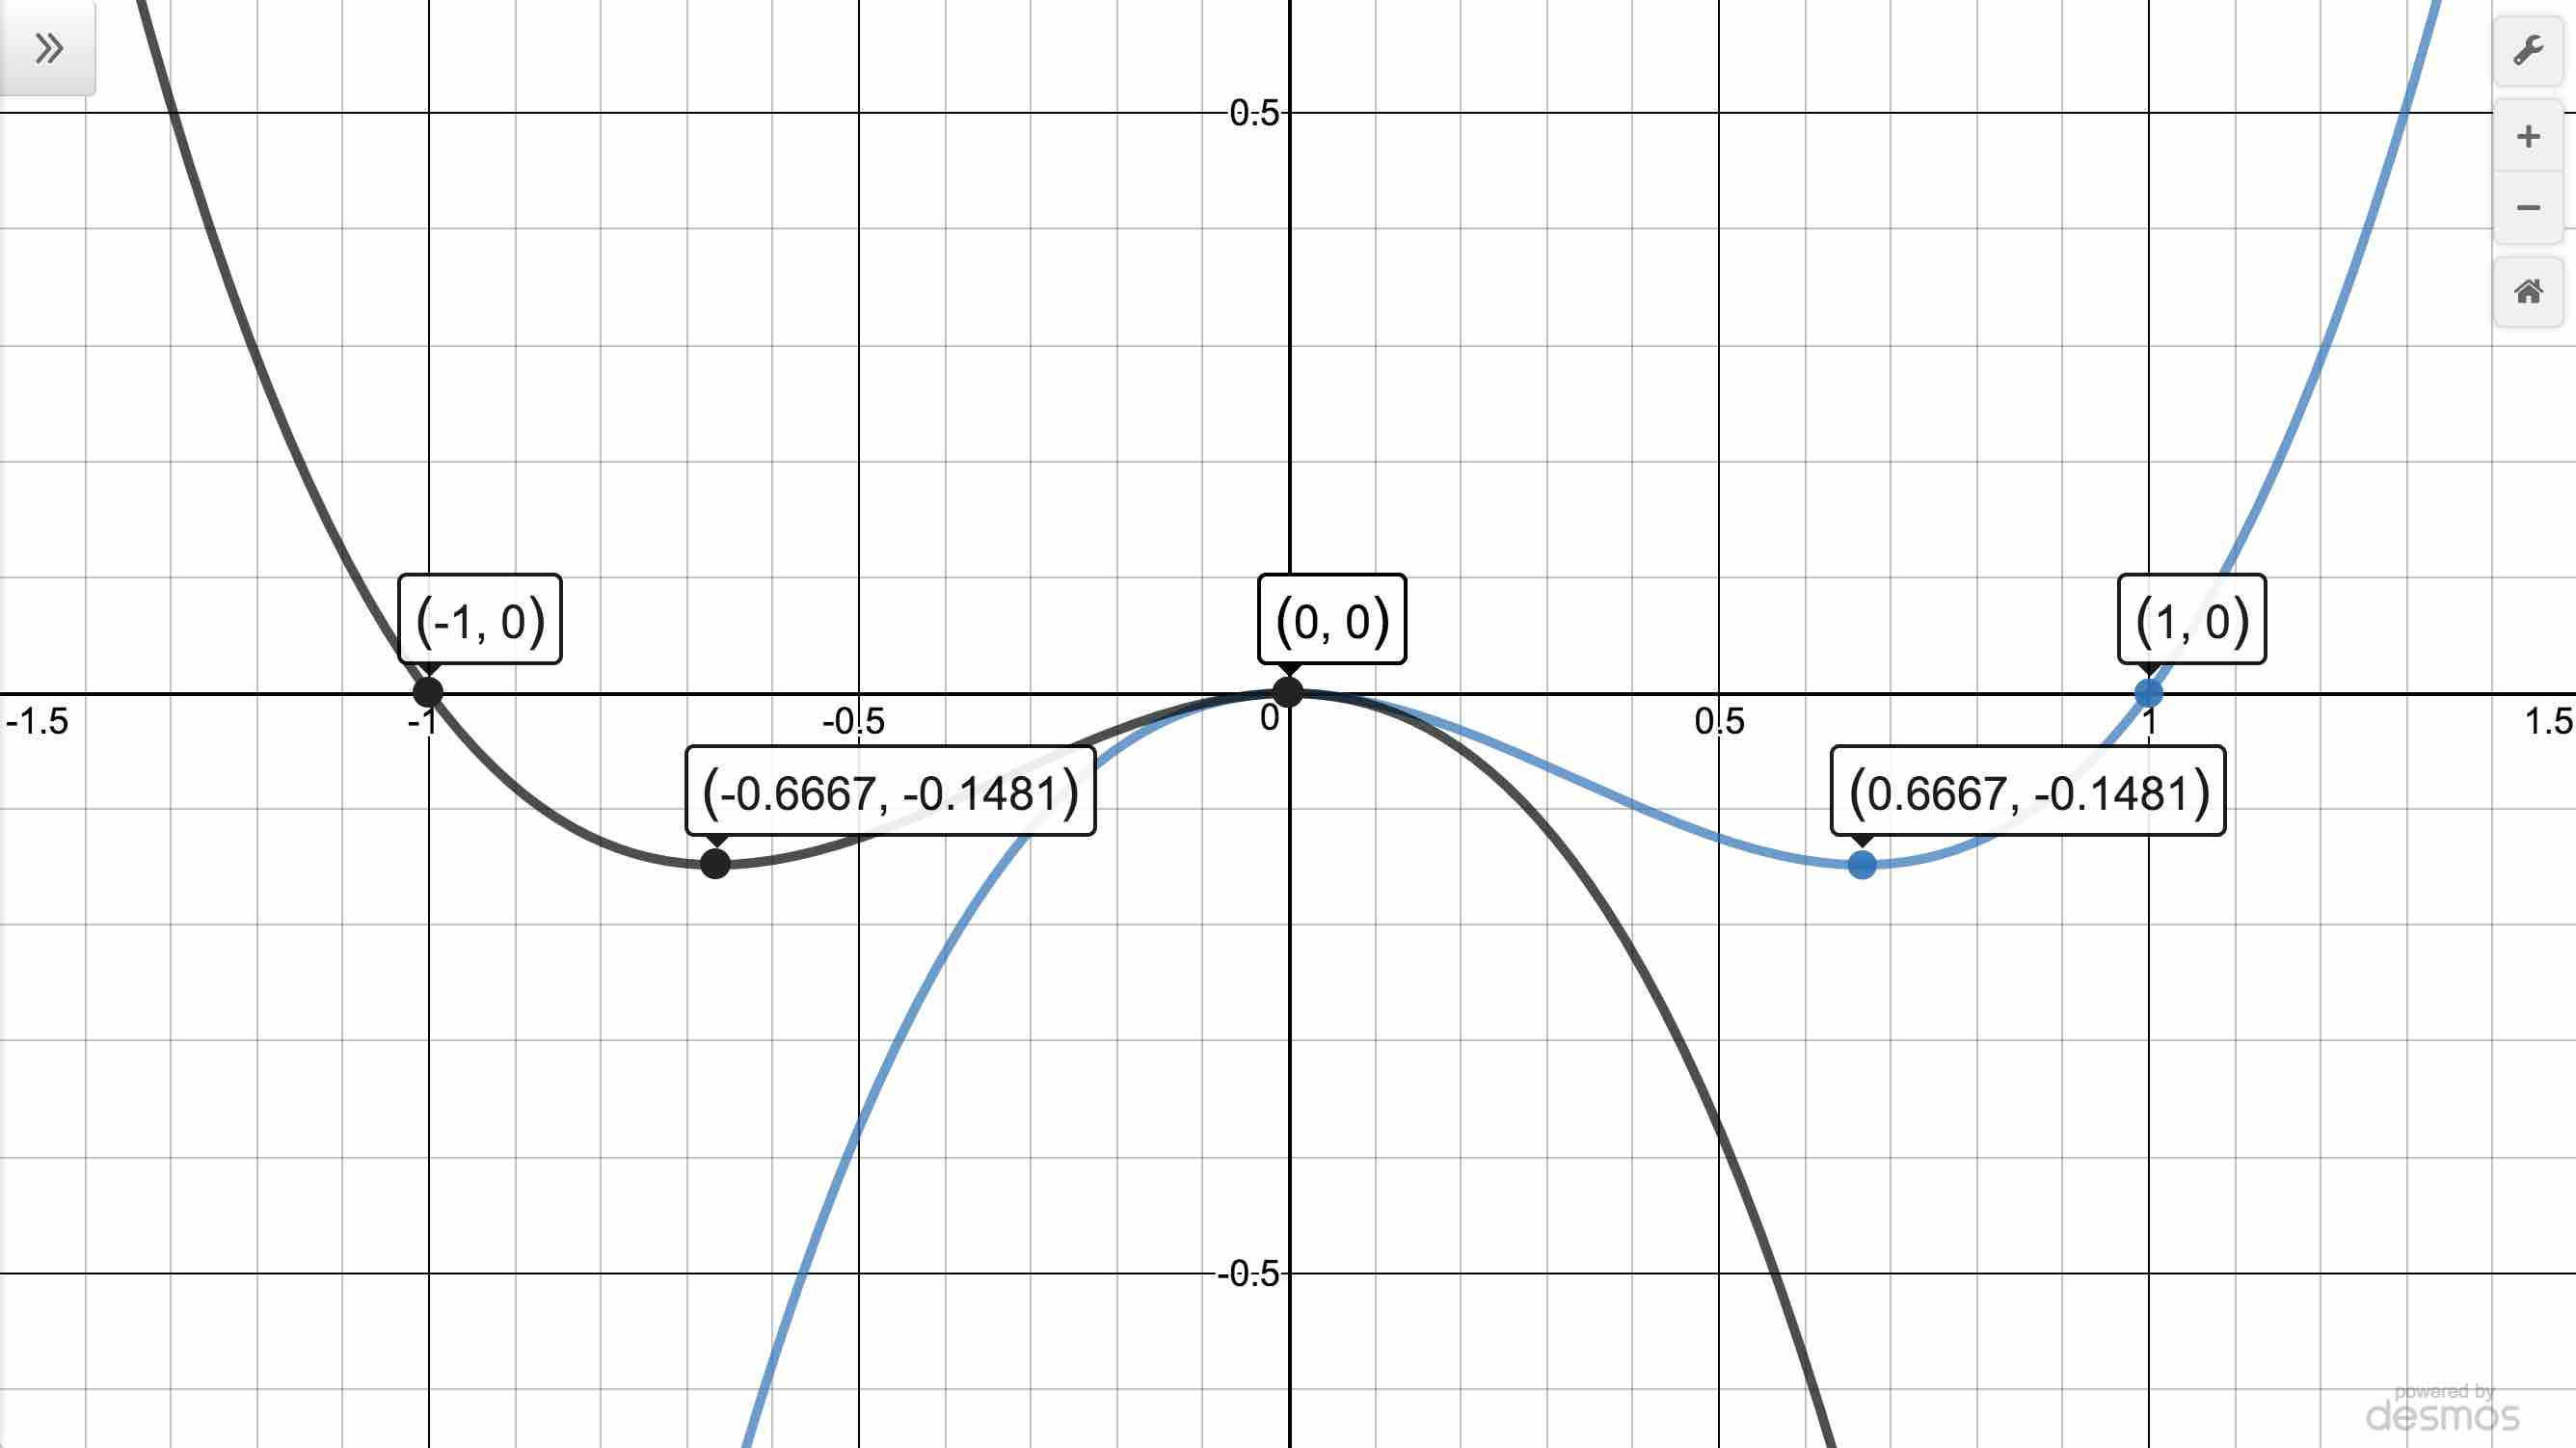
\includegraphics[width=3in]{./TransformationsGraphics/TransformationsEx02a.jpg} & 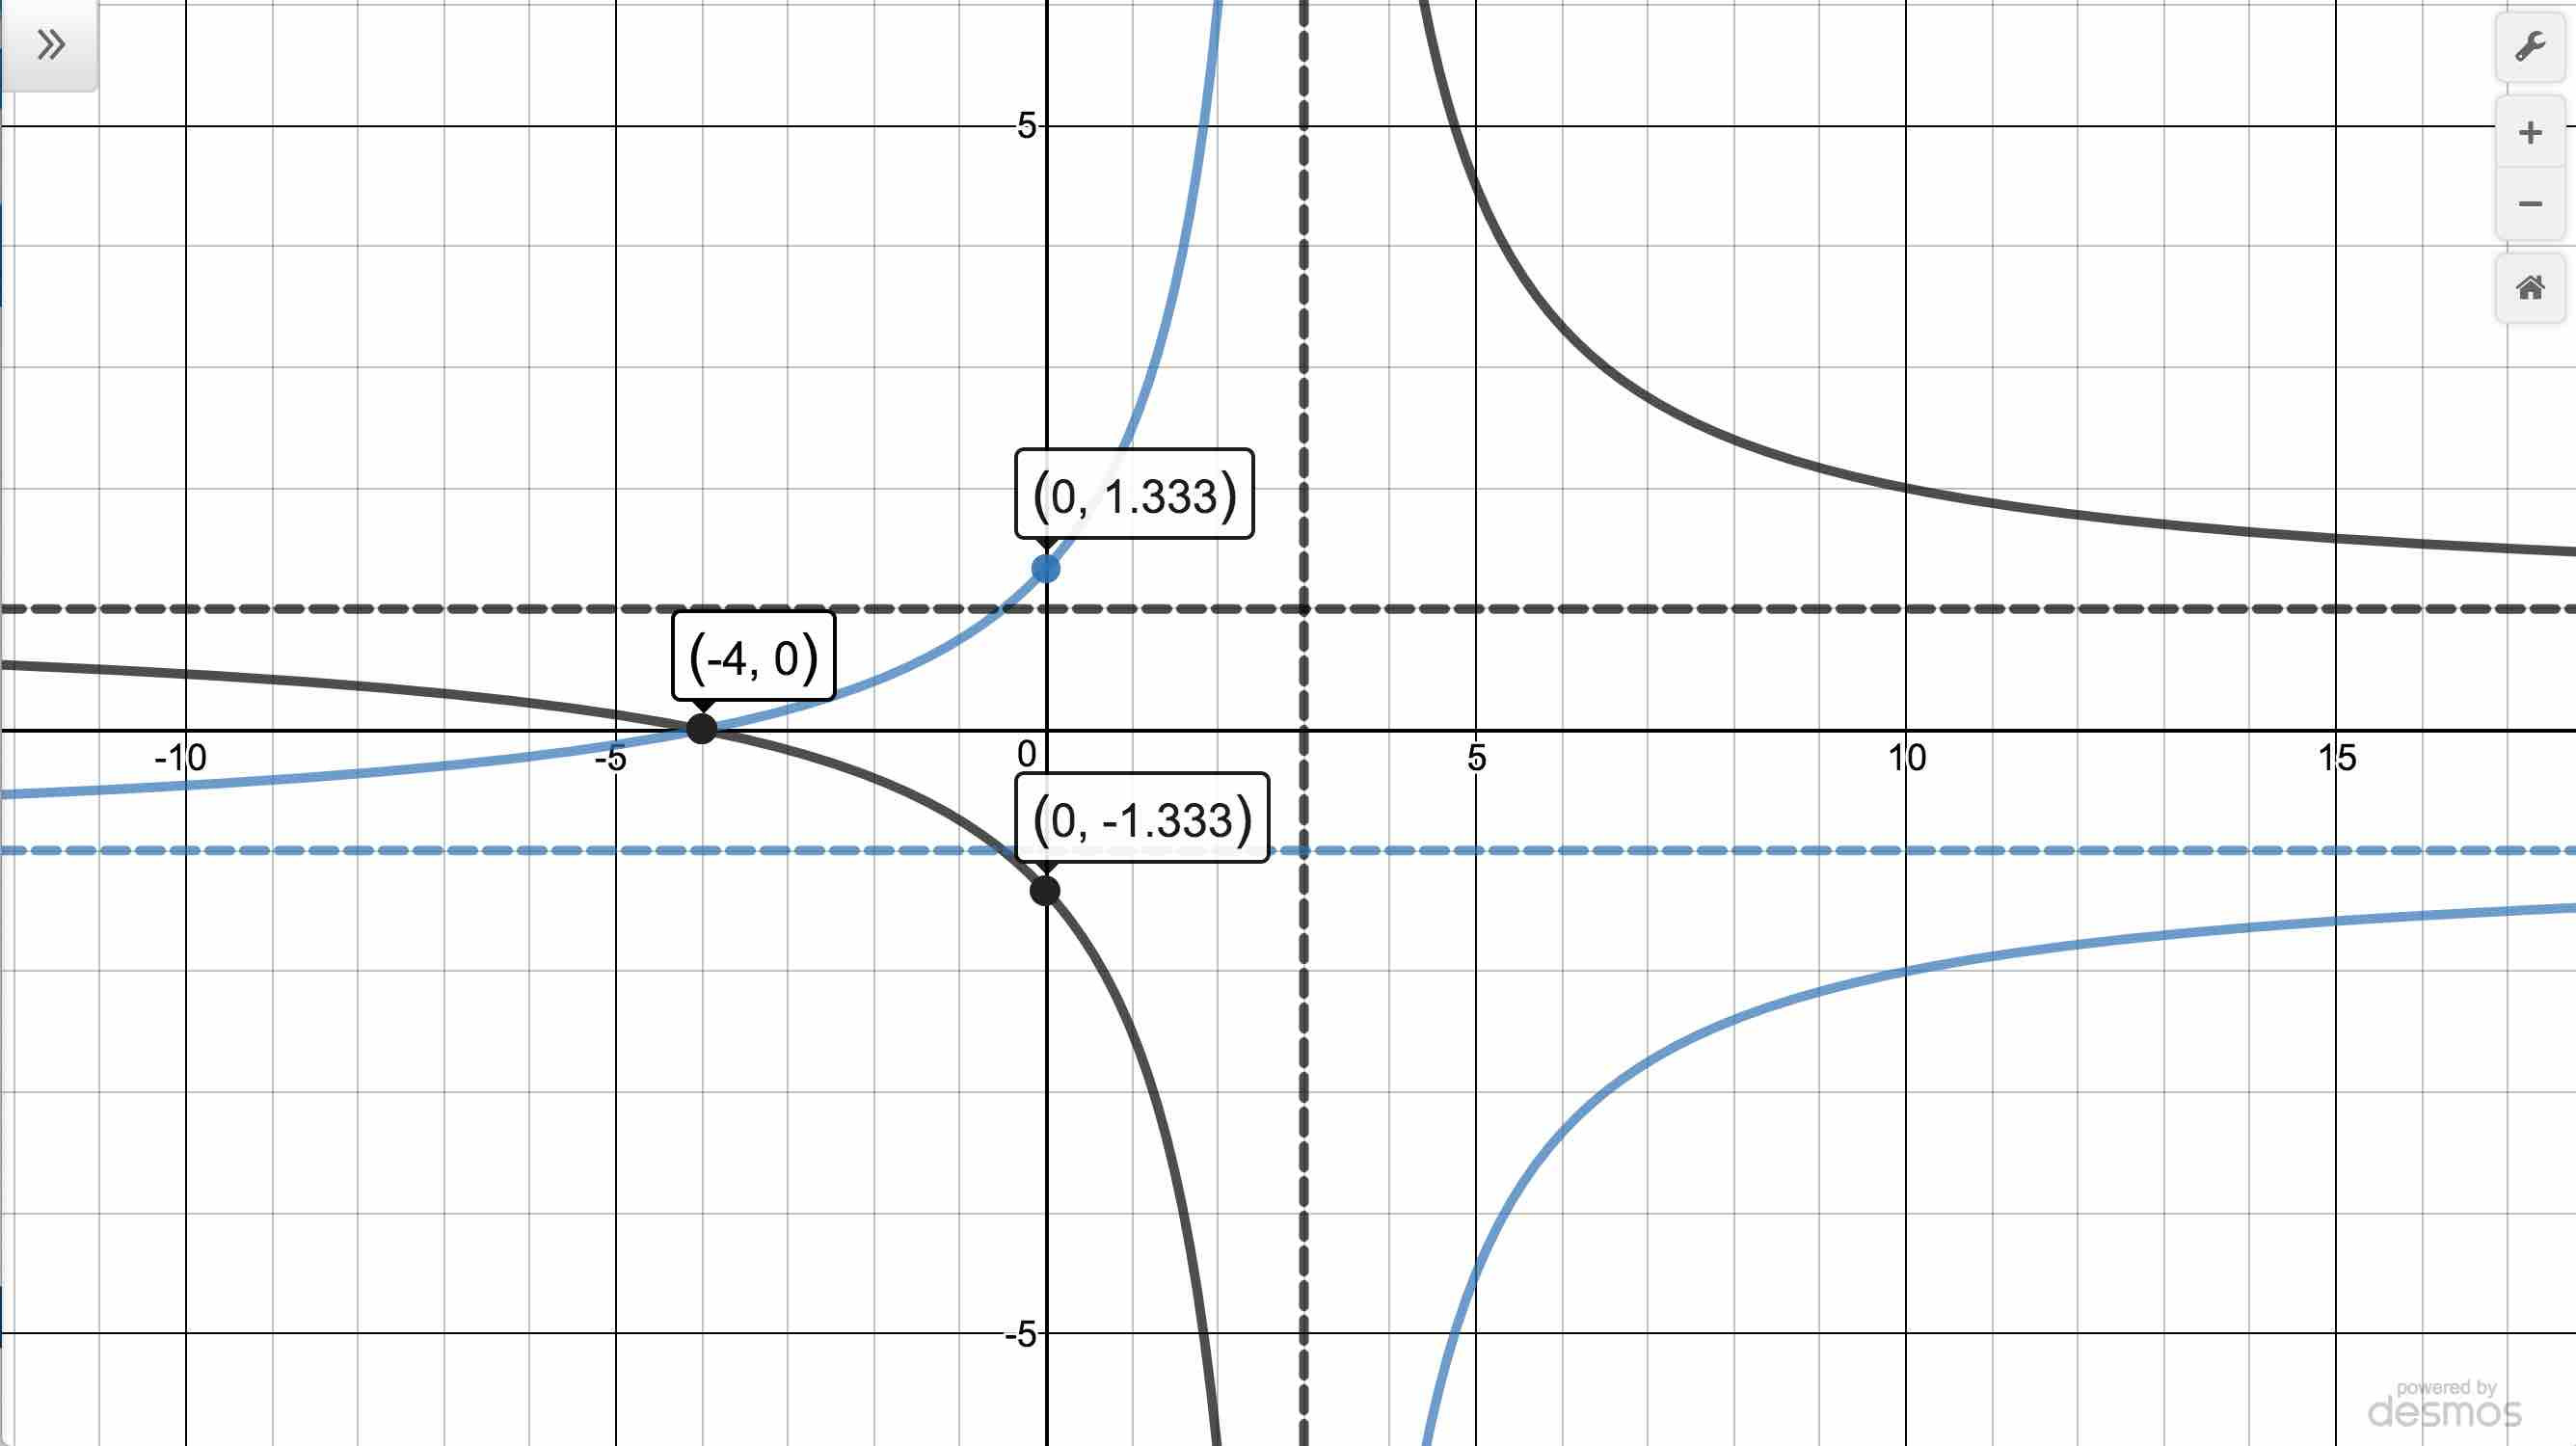
\includegraphics[width=3in]{./TransformationsGraphics/TransformationsEx02b.jpg} \\

$t =  s^3-s^2$ (lighter color)  and $t=-s^3-s^2$  &  $y = \dfrac{t+4}{3-t}$ (lighter color) and $y =  \dfrac{t+4}{t-3}$ \\

\end{tabular}

\end{center} 
 
\item
 
 \begin{enumerate}
 
 \item We have two transformations indicated with the formula $F(x) = f(-x)+1$:  a reflection across the $y$-axis and a vertical shift.  Working from the inside out, we first tackle the reflection.  Per Theorem \ref{reflections}, to obtain the graph of $y=f(-x)$ from $y=f(x)$, we multiply each of the $x$-coordinates of each of the points on the graph of $y=f(x)$ by $(-1)$.
 
 
 \[ \begin{array}{ccc}

\begin{mfpic}[15]{-3}{3}{-1}{6}
\axes
\tlabel[cc](3,-0.5){\scriptsize $x$}
\tlabel[cc](0.5,6){\scriptsize $y$}
\xmarks{-2, -1, 0, 1, 2}
\ymarks{ 0, 1, 2, 3,4,5}
\tcaption{\scriptsize $y = f(x)$}
\tlpointsep{4pt}
\scriptsize
\tlabel[cc](1, 1){$(0,1)$}
\tlabel[cc](2, 2){$(1,2)$}
\tlabel[cc](2.75, 4){$(2,4)$}
\axislabels {x}{{\scriptsize $-2 \hspace{7pt}$} -2,{\scriptsize $-1 \hspace{7pt}$} -1,{$1$} 1, {$2$} 2}
\axislabels {y}{{$2$} 2,{$3$} 3,{$4$} 4,{$5$} 5}
\normalsize
\penwd{1.25pt}
\arrow \reverse \arrow \function{-2.5, 2.5, 0.1}{2**x}
\point[4pt]{(0,1), (1,2), (2,4)}
\end{mfpic}


&

\stackrel{\stackrel{\mbox{\scriptsize reflect across $y$-axis}}{\xrightarrow{\hspace{1in}}}}{\mbox{ \scriptsize multiply each $x$-coordinate by $-1$}} 

&

\begin{mfpic}[15]{-3}{3}{-1}{6}
\axes
\tlabel[cc](3,-0.5){\scriptsize $x$}
\tlabel[cc](0.5,6){\scriptsize $y$}
\xmarks{-2, -1, 0, 1, 2}
\ymarks{ 0, 1, 2, 3,4,5}
\tcaption{\scriptsize $y = f(-x)$}
\tlpointsep{4pt}
\scriptsize
\tlabel[cc](-1, 1){$(0,1)$}
\tlabel[cc](-2.25, 2){$(-1,2)$}
\tlabel[cc](-3.25, 4){$(-2,4)$}
\axislabels {x}{{\scriptsize $-2 \hspace{7pt}$} -2,{\scriptsize $-1 \hspace{7pt}$} -1,{$1$} 1, {$2$} 2}
\axislabels {y}{{$2$} 2,{$3$} 3,{$4$} 4,{$5$} 5}
\normalsize
\penwd{1.25pt}
\arrow \reverse \arrow \function{-2.5, 2.5, 0.1}{2**(-x)}
\point[4pt]{(0,1), (-1,2), (-2,4)}
\end{mfpic}


\end{array}\]

Next, we use Theorem \ref{vshifts} to obtain the graph of $y =f(-x)+1$ from the graph of $y = f(-x)$ by adding $1$ to each of the $y$-coordinates of each of the points on the graph of $y = f(-x)$.  This shifts the graph of $y=f(-x)$ up one unit.  Note, the horizontal asymptote $y=0$ is also shifted up $1$ unit to $y=1$.

 
 \[ \begin{array}{ccc}

\begin{mfpic}[15]{-3}{3}{-1}{6}
\axes
\tlabel[cc](3,-0.5){\scriptsize $x$}
\tlabel[cc](0.5,6){\scriptsize $y$}
\xmarks{-2, -1, 0, 1, 2}
\ymarks{ 0, 1, 2, 3,4,5}
\tcaption{\scriptsize $y = f(-x)$}
\tlpointsep{4pt}
\scriptsize
\tlabel[cc](-1, 1){$(0,1)$}
\tlabel[cc](-2.25, 2){$(-1,2)$}
\tlabel[cc](-3.25, 4){$(-2,4)$}
\axislabels {x}{{\scriptsize $-2 \hspace{7pt}$} -2,{\scriptsize $-1 \hspace{7pt}$} -1,{$1$} 1, {$2$} 2}
\axislabels {y}{{$2$} 2,{$3$} 3,{$4$} 4,{$5$} 5}
\normalsize
\penwd{1.25pt}
\arrow \reverse \arrow \function{-2.5, 2.5, 0.1}{2**(-x)}
\point[4pt]{(0,1), (-1,2), (-2,4)}
\end{mfpic}


&

\stackrel{\stackrel{\mbox{\scriptsize shift up $1$ unit}}{\xrightarrow{\hspace{1in}}}}{\mbox{ \scriptsize add $1$ to each $y$-coordinate}} 

&

\begin{mfpic}[15]{-3}{3}{-1}{6}
\axes
\tlabel[cc](3,-0.5){\scriptsize $x$}
\tlabel[cc](0.5,6){\scriptsize $y$}
\xmarks{-2, -1, 0, 1, 2}
\ymarks{ 0, 1, 2, 3,4,5}
\tcaption{\scriptsize $y = f(-x)+1=F(x)$}
\tlpointsep{4pt}
\scriptsize
\tlabel[cc](-1, 2){$(0,2)$}
\tlabel[cc](-2.25, 3){$(-1,3)$}
\tlabel[cc](-3.25, 5){$(-2,5)$}
\axislabels {x}{{\scriptsize $-2 \hspace{7pt}$} -2,{\scriptsize $-1 \hspace{7pt}$} -1,{$1$} 1, {$2$} 2}
\axislabels {y}{{$3$} 3,{$4$} 4,{$5$} 5}
\normalsize
\dashed \polyline{(-3,1), (3,1)}
\penwd{1.25pt}
\arrow \reverse \arrow \function{-2.5, 2.5, 0.1}{2**(-x)+1}
\point[4pt]{(0,2), (-1,3), (-2,5)}
\end{mfpic}


\end{array}\]

To check our answer, we begin with the point $(0,2)$.  Substituting $x=0$ into $y=f(-x)+1$, we get $y=f(-0)+1 = f(0)+1$.  Since the point $(0,1)$ is on the graph of $f$, we know $f(0) = 1$.  Hence, $y = f(0)+1= 1+1=2$, so $(0,2)$ is, indeed, on the graph of $y=f(-x)+1$.  We leave it to the reader to check the remaining points.

 
  \item In order to graph $F(x)= 1 - f(2-x)$, we first rewrite as $F(x) = -f(-x+2)+1$ and note there are \textit{four} modifications to the formula $f(x)$ indicated here.  
  
  \smallskip
  
  Working from the inside out, we see we have a reflection about the $y$-axis indicated as well as a horizontal shift.  From our work above, we know we first handle the shift:  that is, we apply Theorem \ref{hshifts} to  graph $y=f(x+2) = f(x-(-2))$ by adding $-2$ to (subtracting $2$ from) the $x$-coordinates of the points on the graph of $y=f(x)$.
  
   \[ \begin{array}{ccc}

\begin{mfpic}[15]{-3}{3}{-1}{6}
\axes
\tlabel[cc](3,-0.5){\scriptsize $x$}
\tlabel[cc](0.5,6){\scriptsize $y$}
\xmarks{-2, -1, 0, 1, 2}
\ymarks{ 0, 1, 2, 3,4,5}
\tcaption{\scriptsize $y = f(x)$}
\tlpointsep{4pt}
\scriptsize
\tlabel[cc](1, 1){$(0,1)$}
\tlabel[cc](2, 2){$(1,2)$}
\tlabel[cc](2.75, 4){$(2,4)$}
\axislabels {x}{{\scriptsize $-2 \hspace{7pt}$} -2,{\scriptsize $-1 \hspace{7pt}$} -1,{$1$} 1, {$2$} 2}
\axislabels {y}{{$2$} 2,{$3$} 3,{$4$} 4,{$5$} 5}
\normalsize
\penwd{1.25pt}
\arrow \reverse \arrow \function{-2.5, 2.5, 0.1}{2**x}
\point[4pt]{(0,1), (1,2), (2,4)}
\end{mfpic}


&

\stackrel{\stackrel{\mbox{\scriptsize shift left $2$ units}}{\xrightarrow{\hspace{1in}}}}{\mbox{ \scriptsize subtract $2$ from each $x$-coordinate}} 

&

\begin{mfpic}[15]{-5}{1}{-1}{6}
\axes
\tlabel[cc](1,-0.5){\scriptsize $x$}
\tlabel[cc](0.5,6){\scriptsize $y$}
\xmarks{-4,-3, -2, -1, 0}
\ymarks{ 0, 1, 2, 3,4,5}
\tcaption{\scriptsize $y = f(x+2)$}
\tlpointsep{4pt}
\scriptsize
\tlabel[cc](-3.25, 1){$(-2,1)$}
\tlabel[cc](-2.25, 2){$(-1,2)$}
\tlabel[cc](-1, 4){$(0,4)$}
\axislabels {x}{{\scriptsize $-4 \hspace{7pt}$} -4,{\scriptsize $-3 \hspace{7pt}$} -3,{\scriptsize $-2 \hspace{7pt}$} -2,{\scriptsize $-1 \hspace{7pt}$} -1}
\axislabels {y}{{$2$} 2,{$5$} 5}
\normalsize
\penwd{1.25pt}
\arrow \reverse \arrow \function{-4.5, 0.5, 0.1}{2**(x+2)}
\point[4pt]{(-2,1), (-1,2), (0,4)}
\end{mfpic}


\end{array}\]

Next, we use Theorem \ref{reflections} to graph $y=f(-x+2)$ starting with the graph of $y = f(x+2)$ by multiplying each of the $x$-coordinates of the points of the graph of $y=f(x+2)$ by $-1$.  This reflects the graph of $f(x+2)$ about the $y$-axis.

 \[ \begin{array}{ccc}

\begin{mfpic}[15]{-5}{1}{-1}{6}
\axes
\tlabel[cc](1,-0.5){\scriptsize $x$}
\tlabel[cc](0.5,6){\scriptsize $y$}
\xmarks{-4,-3, -2, -1, 0}
\ymarks{ 0, 1, 2, 3,4,5}
\tcaption{\scriptsize $y = f(x+2)$}
\tlpointsep{4pt}
\scriptsize
\tlabel[cc](-3.25, 1){$(-2,1)$}
\tlabel[cc](-2.25, 2){$(-1,2)$}
\tlabel[cc](-1, 4){$(0,4)$}
\axislabels {x}{{\scriptsize $-4 \hspace{7pt}$} -4,{\scriptsize $-3 \hspace{7pt}$} -3,{\scriptsize $-2 \hspace{7pt}$} -2,{\scriptsize $-1 \hspace{7pt}$} -1}
\axislabels {y}{{$2$} 2,{$5$} 5}
\normalsize
\penwd{1.25pt}
\arrow \reverse \arrow \function{-4.5, 0.5, 0.1}{2**(x+2)}
\point[4pt]{(-2,1), (-1,2), (0,4)}
\end{mfpic}


&

\stackrel{\stackrel{\mbox{\scriptsize reflect about the $y$-axis}}{\xrightarrow{\hspace{1in}}}}{\mbox{ \scriptsize multiply each $x$-coordinate by $-1$}} 

&

\begin{mfpic}[15]{-1}{5}{-1}{6}
\axes
\tlabel[cc](5,-0.5){\scriptsize $x$}
\tlabel[cc](0.5,6){\scriptsize $y$}
\xmarks{0,1,2,3,4}
\ymarks{ 0, 1, 2, 3,4,5}
\tcaption{\scriptsize $y = f(-x+2)$}
\tlpointsep{4pt}
\scriptsize
\tlabel[cc](3, 1){$(2,1)$}
\tlabel[cc](1.75, 2){$(1,2)$}
\tlabel[cc](1, 4){$(0,4)$}
\axislabels {x}{{$1$} 1, {$2$} 2,{$3$} 3, {$4$} 4}
\axislabels {y}{{$2$} 2,{$3$} 3,{$4$} 4}
\normalsize
\penwd{1.25pt}
\arrow \reverse \arrow \function{-0.5, 4.5, 0.1}{2**(-x+2)}
\point[4pt]{(2,1), (1,2), (0,4)}
\end{mfpic}


\end{array}\]

We have the graph of $y=f(-x+2)$ and need to build towards the graph of $y=-f(-x+2)+1$.  The transformations that remain are a reflection about the $x$-axis and a vertical shift.  The question is which to do first.  

\smallskip

Once again, we can think algebraically about the problem.  We know the point $(0,1)$ is on the graph of $f$ which means $f(0) = 1$.  This point corresponds to the point $(2,1)$ on the graph of $f(-x+2)$.  Indeed, when we substitute $x=2$ into $y=f(-x+2)$, we get $y = f(-2+2) = f(0) =1$.  

\smallskip

If we substitute $x=2$ into the formula $y=-f(-x+2)+1$, we get $y=-f(-2+2)+1 = -f(0)+1  = -1(1)+1 = 0$.  That is, we first multiply the $y$-coordinate of $(2,1)$ by $-1$ then add $1$.  This suggests we take care of the reflection about the $x$-axis first, then the vertical shift.  

\smallskip

We proceed below to obtain the graph of $y=-f(-x+2)$ from $y=f(-x+2)$ by multiplying each of the $y$-coordinates on the graph of $y=f(-x+2)$ by $-1$.  Note the horizontal asymptote remains unchanged: $y=(-1)(0) = 0$.

 \[ \begin{array}{ccc}

\begin{mfpic}[15]{-1}{5}{-1}{6}
\axes
\tlabel[cc](5,-0.5){\scriptsize $x$}
\tlabel[cc](0.5,6){\scriptsize $y$}
\xmarks{0,1,2,3,4}
\ymarks{ 0, 1, 2, 3,4,5}
\tcaption{\scriptsize $y = f(-x+2)$}
\tlpointsep{4pt}
\scriptsize
\tlabel[cc](3, 1){$(2,1)$}
\tlabel[cc](1.75, 2){$(1,2)$}
\tlabel[cc](1, 4){$(0,4)$}
\axislabels {x}{{$1$} 1, {$2$} 2,{$3$} 3, {$4$} 4}
\axislabels {y}{{$2$} 2,{$3$} 3,{$4$} 4}
\normalsize
\penwd{1.25pt}
\arrow \reverse \arrow \function{-0.5, 4.5, 0.1}{2**(-x+2)}
\point[4pt]{(2,1), (1,2), (0,4)}
\end{mfpic}

&

\stackrel{\stackrel{\mbox{\scriptsize reflect about the $x$-axis}}{\xrightarrow{\hspace{1in}}}}{\mbox{ \scriptsize multiply each $y$-coordinate by $-1$}} 

&

\begin{mfpic}[15]{-1}{5}{-6}{1}
\axes
\tlabel[cc](5,-0.5){\scriptsize $x$}
\tlabel[cc](0.5,1){\scriptsize $y$}
\xmarks{0,1,2,3,4}
\ymarks{ 0, -1, -2, -3,-4,- 5}
\tcaption{\scriptsize $y = - f(-x+2)$}
\tlpointsep{4pt}
\scriptsize
\tlabel[cc](3, -1.25){$(2,-1)$}
\tlabel[cc](2, -2.25){$(1,-2)$}
\tlabel[cc](1, -4){$(0,-4)$}
\axislabels {x}{{$1$} 1, {$2$} 2}
\axislabels {y}{{$-2$} -2,{$-3$} -3,{$-4$} -4}
\normalsize
\penwd{1.25pt}
\arrow \reverse \arrow \function{-0.5, 4.5, 0.1}{0-2**(-x+2)}
\point[4pt]{(2,-1), (1,-2), (0,-4)}
\end{mfpic}

\end{array}\]

Finally, we take care of the vertical shift.  Per Theorem \ref{vshifts}, we graph $y=-f(-x+2)+1$ by adding $1$ to the $y$-coordinates of each of the points on the graph of $y=-f(-x+2)$.  This moves the graph up one unit, including the horizontal asymptote:  $y=0+1 = 1$.

 \[ \begin{array}{ccc}

\begin{mfpic}[15]{-1}{5}{-6}{1}
\axes
\tlabel[cc](5,-0.5){\scriptsize $x$}
\tlabel[cc](0.5,1){\scriptsize $y$}
\xmarks{0,1,2,3,4}
\ymarks{ 0, -1, -2, -3,-4,- 5}
\tcaption{\scriptsize $y = - f(-x+2)$}
\tlpointsep{4pt}
\scriptsize
\tlabel[cc](3, -1.25){$(2,-1)$}
\tlabel[cc](2, -2.25){$(1,-2)$}
\tlabel[cc](1, -4){$(0,-4)$}
\axislabels {x}{{$1$} 1, {$2$} 2}
\axislabels {y}{{$-2$} -2,{$-3$} -3,{$-4$} -4}
\normalsize
\penwd{1.25pt}
\arrow \reverse \arrow \function{-0.5, 4.5, 0.1}{0-2**(-x+2)}
\point[4pt]{(2,-1), (1,-2), (0,-4)}
\end{mfpic}

&

\stackrel{\stackrel{\mbox{\scriptsize shift up $1$ unit}}{\xrightarrow{\hspace{1in}}}}{\mbox{ \scriptsize add $1$ to each of the $y$-coordinates}} 

&

\begin{mfpic}[15]{-1}{5}{-5}{2}
\axes
\tlabel[cc](5,-0.5){\scriptsize $x$}
\tlabel[cc](0.5,2){\scriptsize $y$}
\xmarks{0,1,2,3,4}
\ymarks{ 1, 0, -1, -2, -3,-4}
\tcaption{\scriptsize $y = - f(-x+2)+1 = F(x)$}
\tlpointsep{4pt}
\scriptsize
\tlabel[cc](2.5, -0.5){$(2,0)$}
\tlabel[cc](2, -1.25){$(1,-1)$}
\tlabel[cc](1, -3){$(0,-3)$}
\axislabels {x}{{$1$} 1}
\axislabels {y}{{$-2$} -2,{$-3$} -3,{$1$} 1}
\normalsize
\dashed \polyline{(-1,1), (5,1)}
\penwd{1.25pt}
\arrow \reverse \arrow \function{-0.5, 4.5, 0.1}{1-2**(-x+2)}
\point[4pt]{(2,0), (1,-1), (0,-3)}
\end{mfpic}

\end{array}\]

To check, we begin with the point $(2,0)$.  Substituting $x=2$ into $y=1 - f(2-x)$, we obtain $y = 1-f(2-2) = 1-f(0)$.  Since $(0,1)$ is on the graph of $f$, we know $f(0) = 1$.  This means $y = 1-f(2-2) = 1-f(0)= 1-1 = 0$.  This proves $(2,0)$ is on the graph of  $y=1 - f(2-x)$, and we recommend the reader check the remaining points.
 
 \end{enumerate}

 \item With the transformations at our disposal,  our task amounts to finding values of $h$ and $k$ and choosing between signs $\pm$  so that  $g(x) = \pm f( \pm x - h) + k$.  
 
 \smallskip
 
 Based on the horizontal asymptote, $y=4$, we choose $k=4$.  Note, however, in the graph of $y=f(x)+4$, the entire graph is \textit{above} the line $y=4$.  Since the graph of $g$ approaches the asymptote from below, we know  $y=-f(\pm x-h)+4$.  
 
 \smallskip
 
 Hence, two of transformations applied to the graph of $f$ are a reflection across the $x$-axis followed by a shift up $4$ units.  This means the point $(0,1)$ on the graph of $f$ must correspond to the point $(-1,3)$ on the graph of $g$, since these are the points closest to the asymptote on each graph.  
  
  \smallskip
  
Likewise, the points $(1,2)$ and $(2,4)$ on the graph of $f$ must correspond to $(0,2)$ and $(1,0)$, respectively, on the graph of $g$.  Looking at the $x$-coordinates only, we have $x=0$ moves to $x=-1$, $x=1$ moves to $x=0$, and $x=2$ moves to $x=1$.  Hence, the net effect on the $x$-values is a shift left $1$ unit.  Hence, we guess the formula for $g(x)$ to be $g(x) = -f(x+1)+4$.  

\smallskip

We can readily check by going through the transformations:  first, shift left $1$ unit; next,  reflect across the $x$-axis;  finally, shift up $4$.  We leave it to the reader to verify that tracking each of the points on the graph of $f$ along with the horizontal asymptote through this sequence of transformations results in the graph of $g$.  
 
 
 \smallskip
 
 
 One way to recover the graph of $f$ from the graph of $g$ is to reverse the process by which we obtained $g$ from $f$.  The challenge here comes from the fact that two different operations were done which affected the $y$-values:  reflection and shifting - and the order in which these are done matters.  
 
 \smallskip
 
 To motivate our methodology, let's consider a more down-to-earth example like putting on socks and then putting on shoes.  Unless we're very talented,  to reverse this process, we take off the shoes first, then the socks - that is, we undo each step in the reverse order.\footnote{We'll have more to say about this sort of thing in Section \ref{InverseFunctions}.}  In the same way, when we think about reversing the steps transforming the graph of $f$ to the graph of $g$, we need to undo each transformation in the opposite order.  
 
 \smallskip
 
 To review, we obtained the graph of $g$ from the graph of $f$ by first shifting the graph to the left $1$ unit, then reflecting the graph about the $x$-axis, then, finally, shifting the graph up $4$ units.  Hence, we first undo the vertical shift.  Instead of shifting the graph \textit{up} four units, we shift the graph \textit{down} four units.  This takes the graph of $y = g(x)$ to $y = g(x)-4$.  
 
 \smallskip
 
 Next, we have to undo the refection across the $x$-axis.  Thinking at the level of points, to recover the point $(a,b)$ from its reflection across the $x$-axis, $(a,-b)$, we simply reflect across the $x$-axis again: $(a,-(-b)) = (a,b)$.  Per Theorem \ref{reflections}, this takes the graph the graph of $y = g(x)-4$ to the graph of $y = -[g(x)-4] = -g(x) + 4$.\footnote{To see this better, let us temporarily write $F(x) = g(x)-4$.  Theorem \ref{reflections} tells us to reflect the graph of $F$ about the $x$-axis, graph $y=-F(x) = - [g(x)-4] = -g(x)+4$.} 
 
 \smallskip
 
 Last, to undo moving the graph to the \textit{left} $1$ unit, we move the graph of $y=-g(x)+4$ to the \textit{right} $1$ unit.  Per Theorem \ref{hshifts}, we accomplish this by graphing $y = -g(x-1)+4$.  We leave it to the reader to start with the graph of $y=g(x)$ and graph $y = -g(x-1)+4$ and show it matches the graph of $y=f(x)$. \qed
    
 \end{enumerate}

\end{ex}

Some remarks about Example \ref{reflectionsex}  are in order. In number \ref{twotransxrefex} above, to find a point on the graph of $y=f(-x+8)$, we took the given $x$-coordinate on our starting graph, $2$, and subtracted $8$ first then multiplied by $-1$.  If this seems somehow `backwards' it should.  

\smallskip

When \textit{evaluating} the expression $-x+8$, the order of operations mandates we multiply by $-1$ first then add $8$.  Here, however, we weren't \textit{evaluating} an expression - we were \textit{solving} an equation:  $-x+8 = 2$, which meant we did the exact opposite steps in the opposite order.\footnote{Note that dividing by $-1$ is the same as multiplying by $-1$, so to keep with the `opposite steps in opposite order' theme, we could more precisely say we subtracted $8$ and \textit{divided} by $-1$.}  This exemplifies a larger theme with transformations:  when adjusting inputs, the resulting points on the graph are obtained by applying the opposite operations indicated by the formula in the opposite order of operations.



\smallskip


On the other hand, when it came to multiple transformations involving the $y$-coordinates, we followed the order of operations. As in \ref{twotransyrefex} above, when it came to applying a reflection about the $x$-axis and a vertical shift, we applied the reflection first, then the shift.  This is because instead of \textit{solving} an \textit{equation} to find the new $y$-coordinates, we were \textit{simplifying }an \textit{expression}.  Again, this is an example of a much larger theme:  when adjusting outputs, the resulting points on the graph are obtained by applying the stated operations in the usual order.


\smallskip


Last but not least, in number \ref{gfromfrefex}, to find $f$ in terms of $g$, we reversed the steps used to transform $f$ into $g$.  Another tact is to approach the problem in the same way we approached transforming $f$ into $g$: namely, starting with the graph of $g$, determine values $h$ and $k$ and signs $\pm$ so that $f(x) = \pm g(\pm x - h) + k$.  We leave this to the reader.


\subsection{Scalings}
\label{Scaling}

We now turn our attention to our last class of transformations: \textbf{scalings}.  A thorough discussion of scalings can get complicated because they are not as straight-forward as the previous transformations.  A quick review of what we've covered so far, namely vertical shifts, horizontal shifts and reflections, will show you why those transformations are known as \index{transformation ! rigid}\textbf{rigid transformations}.  

\smallskip

Simply put, rigid transformations preserve the distances between points on the graph -  only their position and orientation in the plane change.\footnote{Another word that can be used here instead of `rigid transformation' is `isometry' - meaning `same distance.'}  If, however, we wanted to make a new graph twice as tall as a given graph, or one-third as wide, we would be affecting the distance between points. These sorts of transformations are hence called \textbf{non-rigid}\index{transformation ! non-rigid}.  As always, we motivate the general theory with an example.

\smallskip

Suppose we wish to graph the function $g(x) =2 f(x)$ where $f(x)$ is the function whose graph is given at the beginning of the section. From its graph, we can build a table of values for $g$ as before.

\begin{center}

\begin{tabular}{m{2in}m{3in}}

\begin{mfpic}[15]{-1}{6}{-1}{6}
\tlabel[cc](-1,1){\scriptsize $(0,1)$}
\tlabel[cc](2,3.5){\scriptsize $(2,3)$}
\tlabel[cc](4,2.5){\scriptsize $(4,3)$}
\tlabel[cc](5,5.5){\scriptsize $(5,5)$}
\tlabel[cc](6,-0.5){\scriptsize $x$}
\tlabel[cc](0.5,6){\scriptsize $y$}
\tcaption{\scriptsize $y=f(x)$}
\axes
\xmarks{1,2,3,4,5}
\ymarks{1,2,3,4,5}
\tlpointsep{4pt}
\axislabels {x}{{\scriptsize $1$} 1, {\scriptsize $2$} 2, {\scriptsize $3$} 3, {\scriptsize $4$} 4, {\scriptsize $5$} 5}
\axislabels {y}{{\scriptsize $2$} 2, {\scriptsize $3$} 3, {\scriptsize $4$} 4, {\scriptsize $5$} 5}
\penwd{1.25pt}
\polyline{(0,1), (2,3), (4,3), (5,5)}
\point[4pt]{(0,1), (2,3), (4,3), (5,5)}
\end{mfpic}
 
&

\[ \begin{array}{|c||c|c|c|c|}  

\hline

 x & (x,f(x)) & f(x) & g(x)=2f(x) & (x, g(x)) \\ \hline
0  & (0,1)& 1 & 2 &(0, 2) \\  \hline
2 & (2,3) & 3 &  6 &(2,6) \\  \hline
4 & (4,3) & 3 &  6 &(4, 6) \\  \hline
5 & (5,5) & 5 &  10 &( 5 ,10) \\  \hline

\end{array} \] 

\end{tabular}

\end{center}

Graphing, we get:

\[ \begin{array}{ccc}

\begin{mfpic}[15]{-1}{6}{-1}{11}
\tlabel[cc](-1,1){\scriptsize $(0,1)$}
\tlabel[cc](2,3.5){\scriptsize $(2,3)$}
\tlabel[cc](4,2.5){\scriptsize $(4,3)$}
\tlabel[cc](5,5.5){\scriptsize $(5,5)$}
\tlabel[cc](6,-0.5){\scriptsize $x$}
\tlabel[cc](0.5,11){\scriptsize $y$}
\tcaption{\scriptsize $y=f(x)$}
\axes
\xmarks{1,2,3,4,5}
\ymarks{1,2,3,4,5,6,7,8,9,10}
\tlpointsep{4pt}
\axislabels {x}{{\scriptsize $1$} 1, {\scriptsize $2$} 2, {\scriptsize $3$} 3, {\scriptsize $4$} 4, {\scriptsize $5$} 5}
\axislabels {y}{{\scriptsize $2$} 2, {\scriptsize $3$} 3, {\scriptsize $4$} 4, {\scriptsize $5$} 5, {\scriptsize $6$} 6, {\scriptsize $7$} 7, {\scriptsize $8$} 8, {\scriptsize $9$} 9,  {\scriptsize $10$} 10 }
\penwd{1.25pt}
\polyline{(0,1), (2,3), (4,3), (5,5)}
\point[4pt]{(0,1), (2,3), (4,3), (5,5)}
\end{mfpic}

&

\stackrel{\stackrel{\mbox{\scriptsize vertical scaling by a factor of $2$ }}{\xrightarrow{\hspace{1.7in}}}}{\mbox{ \scriptsize multiply each $y$-coordinate by $2$}} 

&


\begin{mfpic}[15]{-1}{6}{-1}{11}
\tlabel[cc](-1,2){\scriptsize $(0,2)$}
\tlabel[cc](2,6.5){\scriptsize $(2,6)$}
\tlabel[cc](4,5.5){\scriptsize $(4,6)$}
\tlabel[cc](5,10.5){\scriptsize $(5,10)$}
\tlabel[cc](6,-0.5){\scriptsize $x$}
\tlabel[cc](0.5,11){\scriptsize $y$}
\tcaption{\scriptsize $y= 2f(x)$}
\axes
\xmarks{1,2,3,4,5}
\ymarks{1,2,3,4,5,6,7,8,9,10}
\tlpointsep{4pt}
\axislabels {x}{{\scriptsize $1$} 1, {\scriptsize $2$} 2, {\scriptsize $3$} 3, {\scriptsize $4$} 4, {\scriptsize $5$} 5}
\axislabels {y}{{\scriptsize $1$} 1, {\scriptsize $3$} 3, {\scriptsize $4$} 4, {\scriptsize $5$} 5, {\scriptsize $6$} 6, {\scriptsize $7$} 7, {\scriptsize $8$} 8, {\scriptsize $9$} 9,  {\scriptsize $10$} 10 }
\penwd{1.25pt}
\polyline{(0,2), (2,6), (4,6), (5,10)}
\point[4pt]{(0,2), (2,6), (4,6), (5,10)}
\end{mfpic}

\end{array} \]

In general, if $(a,b)$ is on the graph of $f$, then $f(a) = b$ so that $g(a) = 2 f(a) = 2b$ puts $(a,2b)$ on the graph of $g$.  In other words, to obtain the graph of $g$, we multiply all of the $y$-coordinates of the points on the graph of $f$ by $2$.  Multiplying all of the $y$-coordinates of all of the points on the graph of $f$ by $2$ causes what is known as a `vertical scaling\footnote{Also called a `vertical stretch,' `vertical expansion' or `vertical dilation' by a factor of $2$.} by a factor of $2$.'

\smallskip

If we wish to graph $y = \frac{1}{2} f(x)$, we multiply the all of the $y$-coordinates of the points on the graph of $f$ by $\frac{1}{2}$.  This creates a `vertical scaling\footnote{Also called `vertical shrink,' `vertical compression' or `vertical contraction' by a factor of $2$.} by a factor of $\frac{1}{2}$' as seen below.

\[ \begin{array}{ccc}

\begin{mfpic}[15]{-1}{6}{-1}{6}
\tlabel[cc](-1,1){\scriptsize $(0,1)$}
\tlabel[cc](2,3.5){\scriptsize $(2,3)$}
\tlabel[cc](4,2.5){\scriptsize $(4,3)$}
\tlabel[cc](5,5.5){\scriptsize $(5,5)$}
\tlabel[cc](6,-0.5){\scriptsize $x$}
\tlabel[cc](0.5,6){\scriptsize $y$}
\tcaption{\scriptsize $y=f(x)$}
\axes
\xmarks{1,2,3,4,5}
\ymarks{1,2,3,4,5}
\tlpointsep{4pt}
\axislabels {x}{{\scriptsize $1$} 1, {\scriptsize $2$} 2, {\scriptsize $3$} 3, {\scriptsize $4$} 4, {\scriptsize $5$} 5}
\axislabels {y}{{\scriptsize $2$} 2, {\scriptsize $3$} 3, {\scriptsize $4$} 4, {\scriptsize $5$} 5}
\penwd{1.25pt}
\polyline{(0,1), (2,3), (4,3), (5,5)}
\point[4pt]{(0,1), (2,3), (4,3), (5,5)}
\end{mfpic}

&

\stackrel{\stackrel{\mbox{\scriptsize vertical scaling by a factor of $\frac{1}{2}$ }}{\xrightarrow{\hspace{1.7in}}}}{\mbox{ \scriptsize multiply each $y$-coordinate by $\frac{1}{2}$}} 

&

\begin{mfpic}[15]{-1}{6}{-1}{6}
\tlabel[cc](-1,0.5){\scriptsize $\left(0,\frac{1}{2}\right)$}
\tlabel[cc](2,2){\scriptsize $\left(2,\frac{3}{2}\right)$}
\tlabel[cc](4,1){\scriptsize $\left(4,\frac{3}{2}\right)$}
\tlabel[cc](5,3){\scriptsize $\left(5,\frac{5}{2}\right)$}
\tlabel[cc](6,-0.5){\scriptsize $x$}
\tlabel[cc](0.5,6){\scriptsize $y$}
\tcaption{\scriptsize $y=\frac{1}{2} f(x)$}
\axes
\xmarks{1,2,3,4,5}
\ymarks{1,2,3,4,5}
\tlpointsep{4pt}
\axislabels {x}{{\scriptsize $1$} 1, {\scriptsize $2$} 2, {\scriptsize $3$} 3, {\scriptsize $4$} 4, {\scriptsize $5$} 5}
\axislabels {y}{{\scriptsize $1$} 1,{\scriptsize $2$} 2, {\scriptsize $3$} 3, {\scriptsize $4$} 4, {\scriptsize $5$} 5}
\penwd{1.25pt}
\polyline{(0,0.5), (2,1.5), (4,1.5), (5,2.5)}
\point[4pt]{(0,0.5), (2,1.5), (4,1.5), (5,2.5)}
\end{mfpic}

\end{array} \]

These results are generalized in the following theorem.

\smallskip

\colorbox{ResultColor}{\bbm

%\smallskip

\begin{thm} \label{vscalings}\index{graph ! vertical scaling}\textbf{Vertical Scalings.} Suppose $f$ is a function and $a>0$ is a real number. 

To graph $F(x) = af(x)$, multiply each of the $y$-coordinates of the points on the graph of $y=f(x)$ by $a$. 

\begin{itemize}

\item If $a > 1$, we say the graph of $f$ has undergone a vertical stretch\footnote{expansion, dilation} by a factor of $a$. 

\item If $0 < a < 1$, we say the graph of $f$ has undergone a vertical shrink\footnote{ compression, contraction} by a factor of $\frac{1}{a}$.

\end{itemize}

\end{thm}

\ebm}

\smallskip

The proof of Theorem \ref{vscalings} mimics the proofs of Theorems \ref{vshifts} and \ref{reflections}.  If $c$ is in the domain of $f$, then $(c, f(c))$ is on the graph of $f$ and the corresponding point on the graph of $F(x)=af(x)$ is $(c, F(c)) = (c, a f(c))$.  Comparing the points $(c, f(c))$ and $(c, a f(c))$ proves the theorem.  

\smallskip

A few remarks about Theorem \ref{vscalings} are in order.  First, a note about the verbiage.  To the authors, the words `stretch', `expansion', and `dilation' all indicate something getting bigger.  Hence, `stretched by a factor of $2$' makes sense if we are scaling something by multiplying it by $2$. Similarly, we believe words like `shrink', `compression' and `contraction' all indicate something getting smaller, so if we scale something by a factor of $\frac{1}{2}$, we would say it `shrinks by a factor of $2$' - not `shrinks by a factor of $\frac{1}{2}$'.  This is why we have written the descriptions `stretch by a factor of $a$' and `shrink by a factor of $\frac{1}{a}$' in the statement of the theorem.  

\smallskip

Second, in terms of inputs and outputs, Theorem \ref{vscalings} says multiplying the \textit{outputs} from a function by positive number $a$ causes the graph to be vertically scaled by a factor of $a$.  It is natural to ask what would happen if we multiply the \textit{inputs} of a function by a positive number.  This leads us to our last transformation of the section.

\smallskip

Referring to the graph of $f$ given at the beginning of this section, suppose we want to graph $g(x) = f(2x)$.  In other words, we are looking to see what effect multiplying the inputs to $f$ by $2$ has on its graph.  If we attempt to build a table directly, we quickly run into the same problem we had in our discussion leading up to Theorem \ref{hshifts}, as seen in the table on the left below.  

\smallskip

We solve this problem in the same way we solved this problem before.  For example, if we want to determine the point on $g$ which corresponds to the point $(2,3)$ on the graph of $f$,  we set $2x =2 $ so that $x=1$.  Substituting $x=1$ into $g(x)$, we obtain $g(1) = f(2 \cdot 1) = f(2) = 3$, so that $(1,3)$ is on the graph of $g$. Continuing in this fashion, we obtain the table on the lower right.   

\smallskip

\begin{tabular}{cc}

$ \begin{array}{|c||c|c|c|c|}  

\hline

x & (x,f(x)) & f(x)& g(x)=f(2x) & (x, g(x)) \\ \hline
0  & (0,1)& 1 & f(2 \cdot 0) = f(0) = 1   &(0, 1) \\  \hline
2 & (2,3) & 3 & f(2\cdot2) = f(4) = 3  &(2,3) \\  \hline
4 & (4,3) & 3 &  f(2 \cdot 4) = f(8) = ? &  \\  \hline
5 & (5,5) & 5 & f(2 \cdot 5) = f(10) = ?  &  \\  \hline

\end{array} $ 

&

$ \begin{array}{|r||c|c|c|}  

\hline

x & 2x & g(x)=f(2x) & (x, g(x)) \\ \hline
0 & 0 & g(0)= f(2 \cdot 0) = f(0) = 1   &(0, 0) \\  \hline
1 &  2 &  g(1)=f(2 \cdot 1) = f(2)  = 3  &(1,3) \\  \hline
2 & 4  & g(2)=f(2 \cdot 2) = f(4) = 3 &  (2,3)\\  \hline
\frac{5}{2}  & 5 & g\left(\frac{5}{2}\right)=f\left(2 \cdot \frac{5}{2} \right) = f(5) = 5  & \left(\frac{5}{2},5\right) \\ [1pt] \hline

\end{array} $

\end{tabular} 

\smallskip

In general, if $(a,b)$ is on the graph of $f$, then $f(a) = b$.  Hence $g\left(\frac{a}{2}\right) = f\left(2 \cdot \frac{a}{2}\right) = f(a) = b$ so that $\left(\frac{a}{2}, b\right)$ is on the graph of $g$.  In other words, to graph $g$ we divide the $x$-coordinates of the points on the graph of $f$ by $2$.  This results in a horizontal scaling\footnote{Also called `horizontal shrink,' `horizontal compression' or `horizontal contraction' by a factor of $2$.} by a factor of $\frac{1}{2}$.

\[ \begin{array}{ccc}

\begin{mfpic}[15]{-1}{6}{-1}{6}
\tlabel[cc](-1,1){\scriptsize $(0,1)$}
\tlabel[cc](2,3.5){\scriptsize $(2,3)$}
\tlabel[cc](4,2.5){\scriptsize $(4,3)$}
\tlabel[cc](5,5.5){\scriptsize $(5,5)$}
\tlabel[cc](6,-0.5){\scriptsize $x$}
\tlabel[cc](0.5,6){\scriptsize $y$}
\tcaption{\scriptsize $y=f(x)$}
\axes
\xmarks{1,2,3,4,5}
\ymarks{1,2,3,4,5}
\tlpointsep{4pt}
\axislabels {x}{{\scriptsize $1$} 1, {\scriptsize $2$} 2, {\scriptsize $3$} 3, {\scriptsize $4$} 4, {\scriptsize $5$} 5}
\axislabels {y}{{\scriptsize $2$} 2, {\scriptsize $3$} 3, {\scriptsize $4$} 4, {\scriptsize $5$} 5}
\penwd{1.25pt}
\polyline{(0,1), (2,3), (4,3), (5,5)}
\point[4pt]{(0,1), (2,3), (4,3), (5,5)}
\end{mfpic}

&

\stackrel{\stackrel{\mbox{\scriptsize horizontal scaling by a factor of $\frac{1}{2}$ }}{\xrightarrow{\hspace{1.7in}}}}{\mbox{ \scriptsize multiply each $x$-coordinate by $\frac{1}{2}$}} 

&

\begin{mfpic}[15]{-1}{6}{-1}{6}
\tlabel[cc](-1,1){\scriptsize $(0,1)$}
\tlabel[cc](1,3.5){\scriptsize $(1,3)$}
\tlabel[cc](2,2.5){\scriptsize $(2,3)$}
\tlabel[cc](2.5,5.5){\scriptsize $\left(\frac{5}{2},5\right)$}
\tlabel[cc](6,-0.5){\scriptsize $x$}
\tlabel[cc](0.5,6){\scriptsize $y$}
\tcaption{\scriptsize $y=g(x) = f(2x)$}
\axes
\xmarks{1,2,3,4,5}
\ymarks{1,2,3,4,5}
\tlpointsep{4pt}
\axislabels {x}{{\scriptsize $1$} 1, {\scriptsize $2$} 2, {\scriptsize $3$} 3, {\scriptsize $4$} 4, {\scriptsize $5$} 5}
\axislabels {y}{{\scriptsize $2$} 2, {\scriptsize $3$} 3, {\scriptsize $4$} 4, {\scriptsize $5$} 5}
\penwd{1.25pt}
\polyline{(0,1), (1,3), (2,3), (2.5,5)}
\point[4pt]{(0,1), (1,3), (2,3), (2.5,5)}
\end{mfpic}

\end{array}\]

If, on the other hand, we wish to graph $y = f\left( \frac{1}{2} x\right)$, we end up multiplying the $x$-coordinates of the points on the graph of $f$ by $2$ which results in a horizontal scaling\footnote{Also called `horizontal stretch,'  `horizontal expansion' or `horizontal dilation' by a factor of $2$.} by a factor of $2$, as demonstrated below.

\[ \begin{array}{ccc}

\begin{mfpic}[12]{-1}{11}{-1}{6}
\tlabel[cc](-1,1){\scriptsize $(0,1)$}
\tlabel[cc](2,3.5){\scriptsize $(2,3)$}
\tlabel[cc](4,2.5){\scriptsize $(4,3)$}
\tlabel[cc](5,5.5){\scriptsize $(5,5)$}
\tlabel[cc](11,-0.5){\scriptsize $x$}
\tlabel[cc](0.5,6){\scriptsize $y$}
\tcaption{\scriptsize $y=f(x)$}
\axes
\xmarks{1,2,3,4,5,6,7,8,9,10}
\ymarks{1,2,3,4,5}
\tlpointsep{4pt}
\axislabels {x}{{\scriptsize $1$} 1, {\scriptsize $2$} 2, {\scriptsize $3$} 3, {\scriptsize $4$} 4, {\scriptsize $5$} 5, {\scriptsize $6$} 6, {\scriptsize $7$} 7, {\scriptsize $8$} 8, {\scriptsize $9$} 9, {\scriptsize $10$} 10}
\axislabels {y}{{\scriptsize $2$} 2, {\scriptsize $3$} 3, {\scriptsize $4$} 4, {\scriptsize $5$} 5}
\penwd{1.25pt}
\polyline{(0,1), (2,3), (4,3), (5,5)}
\point[4pt]{(0,1), (2,3), (4,3), (5,5)}
\end{mfpic}

&

\stackrel{\stackrel{\mbox{\scriptsize horizontal scaling by a factor of $2$ }}{\xrightarrow{\hspace{1.7in}}}}{\mbox{ \scriptsize multiply each $x$-coordinate by $2$}} 

&

\begin{mfpic}[12]{-1}{11}{-1}{6}
\tlabel[cc](-1,1){\scriptsize $(0,1)$}
\tlabel[cc](4,3.5){\scriptsize $(4,3)$}
\tlabel[cc](8,2.5){\scriptsize $(8,3)$}
\tlabel[cc](10,5.5){\scriptsize $(10,5)$}
\tlabel[cc](11,-0.5){\scriptsize $x$}
\tlabel[cc](0.5,6){\scriptsize $y$}
\tcaption{\scriptsize $y=g(x) = f\left( \frac{1}{2} x \right)$}
\axes
\xmarks{1,2,3,4,5,6,7,8,9,10}
\ymarks{1,2,3,4,5}
\tlpointsep{4pt}
\axislabels {x}{{\scriptsize $1$} 1, {\scriptsize $2$} 2, {\scriptsize $3$} 3, {\scriptsize $4$} 4, {\scriptsize $5$} 5, {\scriptsize $6$} 6, {\scriptsize $7$} 7, {\scriptsize $8$} 8, {\scriptsize $9$} 9, {\scriptsize $10$} 10}
\axislabels {y}{{\scriptsize $2$} 2, {\scriptsize $3$} 3, {\scriptsize $4$} 4, {\scriptsize $5$} 5}
\penwd{1.25pt}
\polyline{(0,1), (4,3), (8,3), (10,5)}
\point[4pt]{(0,1), (4,3), (8,3), (10,5)}
\end{mfpic}

\end{array}\]

We have the following theorem.

\smallskip

\colorbox{ResultColor}{\bbm

%\smallskip

\begin{thm}  \label{hscalings}\index{graph ! horizontal scaling}\textbf{Horizontal Scalings.}  Suppose $f$ is a function and $b>0$ is a real number.

To graph $F(x) = f(bx)$, divide each of the $x$-coordinates of the points on the graph of $y=f(x)$ by $b$. 


\begin{itemize}

\item If $0 < b < 1$, we say the graph of $f$ has undergone a horizontal stretch\footnote{expansion, dilation} by a factor of $\frac{1}{b}$. 

\item If $b > 1$, we say the graph of $f$ has undergone a horizontal shrink\footnote{compression, contraction} by a factor of $b$.

\end{itemize}

\end{thm}

\ebm}

\smallskip

The proof of Theorem \ref{hscalings} follows closely the spirit of the proof of Theorems \ref{hshifts} and \ref{reflections}.  If $c$ is an element of the domain of $f$, them the number $\frac{c}{b}$ corresponds to a domain element of $F(x)= f(bx)$ since $F\left(\frac{c}{b} \right) = f\left( b \cdot \frac{c}{b} \right) = f(c)$.  Hence, there is a correspondence between the point  $(c, f(c))$ on the graph of $f$ and the point $\left( \frac{c}{b}, F\left(\frac{c}{b}\right) \right)= \left( \frac{c}{b}, f(c) \right)$ on the graph of $F$.  We can obtain    $ \left( \frac{c}{b}, f(c) \right)$ by dividing the $x$-coordinate of $(c, f(c))$ by $b$ and the result follows.  

\smallskip

Theorem \ref{hscalings} tells us that if we multiply the input to a function by $b$, the resulting graph is scaled horizontally by a factor of $\frac{1}{b}$.    The next example explores how vertical and horizontal scalings sometimes interact with each other and with the other transformations introduced in this section. 

\smallskip

\begin{ex}  \label{scalingsex} 


Use Theorems  \ref{vshifts},  \ref{hshifts}, \ref{reflections}, \ref{vscalings} and \ref{hscalings}  to answer the questions below.  Check your answers using a graphing utility where appropriate.
 
 \begin{enumerate}
 
 \item   Suppose $(-1,4)$ is on the graph of $y = f(x)$.  Find a point on the graph of:
 
 \begin{multicols}{3}
 
 \begin{enumerate}
 
 \item $y = 3f(x-2)$
 
 \item $y = f\left(-\frac{1}{2} x \right)$
 
 \item  $f(2x-3)+1$
 
 \end{enumerate}
 
 \end{multicols}
 
 \item  Find a formula for a function $G(t)$ whose graph is the same as $y=g(t) = \frac{2t+1}{t-1}$ but is vertically stretched by a factor of $4$.
  
 \item Predict how the graph of $H(s) = 8s^3 - 12s^2$ relates to the graph of $h(s) = s^3-3s^2$ . 
 
\item  Below on the left is the graph of $y = f(x)$.  Use it to sketch the graph of

  \begin{multicols}{2}
 
 \begin{enumerate}
 
 \item $F(x) = \dfrac{1-f(x)}{2}$
 
  \item  $F(x)= f\left( \dfrac{1-x}{2} \right)$
 
 \end{enumerate}
 
 \end{multicols}
 
 \enlargethispage{0.25in}
 
 \item \label{gfromfrefex} Below on the right is the graph of $y = g(x)$.  Write $g(x)$ in terms of $f(x)$ and vice-versa.
 
\begin{center}

\begin{tabular}{m{2.5in}m{2.5in}}

\begin{mfpic}[15]{-1}{6}{-3}{3}
\axes
\tlabel[cc](6,-0.5){\scriptsize $x$}
\tlabel[cc](0.5,3){\scriptsize $y$}
\xmarks{ 0, 1, 2, 3,4,5}
\ymarks{-2, -1, 0, 1, 2}
\tcaption{\scriptsize $y = f(x)$}
\tlpointsep{4pt}
\scriptsize
\tlabel[cc](1.25, -0.75){$(1,0)$}
\tlabel[cc](2, 2){$(2,1)$}
\tlabel[cc](4, 2.75){$(4,2)$}
\axislabels {x}{{$2$} 2,{$3$} 3,{$4$} 4,{$5$} 5}
\axislabels {y}{{$-2$} -2,{$-1$} -1,{$1$} 1, {$2$} 2}
\normalsize
\penwd{1.25pt}
\arrow \reverse \arrow \parafcn{-2.5, 2.5, 0.1}{(2**t,t)}
\point[4pt]{(1,0), (2,1), (4,2)}
\end{mfpic}


&

\begin{mfpic}[15][7.5]{-4}{3}{-6}{6}
\axes
\tlabel[cc](3,-0.5){\scriptsize $x$}
\tlabel[cc](0.5,6){\scriptsize $y$}
\xmarks{ -3,-2,-1,1,2}
\ymarks{-5,-4,-3,-2,-1,1,2,3,4,5}
\tcaption{\scriptsize $y = g(x)$}
\tlpointsep{4pt}
\scriptsize
\dashed \polyline{(2,-6), (2,6)}
\gclear \tlabelrect(2, 0.5){$(1,0)$}
\tlabel[cc](1, 2){$(0,2)$}
\tlabel[cc](-1.75, 5){$(-2,4)$}
\axislabels {x}{{\scriptsize $-3 \hspace{7pt}$} -3,{\scriptsize $-2 \hspace{7pt}$} -2,{\scriptsize $-1 \hspace{7pt}$} -1,  {$2$} 2 }
\axislabels {y}{{$-2$} -2, {$-4$} -4,  {$-5$} -5,  {$1$} 1,  {$3$} 3, {$5$} 5}
\normalsize
\penwd{1.25pt}
\arrow \reverse \arrow \parafcn{-2.5, 2.5, 0.1}{(2-2**t,2*t)}
\point[4pt]{(1,0), (0,2), (-2,4)}
\end{mfpic} \\
 
\end{tabular}

\text{\scriptsize \textbf{NOTE:}  The $y$-axis, $x=0$, is a vertical asymptote to the graph of $y = f(x)$ and the line $x=2$ is a vertical asymptote to the graph of $y = g(x)$. }
\end{center}
 
 \end{enumerate}
 
 \newpage
 
 {\bf Solution.}
 
 \begin{enumerate}
 
 \item  
 
 \begin{enumerate}
 
 \item  As we examine the formula  $y = 3f(x-2)$, we note two modifications from $y=f(x)$.  Building from the inside out, we start with obtaining a point on the graph of $y=f(x-2)$. 
 
 \smallskip
 
 Per Theorem \ref{hshifts}, this shifts all of the points on the graph of $y=f(x)$ $2$ units to the right.  Hence, the point $(-1,4)$ on the graph of $y=f(x)$ moves to the point $(-1+2, 4) = (1,4)$  on the graph of $y=f(x-2)$.  
 
 \smallskip
 
 To get a point on the graph of $y = 3f(x-2) = a f(x-3)$, we apply Theorem \ref{vscalings} with $a=3$ to the point $(1,4)$ on the graph of $y=f(x-2)$ to  get the point $(1,3(4)) = (1,12)$ on the graph of $y=3f(x-2)$.  
 
 \smallskip
 
 To check, we note that since $(-1,4)$ is on the graph of $y=f(x)$, we know $f(-1)=4$.  Hence, when we substitute $x=1$ into the $y=3f(x-2)$, we get $y=3f(1-2) = 3f(-1) = 3(4) = 12$.
 
 \item The formula $y = f\left(-\frac{1}{2} x \right)$ also indicates two transformations:  a horizontal scaling, indicated by $\frac{1}{2}$ factor, as well as a reflection across the $y$-axis.  The question before us is which to do first. 
 
 \smallskip
 
  If we return to algebra for inspiration, we know $f(-1) = 4$, so we match up the arguments of $f\left(-\frac{1}{2} x \right)$ and $f(-1)$ and get the equation $-\frac{1}{2} x  = -1$. We solve this equation by multiplying both sides by $-2$:  $x = (-2)(-1) = 2$.  That is, we take the original $x$-value on the graph of $y=f(x)$ and multiply it by $-2$.  
  
  \smallskip
  
  If we think of $-2= (-1)(2)$ then multiplying by the `$2$' in `$(-1)(2)$' produces a horizontal stretch by a factor of $2$ while multiplying by the `$-1$'  reflects the point across the $y$-axis. 
  
  \smallskip
  
   Applying the horizontal stretch first, we use Theorem \ref{hscalings} and start with the point $(-1,4)$ on the graph of $y=f(x)$ and multiply the $x$-coordinate by $2$ to obtain a point on the graph of $y=f\left(\frac{1}{2} x\right)$:  $(-1(2), 4) = (-2,4)$.   
   
   \smallskip
   
   Next, we take care of the reflection about the $y$-axis using  Theorem \ref{reflections} .  Starting with $(-2,4)$ on the graph of $y=f\left(\frac{1}{2} x \right)$, we multiply the $x$-coordinate by $-1$ to obtain a point on the graph of  $y =  f\left(\frac{1}{2} (-x) \right) =  f\left(-\frac{1}{2} x \right)$:   $((-1)(-2),4) = (2,4)$. 
   
 \smallskip
   
 To check, note when $x=2$ is substituted into $y =  f\left(-\frac{1}{2} x \right)$, we get $y =  f\left(-\frac{1}{2} (2)  \right) = f(-1) = 4$.
 
 \smallskip
 
 Of course, we could have equally written the multiple $-2 = (2)(-1)$ and reversed these steps:  doing the reflection first, then the horizontal scaling. 
 
 \smallskip
 
Proceeding this way, we start with the point $(-1,4)$ on the graph of $y=f(x)$ and reflect across the $y$-axis to obtain the point $((-1)(-1), 4) = (1,4)$ on the graph of $y = f(-x)$.  

\smallskip

Next, we stretch the graph of $y=f(-x)$ by a factor of $2$ by multiplying the $x$-coordinates of the points on the graph by $2$ and obtain $(2(1), 4) = (2,4)$ on the graph of $y=f\left(-\frac{1}{2} x\right)$.  
 
 \smallskip
 
 
 In general when it comes to reflections and scalings, whether horizontal or, as we'll see soon, vertical, either order will produce the same results.
 
 \item  The formula $f(2x-3)+1$ indicates \textit{three} transformations:  a horizontal shift, a horizontal scaling, and a vertical shift.  As usual, we appeal to algebra to give us guidance on which horizontal transformation to apply first.  
 
 \smallskip
 
 Since we know $f(-1) = 4$, we set $2x-3 = -1$ and solve.  Our first step is to add $3$ to both sides:  $2x=(-1)+3 =2$.  Since we are adding $3$ to the given $x$-value $-1$, this corresponds to a shift to the right $3$ units, so the point $(-1,4)$ is moved to the point $(2,4)$.  
 
 \smallskip
 
 Next, to solve $2x=2$, we divide this new $x$-coordinate $2$  by $2$ and get $x = \frac{2}{2}=1$  which corresponds to a horizontal compression by a factor of $2$.  This moves the point $(2,4)$ to $(1,4)$.  
 
 
 \smallskip
 
 
Hence, the algebra suggests we use Theorem \ref{hshifts} first and follow it up with Theorem \ref{hscalings}.  Starting with $(-1,4)$ on the graph of $y=f(x)$, we shift to the right $3$ units to obtain the point $(-1+3, 4) = (2,4)$ on the graph of $y=f(x-3)$. 

\smallskip

 Next, we start with the point $(2,4)$ on the graph of $y=f(x-3)$ and horizontally shrink the $x$-axis by a factor of $2$ to get the point $\left(\frac{2}{2}, 4\right) = (1,4)$ on the graph of $y=f(2x-3)$. 
 
 \smallskip
 
  Last, but not least, we take care of the vertical shift using Theorem \ref{vshifts}.  Starting with the point $(1,4)$ on the graph of $y=f(2x-3)$, we add $1$ to the $y$-coordinate to get the point  $(1,4+1) = (1,5)$ on the graph of $y = f(2x-3)+1$.   
  
  \smallskip
  
  To check, we substitute $x=1$ into  the formula $y = f(2x-3)+1$ and get $y = f(2(1)-3)+1 = f(-1)+1 = 4+1 = 5$, as required.


 \end{enumerate}
 
 
 \item  To vertically stretch the graph of $y=g(t)$ by $4$, we use Theorem \ref{vscalings} with $a=4$ to get \[G(t) = 4 g(t) = 4 \dfrac{2t+1}{t-1} = \dfrac{4(2t+1)}{t-1} = \dfrac{8t+4}{t-1}.\]  We check our answer below on the left.
   
 \item  When comparing the formulas for $H(s) = 8s^3 - 12s^2$ and $h(s) = s^3-3s^2$, it doesn't appear as if any shifting or reflecting is going on (why not?)   
 
 \smallskip
 
 We also note that since the coefficient of $s^3$ in the expression of $H(s)$ is $8$ times that of the coefficient of $s^3$ in $h(s)$, but the coefficient of $s^2$ in $H(s)$ is only $4$ times the coefficient of $s^2$ in $h(s)$, the change is not the result of a vertical scaling (again, why not?)  
 
 \smallskip
 
 Hence, if anything, we are looking for a horizontal scaling.  In other words, we are looking for a real number $b>0$ so $h(bs) = H(s)$, that is, $(bs)^3 - 3 (bs)^2 = b^3 s^3 - 3b^2 s^2 = 8s^3-12s^2$.  
 
 \smallskip
 
 Matching  up coefficients of $s^3$ gives $b^3=8$ so $b=2$ which checks with the coefficients of $s^2$ : $3b^2 = 3(2)^2 = 12$.  
 
 \smallskip
 
 Hence, we predict the graph of $y=H(s)$ to be the same as $y=h(s)$ except horizontally compressed by a factor of $2$.  Our check is below on the right.
 
  \begin{center}

\begin{tabular}{cc}

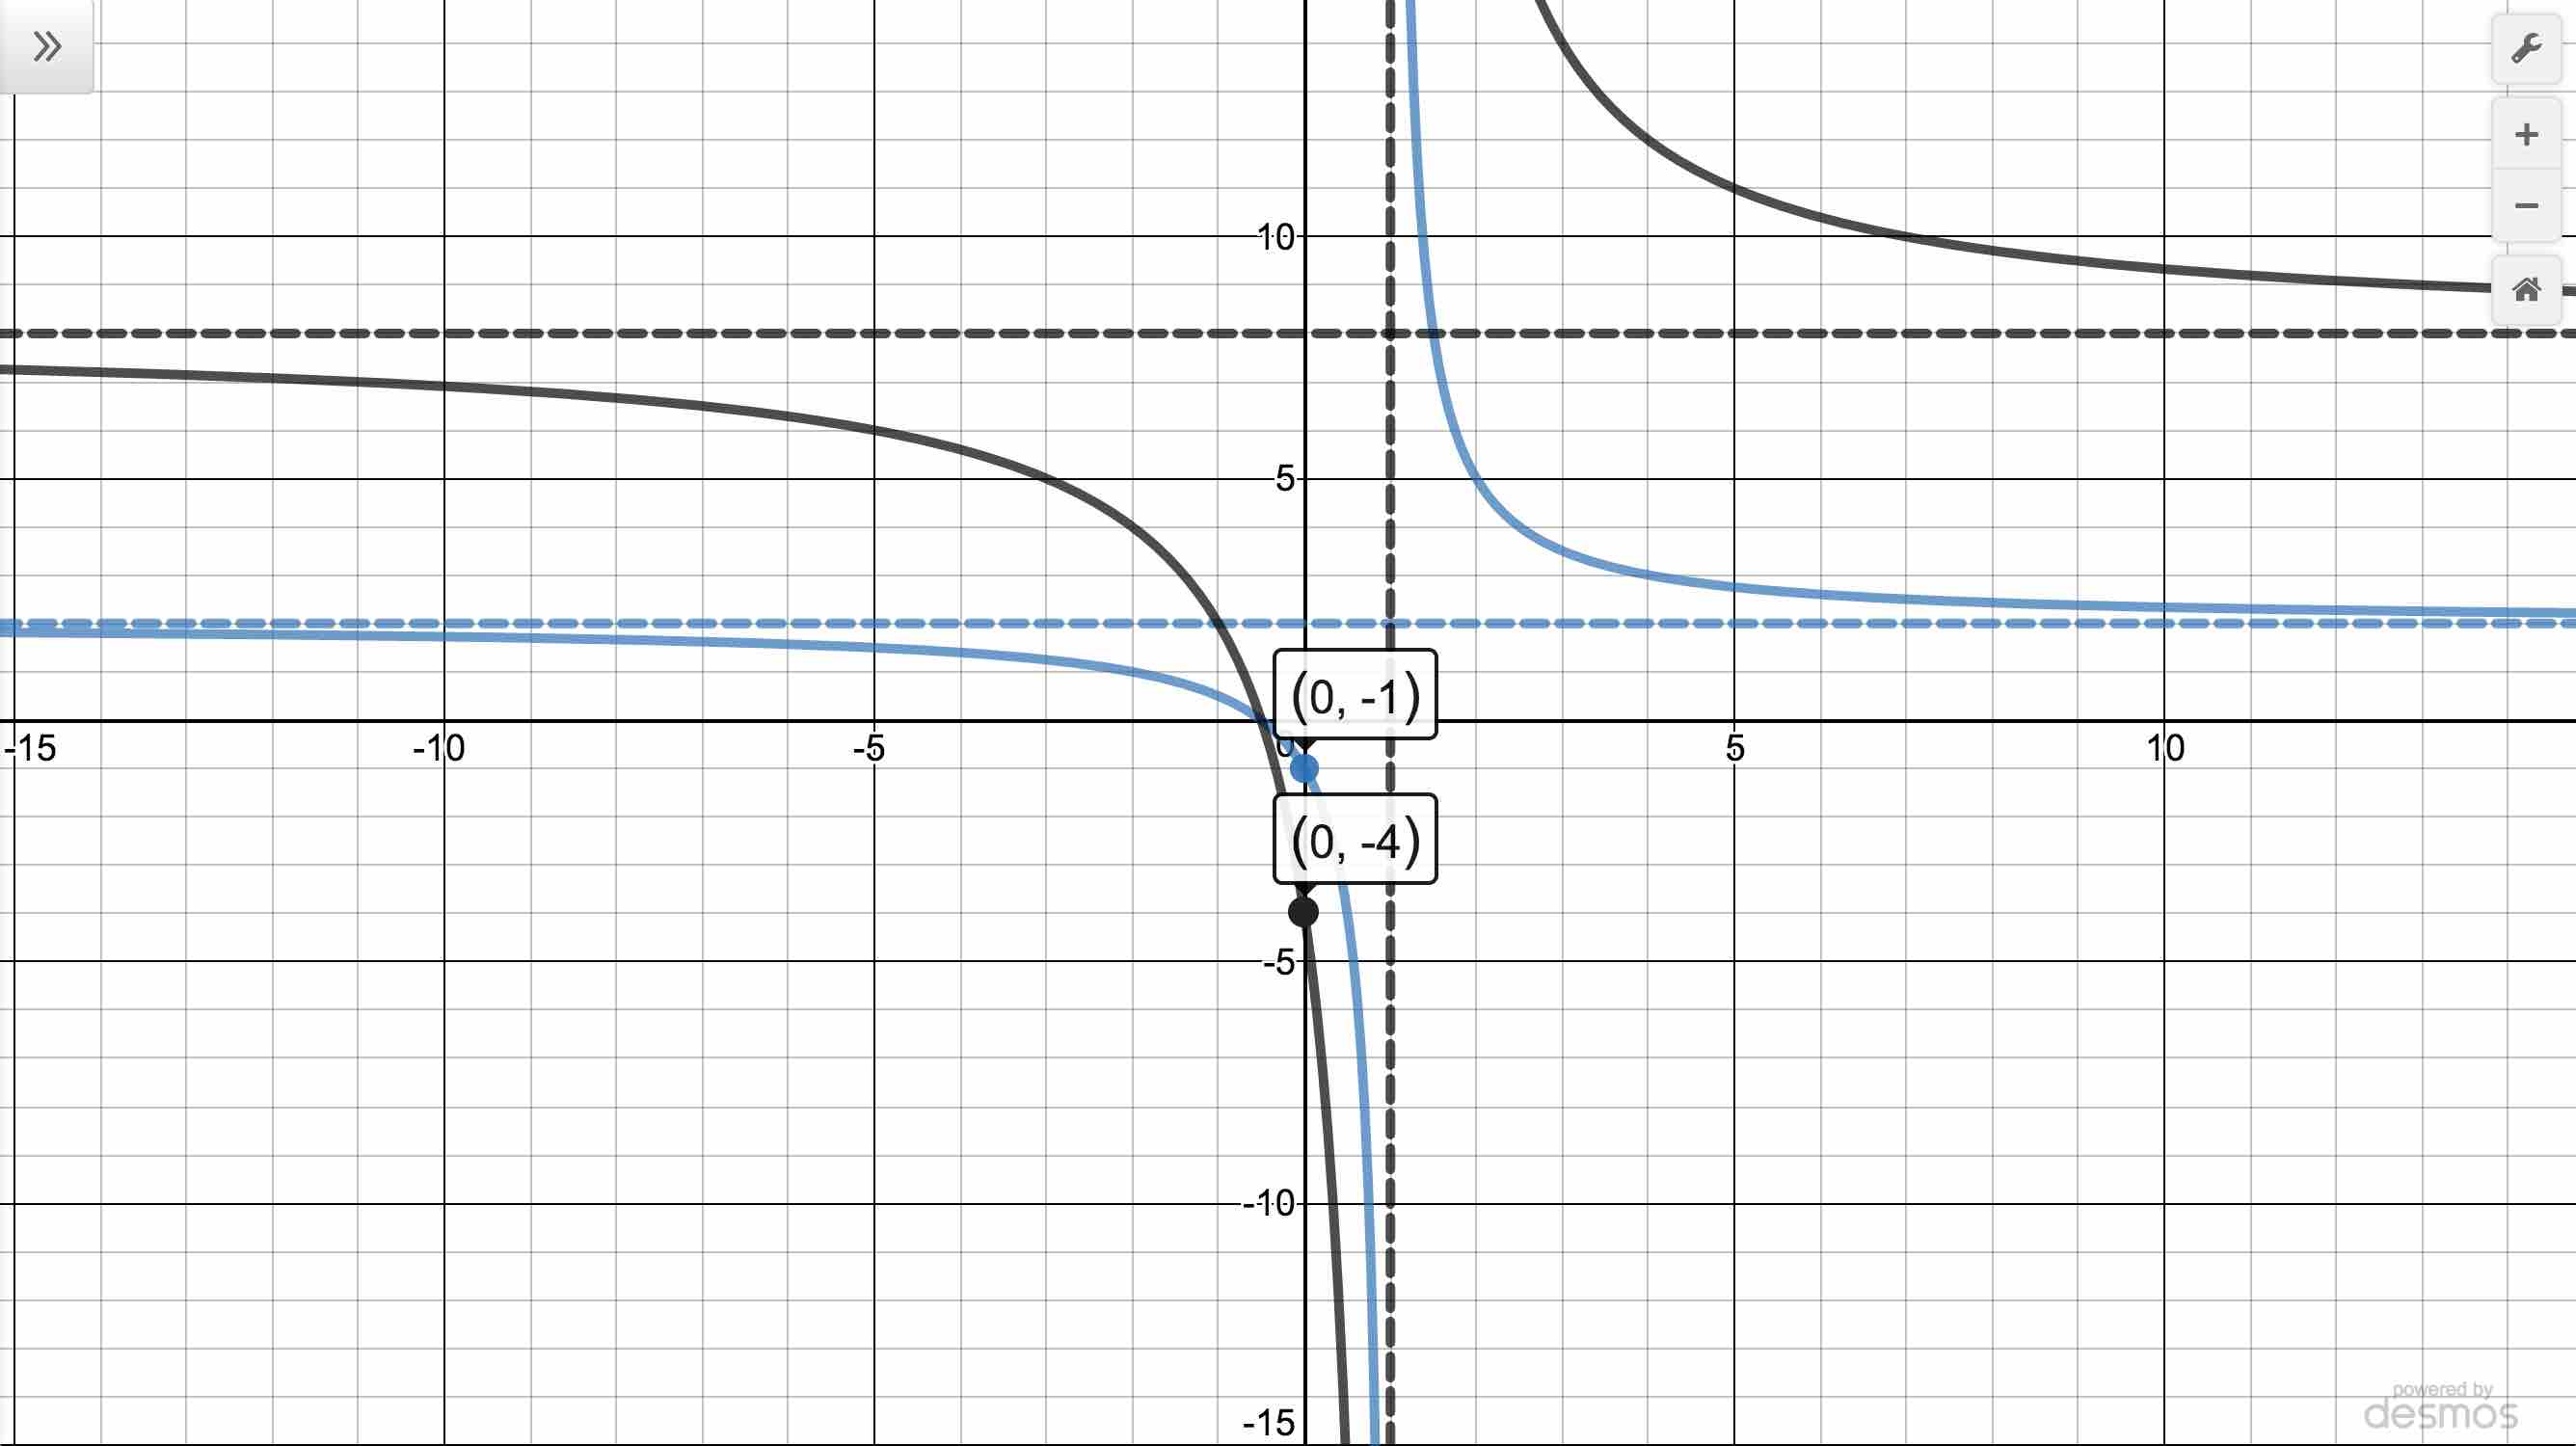
\includegraphics[width=3in]{./TransformationsGraphics/TransformationsEx03a.jpg} & 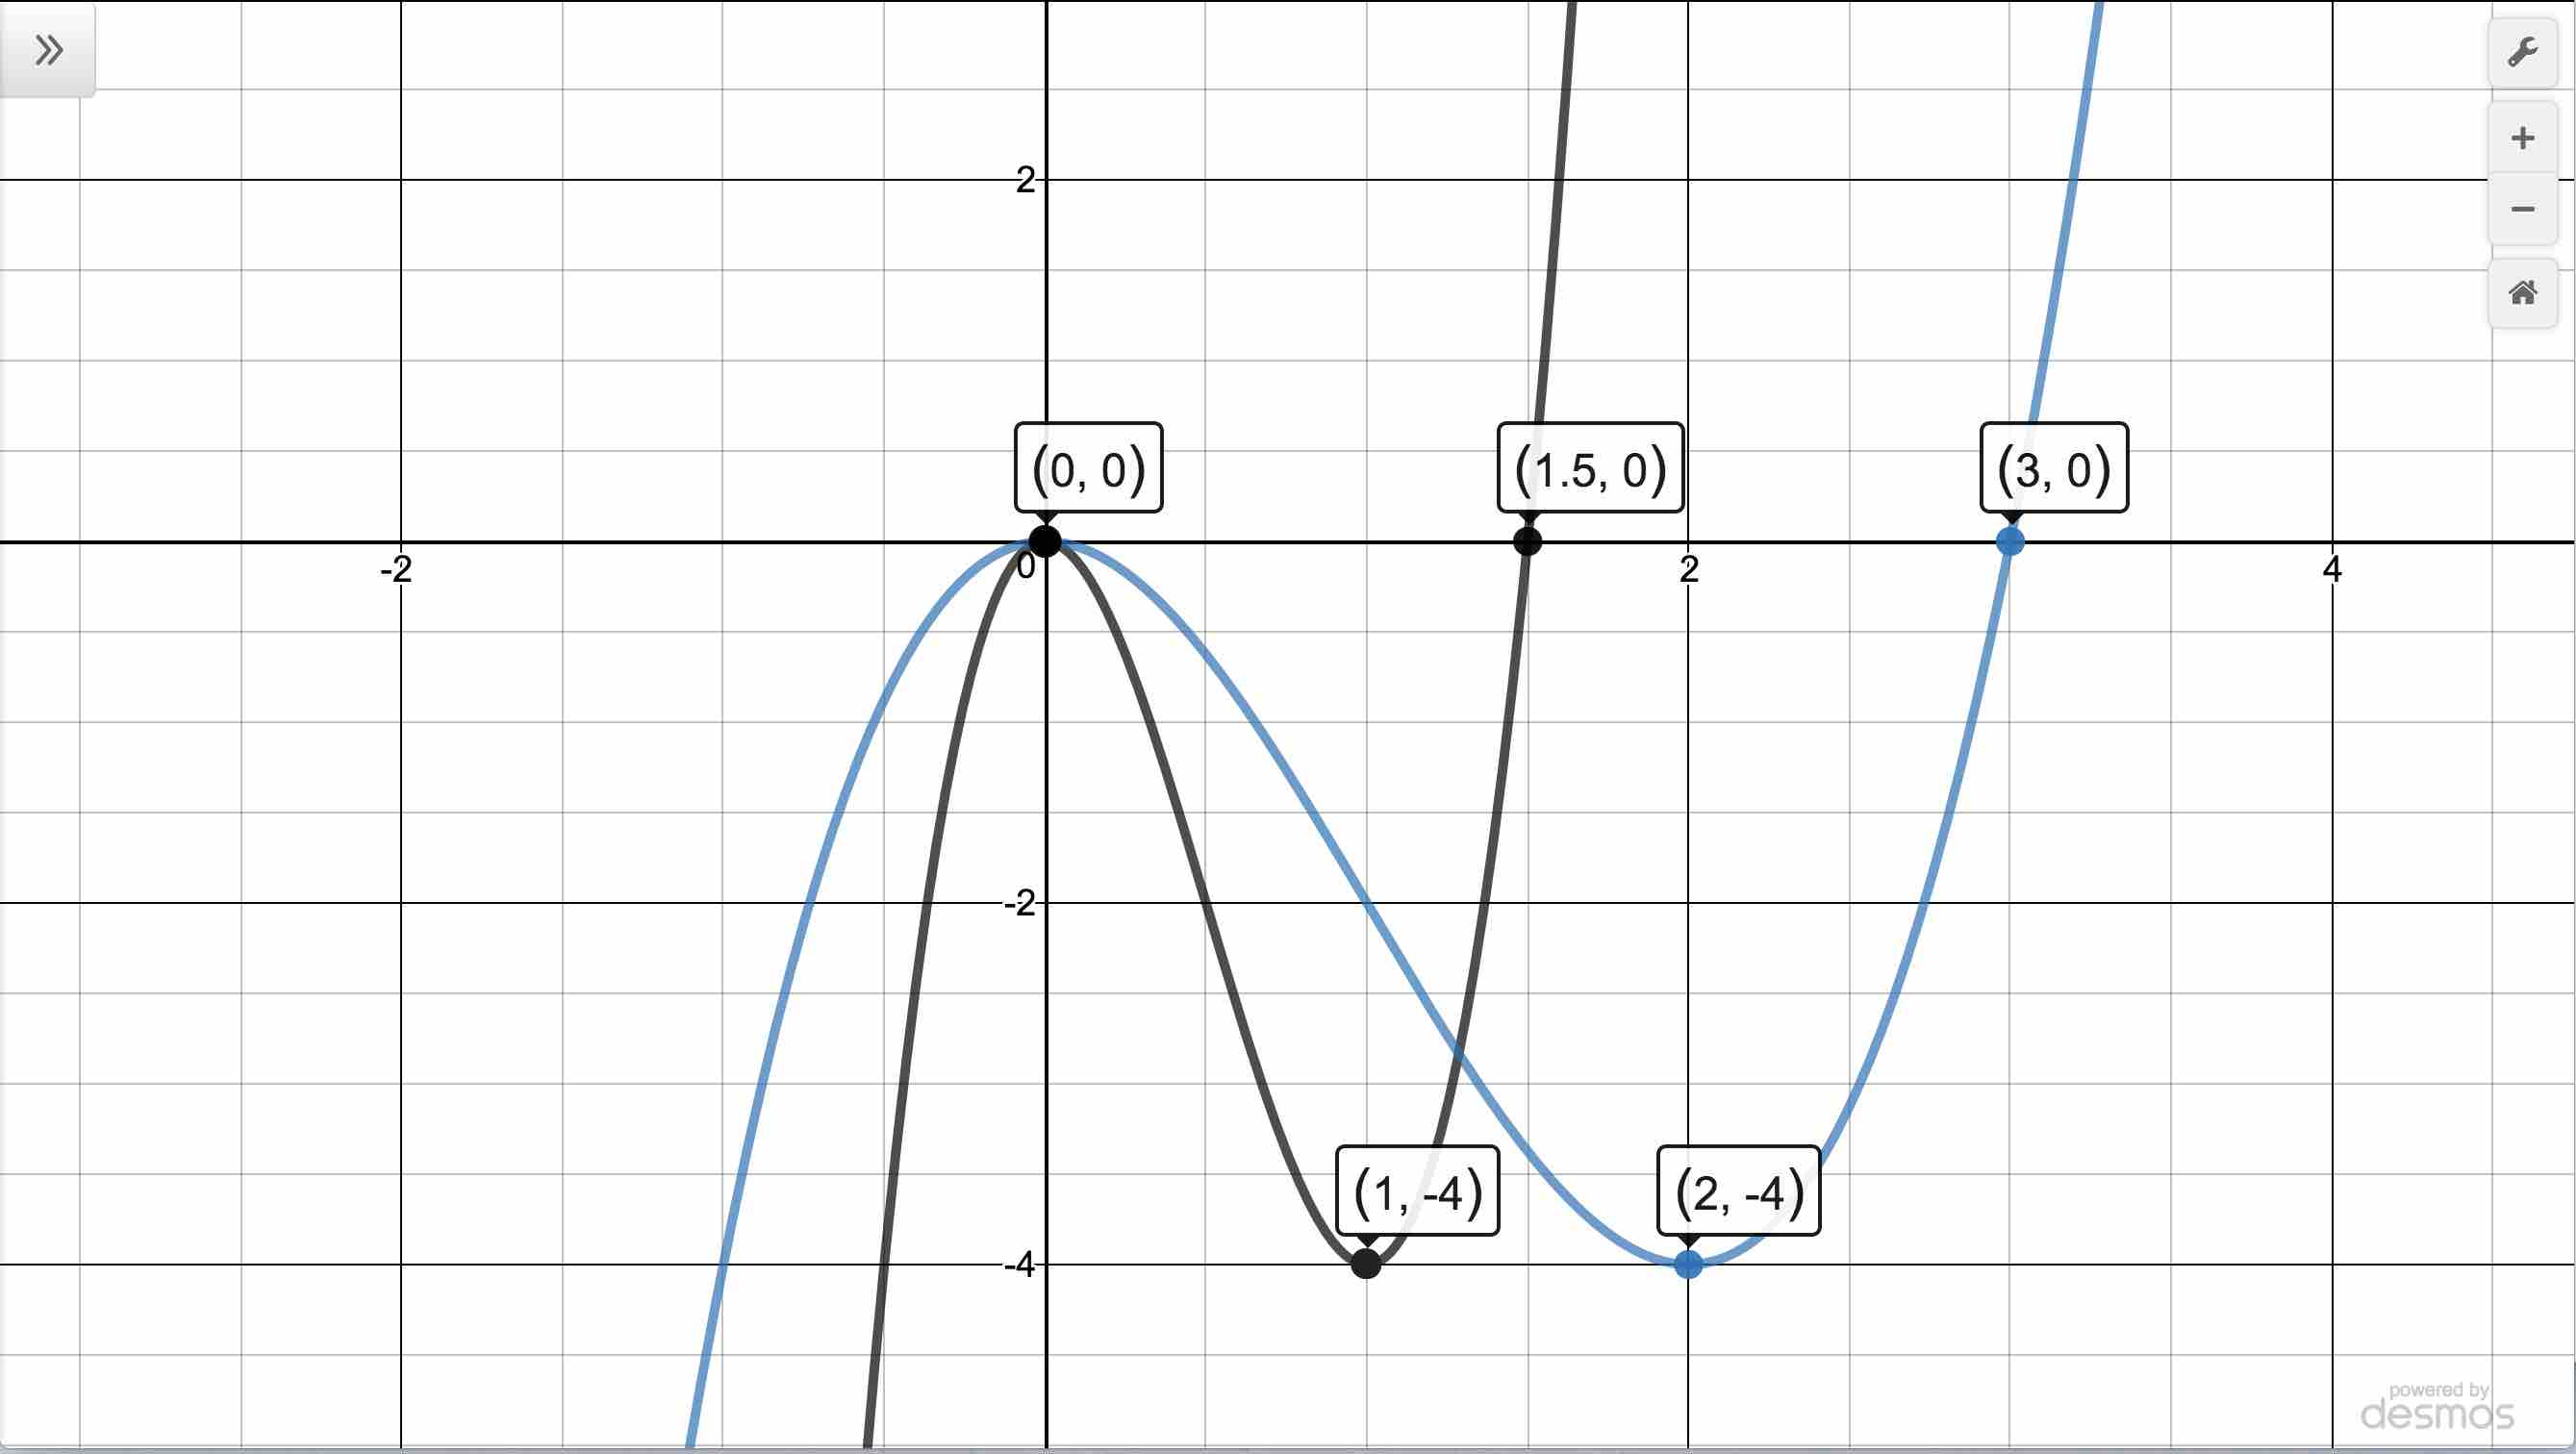
\includegraphics[width=3in]{./TransformationsGraphics/TransformationsEx03b.jpg} \\

{ \scriptsize $y=g(t) = \frac{2t+1}{t-1}$ (lighter color)  and $y=4g(t)=\dfrac{8t+4}{t-1}$}  &  {\scriptsize $y =  h(s) = s^3-3s^2$ (lighter color) and $y = H(s) = 8s^3 - 12s^2$} \\

\end{tabular}

\end{center} 
 
\item  

 
 \begin{enumerate}
 
 \item We first rewrite the expression for $F(x) = \frac{1-f(x)}{2} = -\frac{1}{2}f(x) + \frac{1}{2}$ in order to use the theorems available to us.  Note we have two modifications to the formula of $f(x)$ which correspond to three transformations.  
 
 \smallskip
 
 Multiplying $f(x)$ by $-\frac{1}{2}$ indicates a vertical compression by a factor of $2$ along with a reflection about the $x$-axis.  Adding $\frac{1}{2}$ indicates a vertical shift up $\frac{1}{2}$ units.  
 
 \smallskip
 
 As always the question is which to do first.  Once again, we look to algebra for the answer.  Picking the point $(1,0)$  on the graph of $f(x)$, we know $f(1) = 0$.  To see which point this corresponds to on the graph of $y=F(x)$, we find  $F(1) = -\frac{1}{2}f(1)+\frac{1}{2} = -\frac{1}{2} (0) +\frac{1}{2} = 0 + \frac{1}{2} = \frac{1}{2}$.  
 
 \smallskip
 
 Hence, we first multiplied the $y$-value $0$ by $-\frac{1}{2}$.  As above, we can think of $-\frac{1}{2} = (-1) \frac{1}{2}$  so that multiplying by $-\frac{1}{2}$ amounts to a vertical compression by a factor of $2$ first, then the refection about the $x$-axis second.  Lastly, adding the $\frac{1}{2}$ is the vertical shift up $\frac{1}{2}$ unit.  
 
 \smallskip
 
Beginning with the vertical scaling by a factor of $\frac{1}{2}$, we use Theorem \ref{vscalings} to graph $y=\frac{1}{2} f(x)$ starting from $y=f(x)$ by multiplying each of the $y$-coordinates of each of the points on the graph of $y=f(x)$ by $\frac{1}{2}$.
  


\[ \begin{array}{ccc}

\begin{mfpic}[15]{-1}{6}{-3}{3}
\axes
\tlabel[cc](6,-0.5){\scriptsize $x$}
\tlabel[cc](0.5,3){\scriptsize $y$}
\xmarks{ 0, 1, 2, 3,4,5}
\ymarks{-2, -1, 0, 1, 2}
\tcaption{\scriptsize $y = f(x)$}
\tlpointsep{4pt}
\scriptsize
\tlabel[cc](1.25, -0.75){$(1,0)$}
\tlabel[cc](2, 2){$(2,1)$}
\tlabel[cc](4, 2.75){$(4,2)$}
\axislabels {x}{{$2$} 2,{$3$} 3,{$4$} 4,{$5$} 5}
\axislabels {y}{{$-2$} -2,{$-1$} -1,{$1$} 1, {$2$} 2}
\normalsize
\penwd{1.25pt}
\arrow \reverse \arrow \parafcn{-2.5, 2.5, 0.1}{(2**t,t)}
\point[4pt]{(1,0), (2,1), (4,2)}
\end{mfpic}


&

\stackrel{\stackrel{\mbox{\scriptsize vertical scaling by a factor of $\frac{1}{2}$ }}{\xrightarrow{\hspace{1.7in}}}}{\mbox{ \scriptsize multiply each $y$-coordinate by $\frac{1}{2}$}} 

&

\begin{mfpic}[15]{-1}{6}{-3}{3}
\axes
\tlabel[cc](6,-0.5){\scriptsize $x$}
\tlabel[cc](0.5,3){\scriptsize $y$}
\xmarks{ 0, 1, 2, 3,4,5}
\ymarks{-2, -1, 0, 1, 2}
\tcaption{\scriptsize $y = \frac{1}{2}f(x)$}
\tlpointsep{4pt}
\scriptsize
\tlabel[cc](1, -0.75){$(1,0)$}
\tlabel[cc](2, 1.25){$\left(2, \frac{1}{2} \right)$}
\tlabel[cc](4, 1.5){$(4,1)$}
\axislabels {x}{{$2$} 2,{$3$} 3,{$4$} 4,{$5$} 5}
\axislabels {y}{{$-2$} -2,{$-1$} -1,{$1$} 1, {$2$} 2}
\normalsize
\penwd{1.25pt}
\arrow \reverse \arrow \parafcn{-3, 2.55, 0.1}{(2**t,t/2)}
\point[4pt]{(1,0), (2,0.5), (4,1)}
\end{mfpic} \\
 
\end{array} \]

Next, we reflect the graph of $y = \frac{1}{2} f(x)$ across the $x$-axis to produce the graph of $y=-\frac{1}{2} f(x)$ by multiplying each of the $y$-coordinates of the points on the graph of $y=\frac{1}{2} f(x)$ by $-1$:



\[ \begin{array}{ccc}

\begin{mfpic}[15]{-1}{6}{-3}{3}
\axes
\tlabel[cc](6,-0.5){\scriptsize $x$}
\tlabel[cc](0.5,3){\scriptsize $y$}
\xmarks{ 0, 1, 2, 3,4,5}
\ymarks{-2, -1, 0, 1, 2}
\tcaption{\scriptsize $y = \frac{1}{2}f(x)$}
\tlpointsep{4pt}
\scriptsize
\tlabel[cc](1, -0.75){$(1,0)$}
\tlabel[cc](2, 1.25){$\left(2, \frac{1}{2} \right)$}
\tlabel[cc](4, 1.5){$(4,1)$}
\axislabels {x}{{$2$} 2,{$3$} 3,{$4$} 4,{$5$} 5}
\axislabels {y}{{$-2$} -2,{$-1$} -1,{$1$} 1, {$2$} 2}
\normalsize
\penwd{1.25pt}
\arrow \reverse \arrow \parafcn{-3, 2.55, 0.1}{(2**t,t/2)}
\point[4pt]{(1,0), (2,0.5), (4,1)}
\end{mfpic}

&

\stackrel{\stackrel{\mbox{\scriptsize reflect about the $x$-axis }}{\xrightarrow{\hspace{1.7in}}}}{\mbox{ \scriptsize multiply each $y$-coordinate by $-1$}} 

&

\begin{mfpic}[15]{-1}{6}{-3}{3}
\axes
\tlabel[cc](6,-0.5){\scriptsize $x$}
\tlabel[cc](0.5,3){\scriptsize $y$}
\xmarks{ 0, 1, 2, 3,4,5}
\ymarks{-2, -1, 0, 1, 2}
\tcaption{\scriptsize $y = -\frac{1}{2}f(x)$}
\tlpointsep{4pt}
\scriptsize
\tlabel[cc](1.25, 0.5){$(1,0)$}
\tlabel[cc](2, -1.25){$\left(2, -\frac{1}{2} \right)$}
\tlabel[cc](4, -1.5){$(4,-1)$}
\axislabels {x}{{$3$} 3,{$4$} 4,{$5$} 5}
\axislabels {y}{{$-2$} -2,{$-1$} -1,{$1$} 1, {$2$} 2}
\normalsize
\penwd{1.25pt}
\arrow \reverse \arrow \parafcn{-3, 2.55, 0.1}{(2**t,-t/2)}
\point[4pt]{(1,0), (2,-0.5), (4,-1)}
\end{mfpic} \\
 
\end{array} \]

Finally, we shift the graph of $y = -\frac{1}{2} f(x)$ vertically up $\frac{1}{2}$ unit by adding $\frac{1}{2}$ to each of the $y$-coordinates of each of the points to obtain the graph of $y = -\frac{1}{2}f(x)+\frac{1}{2} = F(x)$.
 
 
\[ \begin{array}{ccc}

\begin{mfpic}[15]{-1}{6}{-3}{3}
\axes
\tlabel[cc](6,-0.5){\scriptsize $x$}
\tlabel[cc](0.5,3){\scriptsize $y$}
\xmarks{ 0, 1, 2, 3,4,5}
\ymarks{-2, -1, 0, 1, 2}
\tcaption{\scriptsize $y = -\frac{1}{2}f(x)$}
\tlpointsep{4pt}
\scriptsize
\tlabel[cc](1.25, 0.5){$(1,0)$}
\tlabel[cc](2, -1.25){$\left(2, -\frac{1}{2} \right)$}
\tlabel[cc](4, -1.5){$(4,-1)$}
\axislabels {x}{{$3$} 3,{$4$} 4,{$5$} 5}
\axislabels {y}{{$-2$} -2,{$-1$} -1,{$1$} 1, {$2$} 2}
\normalsize
\penwd{1.25pt}
\arrow \reverse \arrow \parafcn{-3, 2.55, 0.1}{(2**t,-t/2)}
\point[4pt]{(1,0), (2,-0.5), (4,-1)}
\end{mfpic} 
 


&

\stackrel{\stackrel{\mbox{\scriptsize shift up $\frac{1}{2}$ unit }}{\xrightarrow{\hspace{1.7in}}}}{\mbox{ \scriptsize add $\frac{1}{2}$ to each $y$-coordinate}} 

&

\begin{mfpic}[15]{-1}{6}{-3}{3}
\axes
\tlabel[cc](6,-0.5){\scriptsize $x$}
\tlabel[cc](0.5,3){\scriptsize $y$}
\xmarks{ 0, 1, 2, 3,4,5}
\ymarks{-2, -1, 0, 1, 2}
\tcaption{\scriptsize $y = -\frac{1}{2}f(x)+\frac{1}{2} = F(x)$}
\tlpointsep{4pt}
\scriptsize
\tlabel[cc](1.5, 1){$\left(1,\frac{1}{2} \right)$}
\tlabel[cc](2, -0.5){$(2,0)$}
\tlabel[cc](4, -1.25){$\left(4,-\frac{1}{2} \right)$}
\axislabels {x}{{$1$} 1,{$5$} 5}
\axislabels {y}{{$-2$} -2,{$-1$} -1,{$1$} 1, {$2$} 2}
\normalsize
\penwd{1.25pt}
\arrow \reverse \arrow \parafcn{-3, 2.55, 0.1}{(2**t,-t/2+0.5)}
\point[4pt]{(1,0.5), (2,0), (4,-0.5)}
\end{mfpic} \\
 
\end{array} \]

Note that as with horizontal scalings and reflections about the $y$-axis, the order of vertical scalings and reflections across the $x$-axis is interchangeable.  Had we decided to think of the factor $-\frac{1}{2} = \frac{1}{2} \cdot (-1)$, we could have just as well started with the graph of $y=f(x)$ and produced the graph of $y=-f(x)$ first:

\[ \begin{array}{ccc}

\begin{mfpic}[15]{-1}{6}{-3}{3}
\axes
\tlabel[cc](6,-0.5){\scriptsize $x$}
\tlabel[cc](0.5,3){\scriptsize $y$}
\xmarks{ 0, 1, 2, 3,4,5}
\ymarks{-2, -1, 0, 1, 2}
\tcaption{\scriptsize $y = f(x)$}
\tlpointsep{4pt}
\scriptsize
\tlabel[cc](1.25, -0.75){$(1,0)$}
\tlabel[cc](2, 2){$(2,1)$}
\tlabel[cc](4, 2.75){$(4,2)$}
\axislabels {x}{{$2$} 2,{$3$} 3,{$4$} 4,{$5$} 5}
\axislabels {y}{{$-2$} -2,{$-1$} -1,{$1$} 1, {$2$} 2}
\normalsize
\penwd{1.25pt}
\arrow \reverse \arrow \parafcn{-2.5, 2.5, 0.1}{(2**t,t)}
\point[4pt]{(1,0), (2,1), (4,2)}
\end{mfpic}


&

\stackrel{\stackrel{\mbox{\scriptsize reflect across the $x$-axis }}{\xrightarrow{\hspace{1.7in}}}}{\mbox{ \scriptsize multiply each $y$-coordinate by $-1$}} 

&

\begin{mfpic}[15]{-1}{6}{-3}{3}
\axes
\tlabel[cc](6,-0.5){\scriptsize $x$}
\tlabel[cc](0.5,3){\scriptsize $y$}
\xmarks{ 0, 1, 2, 3,4,5}
\ymarks{-2, -1, 0, 1, 2}
\tcaption{\scriptsize $y = -f(x)$}
\tlpointsep{4pt}
\scriptsize
\tlabel[cc](1.5, 0.5){$(1,0)$}
\tlabel[cc](2, -1.75){$(2,-1)$}
\tlabel[cc](4, -2.75){$(4,-2)$}
\axislabels {x}{{$2$} 2,{$3$} 3,{$4$} 4,{$5$} 5}
\axislabels {y}{{$-2$} -2,{$-1$} -1,{$1$} 1, {$2$} 2}
\normalsize
\penwd{1.25pt}
\arrow \reverse \arrow \parafcn{-2.5, 2.5, 0.1}{(2**t,-t)}
\point[4pt]{(1,0), (2,-1), (4,-2)}
\end{mfpic} \\
 
\end{array} \]

Next, we vertically scale the graph of $y=-f(x)$  by multiplying each of the $y$-coordinates of each of the points on the graph of $y=-f(x)$ by $\frac{1}{2}$ to obtain the graph of $y = -\frac{1}{2} f(x)$:

 
 
 \[ \begin{array}{ccc}

\begin{mfpic}[15]{-1}{6}{-3}{3}
\axes
\tlabel[cc](6,-0.5){\scriptsize $x$}
\tlabel[cc](0.5,3){\scriptsize $y$}
\xmarks{ 0, 1, 2, 3,4,5}
\ymarks{-2, -1, 0, 1, 2}
\tcaption{\scriptsize $y = -f(x)$}
\tlpointsep{4pt}
\scriptsize
\tlabel[cc](1, -1){$(1,0)$}
\tlabel[cc](2, -2){$(2,-1)$}
\tlabel[cc](4, -2.75){$(4,-2)$}
\axislabels {x}{{$2$} 2,{$3$} 3,{$4$} 4,{$5$} 5}
\axislabels {y}{{$-2$} -2,{$-1$} -1,{$1$} 1, {$2$} 2}
\normalsize
\penwd{1.25pt}
\arrow \reverse \arrow \parafcn{-2.5, 2.5, 0.1}{(2**t,-t)}
\point[4pt]{(1,0), (2,-1), (4,-2)}
\end{mfpic}

&

\stackrel{\stackrel{\mbox{\scriptsize vertical scaling by a factor of $\frac{1}{2}$ }}{\xrightarrow{\hspace{1.7in}}}}{\mbox{ \scriptsize multiply each $y$-coordinate by $\frac{1}{2}$}} 

&

\begin{mfpic}[15]{-1}{6}{-3}{3}
\axes
\tlabel[cc](6,-0.5){\scriptsize $x$}
\tlabel[cc](0.5,3){\scriptsize $y$}
\xmarks{ 0, 1, 2, 3,4,5}
\ymarks{-2, -1, 0, 1, 2}
\tcaption{\scriptsize $y = -\frac{1}{2}f(x)$}
\tlpointsep{4pt}
\scriptsize
\tlabel[cc](1.25, 0.5){$(1,0)$}
\tlabel[cc](2, -1.25){$\left(2, -\frac{1}{2} \right)$}
\tlabel[cc](4, -1.5){$(4,-1)$}
\axislabels {x}{{$3$} 3,{$4$} 4,{$5$} 5}
\axislabels {y}{{$-2$} -2,{$-1$} -1,{$1$} 1, {$2$} 2}
\normalsize
\penwd{1.25pt}
\arrow \reverse \arrow \parafcn{-3, 2.55, 0.1}{(2**t,-t/2)}
\point[4pt]{(1,0), (2,-0.5), (4,-1)}
\end{mfpic} \\
 
\end{array} \]


Notice we've reached the same graph of $y=-\frac{1}{2} f(x)$ that we had before, and, hence we arrive at the same final answer as before:

\[ \begin{array}{ccc}

\begin{mfpic}[15]{-1}{6}{-3}{3}
\axes
\tlabel[cc](6,-0.5){\scriptsize $x$}
\tlabel[cc](0.5,3){\scriptsize $y$}
\xmarks{ 0, 1, 2, 3,4,5}
\ymarks{-2, -1, 0, 1, 2}
\tcaption{\scriptsize $y = -\frac{1}{2}f(x)$}
\tlpointsep{4pt}
\scriptsize
\tlabel[cc](1.25, 0.5){$(1,0)$}
\tlabel[cc](2, -1.25){$\left(2, -\frac{1}{2} \right)$}
\tlabel[cc](4, -1.5){$(4,-1)$}
\axislabels {x}{{$3$} 3,{$4$} 4,{$5$} 5}
\axislabels {y}{{$-2$} -2,{$-1$} -1,{$1$} 1, {$2$} 2}
\normalsize
\penwd{1.25pt}
\arrow \reverse \arrow \parafcn{-3, 2.55, 0.1}{(2**t,-t/2)}
\point[4pt]{(1,0), (2,-0.5), (4,-1)}
\end{mfpic} 
 


&

\stackrel{\stackrel{\mbox{\scriptsize shift up $\frac{1}{2}$ unit }}{\xrightarrow{\hspace{1.7in}}}}{\mbox{ \scriptsize add $\frac{1}{2}$ to each $y$-coordinate}} 

&

\begin{mfpic}[15]{-1}{6}{-3}{3}
\axes
\tlabel[cc](6,-0.5){\scriptsize $x$}
\tlabel[cc](0.5,3){\scriptsize $y$}
\xmarks{ 0, 1, 2, 3,4,5}
\ymarks{-2, -1, 0, 1, 2}
\tcaption{\scriptsize $y = -\frac{1}{2}f(x)+\frac{1}{2} = F(x)$}
\tlpointsep{4pt}
\scriptsize
\tlabel[cc](1.5, 1){$\left(1,\frac{1}{2} \right)$}
\tlabel[cc](2, -0.5){$(2,0)$}
\tlabel[cc](4, -1.25){$\left(4,-\frac{1}{2} \right)$}
\axislabels {x}{{$1$} 1,{$5$} 5}
\axislabels {y}{{$-2$} -2,{$-1$} -1,{$1$} 1, {$2$} 2}
\normalsize
\penwd{1.25pt}
\arrow \reverse \arrow \parafcn{-3, 2.55, 0.1}{(2**t,-t/2+0.5)}
\point[4pt]{(1,0.5), (2,0), (4,-0.5)}
\end{mfpic} \\
 
\end{array} \]

We check our answer as we have so many times before.  We start with the point $\left(1, \frac{1}{2}\right)$ and substitute $x=1$ into $y=\frac{1-f(x)}{2}$ to get $y=\frac{1-f(1)}{2}$.  From the graph of $f$, we know $f(1) = 0$, so we get $y=\frac{1-f(1)}{2} = \frac{1-0}{2} = \frac{1}{2}$.  This proves $\left(1, \frac{1}{2}\right)$ is on the graph of $y=\frac{1-f(x)}{2}$.  We invite the reader to check the remaining points.


Note that in the preceding example, since none of the transformations included adjusting the $x$-coordinates of points, the vertical asymptote, $x=0$ remained in place.

 
  \item  As with the previous example, we first rewrite $F(x)= f\left( \frac{1-x}{2} \right) = F\left( -\frac{1}{2}x + \frac{1}{2} \right)$.  Here again, we have two modifications to the formula $f(x)$, the $-\frac{1}{2}$ multiple indicating a horizontal scaling and a reflection across the $y$-axis and a horizontal shift. 
  
  \smallskip
  
   Based on our experience from previous examples, we do the horizontal shift first, with the order of the scaling and reflection more or less irrelevant.   
  
  \smallskip
  
  To  produce the graph of $y = f\left(x+\frac{1}{2}\right)$ we subtract $\frac{1}{2}$ from each of the $x$-coordinates of each of the points on the graph of $y=f(x)$.  This moves the graph to the left $\frac{1}{2}$ unit, including the vertical asymptote $x=0$ which moves to $x = -\frac{1}{2}$.
  
\[ \begin{array}{ccc}

\begin{mfpic}[15]{-1}{6}{-3}{3}
\axes
\tlabel[cc](6,-0.5){\scriptsize $x$}
\tlabel[cc](0.5,3){\scriptsize $y$}
\xmarks{ 0, 1, 2, 3,4,5}
\ymarks{-2, -1, 0, 1, 2}
\tcaption{\scriptsize $y = f(x)$}
\tlpointsep{4pt}
\scriptsize
\tlabel[cc](1.25, -0.75){$(1,0)$}
\tlabel[cc](2, 2){$(2,1)$}
\tlabel[cc](4, 2.75){$(4,2)$}
\axislabels {x}{{$2$} 2,{$3$} 3,{$4$} 4,{$5$} 5}
\axislabels {y}{{$-2$} -2,{$-1$} -1,{$1$} 1, {$2$} 2}
\normalsize
\penwd{1.25pt}
\arrow \reverse \arrow \parafcn{-2.5, 2.5, 0.1}{(2**t,t)}
\point[4pt]{(1,0), (2,1), (4,2)}
\end{mfpic}


&

\stackrel{\stackrel{\mbox{\scriptsize shift left $\frac{1}{2}$ unit }}{\xrightarrow{\hspace{1.7in}}}}{\mbox{ \scriptsize subtract $\frac{1}{2}$ from each $x$-coordinate}} 

&

\begin{mfpic}[15]{-2}{5}{-3}{3}
\axes
\tlabel[cc](5,-0.5){\scriptsize $x$}
\tlabel[cc](0.5,3){\scriptsize $y$}
\xmarks{ -1, 0, 1, 2, 3,4}
\ymarks{-2, -1, 0, 1, 2}
\tcaption{\scriptsize $y = f\left(x + \frac{1}{2} \right)$}
\tlpointsep{4pt}
\scriptsize
\tlabel[cc](1, -0.75){$\left( \frac{1}{2} ,0 \right)$}
\tlabel[cc](1.25, 1.75){$\left( \frac{3}{2} ,1\right)$}
\tlabel[cc](3.25, 2.5){$\left(\frac{7}{2},2 \right)$}
\axislabels {x}{{$-1 \hspace{7pt}$} -1, {$2$} 2,{$3$} 3,{$4$} 4}
\axislabels {y}{{$1$} 1,{ $2$} 2}
\normalsize
\dashed \polyline{(-0.5, -3), (-0.5, 3)}
\tlabel[cc](-1.5, -2.5){\scriptsize $x=-\frac{1}{2}$}
\penwd{1.25pt}
\arrow \reverse \arrow \parafcn{-2.5, 2.5, 0.1}{((2**t) - 0.5,t)}
\point[4pt]{(0.5,0), (1.5,1), (3.5,2)}
\end{mfpic} \\
 
\end{array} \]


Next, we graph $y = f\left(\frac{1}{2}x + \frac{1}{2} \right)$ starting with $y = f\left(x+\frac{1}{2}\right)$ by horizontally expanding the graph by a factor of $2$.  That is, we multiply each $x$-coordinates on the graph of $y = f\left(x+\frac{1}{2}\right)$  by $2$, including the vertical asymptote, $x  =-\frac{1}{2}$ which moves to $x = 2 \left(-\frac{1}{2} \right) = -1$.


\[ \begin{array}{ccc}

\begin{mfpic}[15]{-2}{5}{-3}{3}
\axes
\tlabel[cc](5,-0.5){\scriptsize $x$}
\tlabel[cc](0.5,3){\scriptsize $y$}
\xmarks{ -1, 0, 1, 2, 3,4}
\ymarks{-2, -1, 0, 1, 2}
\tcaption{\scriptsize $y = f\left(x + \frac{1}{2} \right)$}
\tlpointsep{4pt}
\scriptsize
\tlabel[cc](1, -0.75){$\left( \frac{1}{2} ,0 \right)$}
\tlabel[cc](1.25, 1.75){$\left( \frac{3}{2} ,1\right)$}
\tlabel[cc](3.25, 2.5){$\left(\frac{7}{2},2 \right)$}
\axislabels {x}{{$-1 \hspace{7pt}$} -1, {$2$} 2,{$3$} 3,{$4$} 4}
\axislabels {y}{{$1$} 1,{ $2$} 2}
\normalsize
\dashed \polyline{(-0.5, -3), (-0.5, 3)}
\tlabel[cc](-1.5, -2.5){\scriptsize $x=-\frac{1}{2}$}
\penwd{1.25pt}
\arrow \reverse \arrow \parafcn{-2.5, 2.5, 0.1}{((2**t) - 0.5,t)}
\point[4pt]{(0.5,0), (1.5,1), (3.5,2)}
\end{mfpic}


&

\stackrel{\stackrel{\mbox{\scriptsize horizontal scaling by a factor of $2$ }}{\xrightarrow{\hspace{1.7in}}}}{\mbox{ \scriptsize multiply eac $x$-coordinate by $2$}} 

&

\begin{mfpic}[11][15]{-2}{10}{-3}{3}
\axes
\tlabel[cc](10,-0.5){\scriptsize $x$}
\tlabel[cc](0.5,3){\scriptsize $y$}
\xmarks{-2, -1, 0, 1, 2, 3,4,5,6,7,8,9}
\ymarks{-2, -1, 0, 1, 2}
\tcaption{\scriptsize $y = f\left(\frac{1}{2}x + \frac{1}{2} \right)$}
\tlpointsep{4pt}
\scriptsize
\tlabel[cc](0.75, 0.5){$(1,0)$}
\tlabel[cc](3, 1.5){$(3,1)$}
\tlabel[cc](7, 2.5){$(7,2)$}
\axislabels {x}{{$-2 \hspace{7pt}$} -2, ,{$1$} 1, {$2$} 2,{$3$} 3,{$4$} 4,{$5$} 5,{$6$} 6,{$7$} 7,{$8$} 8,{$9$} 9}
\axislabels {y}{{$1$} 1,{ $2$} 2}
\normalsize
\dashed \polyline{(-1, -3), (-1, 3)}
\tlabel[cc](-2.5, -2.5){\scriptsize $x=-1$}
\penwd{1.25pt}
\arrow \reverse \arrow \parafcn{-2.5, 2.4, 0.1}{(   2*((2**t) - 0.5),t)}
\point[4pt]{(1,0), (3,1), (7,2)}
\end{mfpic} \\
 
\end{array} \]

Finally, we reflect the graph of $y = f\left(\frac{1}{2}x + \frac{1}{2} \right)$ about the $y$-axis to graph $y = f\left(-\frac{1}{2}x + \frac{1}{2} \right)$. We accomplish this by multiplying each of the $x$-coordinates of each of the points on the graph of  $y = f\left(\frac{1}{2}x + \frac{1}{2} \right)$ by $-1$.  This includes the vertical asymptote which is moved to $x = (-1)(-1) = 1$.


 \[ \begin{array}{ccc}

\begin{mfpic}[11][15]{-2}{10}{-3}{3}
\axes
\tlabel[cc](10,-0.5){\scriptsize $x$}
\tlabel[cc](0.5,3){\scriptsize $y$}
\xmarks{-2, -1, 0, 1, 2, 3,4,5,6,7,8,9}
\ymarks{-2, -1, 0, 1, 2}
\tcaption{\scriptsize $y = f\left(\frac{1}{2}x + \frac{1}{2} \right)$}
\tlpointsep{4pt}
\scriptsize
\tlabel[cc](0.75, 0.5){$(1,0)$}
\tlabel[cc](3, 1.5){$(3,1)$}
\tlabel[cc](7, 2.5){$(7,2)$}
\axislabels {x}{{$-2 \hspace{7pt}$} -2, ,{$1$} 1, {$2$} 2,{$3$} 3,{$4$} 4,{$5$} 5,{$6$} 6,{$7$} 7,{$8$} 8,{$9$} 9}
\axislabels {y}{{$1$} 1,{ $2$} 2}
\normalsize
\dashed \polyline{(-1, -3), (-1, 3)}
\tlabel[cc](-2.5, -2.5){\scriptsize $x=-1$}
\penwd{1.25pt}
\arrow \reverse \arrow \parafcn{-2.5, 2.4, 0.1}{(   2*((2**t) - 0.5),t)}
\point[4pt]{(1,0), (3,1), (7,2)}
\end{mfpic}


&

\stackrel{\stackrel{\mbox{\scriptsize horizontal scaling by a factor of $2$ }}{\xrightarrow{\hspace{1.7in}}}}{\mbox{ \scriptsize multiply each $x$-coordinate by $2$}} 

&

\begin{mfpic}[11][15]{-10}{2}{-3}{3}
\axes
\tlabel[cc](2,-0.5){\scriptsize $x$}
\tlabel[cc](0.5,3){\scriptsize $y$}
\xmarks{1, 0, -1, -2, -3,-4,-5,-6,-7,-8,-9}
\ymarks{-2, -1, 0, 1, 2}
\tcaption{\scriptsize $y = f\left(-\frac{1}{2}x + \frac{1}{2} \right)$}
\tlpointsep{4pt}
\scriptsize
\tlabel[cc](-1.5, -0.75){$(-1,0)$}
\tlabel[cc](-2.75, 1.5){$(-3,1)$}
\tlabel[cc](-7, 2.5){$(-7,2)$}
\axislabels {x}{  {$-3 \hspace{7pt}$} -3,  {$-5 \hspace{7pt}$} -5, {$-7 \hspace{7pt}$} -7, {$-9 \hspace{7pt}$} -9}
\axislabels {y}{{$1$} 1,{ $2$} 2}
\normalsize
\dashed \polyline{(1, -3), (1, 3)}
\tlabel[cc](2.5, -2.5){\scriptsize $x=1$}
\penwd{1.25pt}
\arrow \reverse \arrow \parafcn{-2.5, 2.4, 0.1}{(  0 - (2* ( (2**t) - 0.5)  ),  t  )}


\point[4pt]{(-1,0), (-3,1), (-7,2)}
\end{mfpic} \\
 
\end{array} \]

To check our answer, we begin with the point $(-1,0)$ and substitute $x=-1$ into $y = f\left( \frac{1-x}{2} \right)$.  We get $y = f\left( \frac{1-(-1)}{2} \right) = f\left( \frac{2}{2} \right) = f(1)$.  From the graph of $f$, we know $f(1) = 0$, hence we have $y = f(1) = 0$, proving $(-1,0)$ is on the graph of $y = f\left( \frac{1-x}{2}\right)$.  The reader is encouraged to check the remaining points.


As mentioned previously, instead of doing the horizontal scaling first, then the reflection, we could have done the reflection first, then the scaling.  We leave this to the reader to check.

 \end{enumerate}

 
 \item To write $g(x)$ in terms of $f(x)$, we assume we can find real numbers $a$, $b$, $h$, and $k$ and choose signs $\pm$ so that $g(x) = \pm a f(\pm b x - h)+k$.   
 
 \smallskip
 
 The most notable change we see is the vertical asymptote $x=0$ has moved to $x=2$.  Moreover, instead of the graph increasing off to the right, it is decreasing coming in from the left.  This suggests a horizontal shift of $2$ units as well as a reflection across the $y$-axis.  
 
 \smallskip
 
 Since we always shift first then reflect, we have a shift \textit{left} of $2$ units followed by a reflection about the $y$-axis.  In other words, $g(x) = \pm a f(-x+2) + k$.  
 
 \smallskip
 
 Comparing $y$-values, the $y$-values on the graph of $g$ appear to be exactly twice the corresponding values on the graph of $f$, indicating a vertical stretch by a factor of $2$.  Hence, we get $g(x) = 2 f(-x+2)$.  We leave it to the reader to check the graph of $y=2f(-x+2)$ matches the graph of $y=g(x)$.  
 
 \smallskip
 
To write $f(x)$ in terms of $g(x)$, we reverse the steps done in obtaining the graph of $g(x)$ from $f(x)$ in the reverse order.  

\smallskip

Since to get from the graph of $f$ to the graph of $g$, we: first, shifted left $2$ units; second reflected across the $y$-axis; third, vertically stretched by a factor of $2$, our first step in taking $g$ back to $f$ is to implement a vertical compression by a factor of $2$.  Hence, starting with the graph of $y=g(x)$, our first step results in the formula $y = \frac{1}{2} g(x)$. 

\smallskip

 Next, we need to undo the reflection abut the $y$-axis.  If the point $(a,b)$ is reflected about the $y$-axis, we obtain the point $(-a,b)$.  To return to the point $(a,b)$, we reflect $(-a,b)$ across the $y$-axis again: $(-(-a),b) = (a,b)$.  Hence, we take the graph of $y = \frac{1}{2} g(x)$ and reflect it across the $y$-axis to obtain $y = \frac{1}{2} g(-x)$.  
 
 \smallskip
 
 Our last step is to undo a horizontal shift to the left $2$ units.  The reverse of this process is shifting the graph to the \textit{right} two units, so we get $y = \frac{1}{2} g(-(x-2)) = \frac{1}{2} g(-x+2)$.\footnote{To see this better, let $F(x) = \frac{1}{2} g(-x)$.  Per Theorem \ref{hshifts}, the graph of  $F(x-2) = \frac{1}{2} g(-(x-2)) = \frac{1}{2} g(-x+2)$ is the same as the graph of $F$ but shifted $2$ units to the right.}  
 
 \smallskip
 
 We leave it to the reader to start with the graph of $y=g(x)$ and check the graph of $y =  \frac{1}{2} g(-x+2)$ matches the graph of $y = f(x)$. \qed

\end{enumerate}

\end{ex}

\subsection{Transformations in Sequence}
\label{TransformationsinSequence}


Now that we have studied  three basic classes of transformations:  shifts, reflections, and scalings, we present a result below which provides one algorithm to follow to transform the graph of $y=f(x)$ into the graph of $y=af(bx-h)+k$ without the need of using Theorems \ref{vshifts}, \ref{hshifts}, \ref{reflections}, \ref{vscalings} and \ref{hscalings} individually.  

\smallskip

Theorem \ref{transformationsthm} is the ultimate generalization of Theorems \ref{linearabsvaluegraphs}, \ref{standardformgraph}, \ref{linearmononialgraphs},  \ref{linearlaurentlgraphs}, \ref{linearrootgraphs} and \ref{linearrationalpowergraphs}.  We note the underlying assumption here is that regardless of the order or number of shifts, reflections and scalings applied to the graph of a function $f$, we can always represent the final result in the form $g(x) = a f(bx-h)+k$.   Since each of these transformations can ultimately be traced back to composing $f$ with linear functions,\footnote{See the remarks at the beginning of the section.} this fact is verified by showing compositions of linear functions results in a linear function.\footnote{See Exercise \ref{CompLinearisLinearExercise}.}

\smallskip

\colorbox{ResultColor}{\bbm

%\smallskip

\begin{thm} \label{transformationsthm}\index{transformations of function graphs}\index{function ! transformation of graphs}\index{graph ! transformations}\textbf{Transformations in Sequence.}  Suppose $f$ is a function.  If $a, b \neq 0$, then to graph $g(x) = a f(bx-h)+k$ start with the graph of $y=f(x)$ and follow the steps below.

\begin{enumerate}

\item  Add $h$ to each of the $x$-coordinates of the points on the graph of $f$.  

\textbf{NOTE:} This results in a horizontal shift to the left if $h < 0$ or right if $h > 0$.

\item  Divide the $x$-coordinates of the points on the graph obtained in Step 1 by $b$.  

\textbf{NOTE:} This results in a horizontal scaling, but includes a reflection about the $y$-axis if $b < 0$.

\item  Multiply the $y$-coordinates of the points on the graph obtained in Step 2 by $a$.   

\textbf{NOTE:} This results in a vertical scaling, but  includes a reflection about the $x$-axis if $a < 0$.

\item  Add $k$ to each of the $y$-coordinates of the points on the graph obtained in Step 3.  

\textbf{NOTE:} This results in a vertical shift up if $k > 0$ or down if $k < 0$.

\end{enumerate}

\end{thm}

\ebm}

\bigskip

Theorem \ref{transformationsthm} can be established by generalizing the techniques developed in this section.  Suppose $(c,f(c))$ is on the graph of $f$. To match up the inputs of $f(bx-h)$ and $f(c)$, we solve $bx-h = c$ and solve.  

\smallskip

We first add the $h$ (causing the horizontal shift) and then divide by $b$.  If $b$ is a positive number, this induces only a horizontal scaling by a factor of $\frac{1}{b}$.  If  $b<0$, then we have a factor of $-1$ in play, and dividing by it induces a reflection about the $y$-axis.  So we have $x = \frac{c+h}{b}$ as the input to $g$ which corresponds to the input $x=c$ to $f$.  

\smallskip

We now evaluate $g\left( \frac{c+h}{b}\right) = a f\left(b \cdot \frac{c+h}{b} -h \right) + K = a f(c+h-h) =  a f(c)+k$.  We notice that the output from $f$ is first multiplied by $a$.  As with the constant $b$, if $a > 0$, this induces only a vertical scaling.  If $a < 0$, then the $-1$ induces a reflection across the $x$-axis.  Finally, we add $k$ to the result, which is our vertical shift.  

\smallskip

A less precise, but more intuitive way to paraphrase Theorem \ref{transformationsthm} is to think of the quantity $bx-h$ is the `inside' of the function $f$.  What's happening inside $f$ affects the inputs or $x$-coordinates of the points on the graph of $f$.  To find the $x$-coordinates of the corresponding points on $g$, we undo what has been done to $x$ in the same way we would solve an equation.  

\smallskip

What's happening to the output can be thought of as things happening `outside' the function, $f$.  Things happening outside affect the outputs or $y$-coordinates of the points on the graph of $f$.  Here, we follow the usual order of operations to simplify the new $y$-value: we first multiply by $a$ then add $k$ to find the corresponding $y$-coordinates on the graph of $g$.

\smallskip

It needs to be stressed that our approach to handling multiple transformations, as summarized in Theorem \ref{transformationsthm} is only one approach. Your instructor may have a different algorithm.  As always, the more you understand, the less you'll ultimately need to memorize, so whatever algorithm you choose to follow, it is worth thinking through each step both algebraically and geometrically.  

\smallskip

We make good use of Theorem \ref{transformationsthm}  in the following example.


\begin{ex}  \label{transsequenceex} Below is the complete graph of $y = f(x)$.  Use Theorem \ref{transformationsthm} to graph $g(x) = \dfrac{4-3 f(1-2x)}{2}$.

\begin{center}

\begin{mfpic}[15]{-5}{5}{-4}{4}
\tlabel[cc](-3,0.5){\small $\left( -2, 0 \right)$}
\tlabel[cc](2.5,0.5){\small $\left(2, 0 \right)$}
\tlabel[cc](4,-3.5){\small $\left( 4, -3 \right)$}
\tlabel[cc](-4,-3.5){\small $\left(-4, -3 \right)$}
\tlabel[cc](1,3.5){\small $\left(0, 3 \right)$}
\axes
\tlabel[cc](5,-0.5){\scriptsize $x$}
\tlabel[cc](0.5,4){\scriptsize $y$}
\xmarks{-4,-3,-2,-1,1,2,3,4}
\ymarks{-3,-2,-1,1,2,3}
\tlpointsep{5pt}
\scriptsize
\axislabels {x}{{$-4 \hspace{7pt}$} -4, {$-3 \hspace{7pt}$} -3, {$-2 \hspace{7pt}$} -2, {$-1 \hspace{7pt}$} -1, {$1$} 1, {$2$} 2, {$3$} 3, {$4$} 4}
\axislabels {y}{ {$-3$} -3, {$-2$} -2, {$-1$} -1, {$1$} 1, {$2$} 2, {$3$} 3}
\normalsize
\penwd{1.25pt}
\function{-4,4,.1}{3*cos(3.14159265*x/4)}
\point[4pt]{(-2,0), (2,0), (4,-3), (-4,-3), (0,3)}
\end{mfpic}

\end{center}

{\bf Solution.}  We use Theorem \ref{transformationsthm} to track the five `key points' $(-4,-3)$, $(-2,0)$, $(0,3)$, $(2,0)$ and $(4,-3)$ indicated on the graph of $f$ to their new locations.  

\smallskip

We first rewrite $g(x)$ in the form presented in Theorem \ref{transformationsthm}, $g(x) = -\frac{3}{2}f(-2x+1) +2$.  We set $-2x+1$ equal to the $x$-coordinates of the key points and solve. 

\smallskip

 For example, solving $-2x+1 = -4$, we first subtract $1$ to get $-2x = -5$ then divide by $-2$ to get $x = \frac{5}{2}$. Subtracting the $1$ is a horizontal shift to the left $1$ unit.  Dividing by $-2$ can be thought of as a two step process:  dividing by $2$ which compresses the graph horizontally by a factor of $2$ followed by dividing (multiplying) by $-1$ which causes a reflection across the $y$-axis.  We summarize the results in a table below on the left.
 
 \smallskip

Next, we take each of the $x$ values and substitute them into $g(x) = -\frac{3}{2}f(-2x+1) +2$ to get the corresponding $y$-values.  Substituting  $x=\frac{5}{2}$, and using the fact that $f(-4)=-3$, we get \[g\left(\frac{5}{2}\right) = -\frac{3}{2}f\left(-2\left(\frac{5}{2}\right) +1\right) +2 = -\frac{3}{2} f(-4) + 2 = -\frac{3}{2}(-3) + 2 = \frac{9}{2} + 2 = \frac{13}{2}\]  We see that the output from $f$ is first multiplied by $-\frac{3}{2}$.  Thinking of this as a two step process, multiplying by $\frac{3}{2}$ then by $-1$, we have  a vertical stretching by a factor of $\frac{3}{2}$ followed by a reflection across the $x$-axis.  Adding $2$ results in a vertical shift up $2$ units.  Continuing in this manner, we get the table below on the right.

\begin{center}

\begin{tabular}{cc}

$\begin{array}{|r||r|r|r|}  

\hline

(c,f(c))& c & -2x+1=c & x \\ \hline
(-4,-3) & -4 & -2x+1 = -4 & x = \frac{5}{2} \\ [1pt] \hline
(-2,0) &  -2 &  -2x+1 = -2 & x = \frac{3}{2} \\  [1pt] \hline
(0,3) & 0  & -2x+1 = 0 &  x = \frac{1}{2} \\ [1pt] \hline
(2,0)  & 2 & -2x+1 = 2  &  x = -\frac{1}{2} \\[1pt] \hline
(4,-3) & 4 & -2x+1 = 4  & x = -\frac{3}{2}  \\ [1pt] \hline

\end{array}$

&

$\begin{array}{|r||r|r|}  

\hline

 x & g(x) &  (x, g(x)) \\ \hline
\frac{5}{2}  & \frac{13}{2} &  \left(\frac{5}{2}, \frac{13}{2} \right) \\ [1pt] \hline
\frac{3}{2}  & 2 & \left(\frac{3}{2}, 2 \right)\\ [1pt] \hline
\frac{1}{2}  & - \frac{5}{2} & \left(\frac{1}{2}, -\frac{5}{2} \right)  \\ [1pt] \hline
-\frac{1}{2} & 2 &  \left(-\frac{1}{2}, 2 \right) \\ [1pt] \hline
-\frac{3}{2} & \frac{13}{2} &  \left(-\frac{3}{2}, \frac{13}{2} \right) \\ [1pt] \hline
\end{array}$

\end{tabular}

\end{center}

To graph $g$, we plot each of the points in the table above and connect them in the same order and fashion as the points to which they correspond.  Plotting $f$ and $g$ side-by-side gives

\[ \begin{array}{cc}

\begin{mfpic}[15]{-5}{5}{-4}{7}
\tlabel[cc](-3,0.5){\scriptsize $\left( -2, 0 \right)$}
\tlabel[cc](2.5,0.5){\scriptsize $\left(2, 0 \right)$}
\tlabel[cc](4,-3.5){\scriptsize $\left( 4, -3 \right)$}
\tlabel[cc](-4,-3.5){\scriptsize $\left(-4, -3 \right)$}
\tlabel[cc](1,3.5){\scriptsize $\left(0, 3 \right)$}
\axes
\tlabel[cc](5,-0.5){\scriptsize $x$}
\tlabel[cc](0.5,7){\scriptsize $y$}
\xmarks{-4,-3,-2,-1,1,2,3,4}
\ymarks{-4,-3,-2,-1,1,2,3,4,5,6}
\tlpointsep{5pt}
\axislabels {x}{{\scriptsize $-4 \hspace{7pt}$} -4, {\scriptsize $-3 \hspace{7pt}$} -3, {\scriptsize $-2 \hspace{7pt}$} -2, {\scriptsize $-1 \hspace{7pt}$} -1, {\scriptsize $1$} 1, {\scriptsize $2$} 2, {\scriptsize$3$} 3, {\scriptsize $4$} 4}
\axislabels {y}{{\scriptsize $-4$} -4, {\scriptsize $-3$} -3, {\scriptsize $-2$} -2, {\scriptsize $-1$} -1, {\scriptsize $1$} 1, {\scriptsize $2$} 2, {\scriptsize $3$} 3, {\scriptsize $4$} 4, {\scriptsize $5$} 5, {\scriptsize $6$} 6}
\penwd{1.25pt}
\function{-4,4,.1}{3*cos(3.14159265*x/4)}
\point[4pt]{(-2,0), (2,0), (4,-3), (-4,-3), (0,3)}
\end{mfpic}

&

\begin{mfpic}[15]{-5}{5}{-4}{7}
\tlabel[cc](-1.5,7){\scriptsize $\left( -\frac{3}{2}, \frac{13}{2} \right)$}
\tlabel[cc](-1.75,2){\scriptsize $\left(-\frac{1}{2}, 2 \right)$}
\tlabel[cc](1.5,-3){\scriptsize $\left( \frac{1}{2}, -\frac{5}{2} \right)$}
\tlabel[cc](2.5,2){\scriptsize $\left(\frac{3}{2}, 2 \right)$}
\tlabel[cc](2.5,7){\scriptsize $\left(\frac{5}{2}, \frac{13}{2} \right)$}
\axes
\tlabel[cc](5,-0.5){\scriptsize $x$}
\tlabel[cc](0.5,7){\scriptsize $y$}
\xmarks{-4,-3,-2,-1,1,2,3,4}
\ymarks{-4,-3,-2,-1,1,2,3,4,5,6}
\tlpointsep{5pt}
\axislabels {x}{{\scriptsize $-4 \hspace{7pt}$} -4, {\scriptsize $-3 \hspace{7pt}$} -3, {\scriptsize $-2 \hspace{7pt}$} -2, {\scriptsize $-1 \hspace{7pt}$} -1, {\scriptsize $1$} 1, {\scriptsize $2$} 2, {\scriptsize $3$} 3, {\scriptsize $4$} 4}
\axislabels {y}{{\scriptsize $-4$} -4, {\scriptsize $-3$} -3, {\scriptsize $-2$} -2, {\scriptsize $-1$} -1,   {\scriptsize $3$} 3, {\scriptsize $4$} 4, {\scriptsize $5$} 5, {\scriptsize $6$} 6}
\penwd{1.25pt}
\function{-1.5,2.5,.1}{2-4.5*cos(3.14159265*(1-2*x)/4 )}
\point[4pt]{(-1.5,6.5), (-0.5,2), (0.5,-2.5), (1.5,2), (2.5,6.5)}
\end{mfpic}

\end{array}\]

\qed

\end{ex}


The reader is strongly encouraged to graph the series of functions which shows the gradual transformation of the graph of $f$ into the graph of $g$ in Example \ref{transsequenceex}.  We have outlined the sequence of transformations in the above exposition; all that remains is to plot the five intermediate stages.
Our next example turns the tables and asks for the formula of a function given a desired sequence of transformations.  

\begin{ex}  \label{graphingcalctrans} Let $f(x) = x^2 - |x|$.  Find and simplify the formula of the function $g(x)$ whose graph is the result of the graph of $y=f(x)$ undergoing the following sequence of transformations. Check your answer to each step using a graphing utility.
\begin{multicols}{2}
\begin{enumerate}

\item  Vertical shift up $2$ units.

\item  Reflection across the $x$-axis.

\item  Horizontal shift right $1$ unit.

\item  Horizontal compression by a factor of $2$.

\item  Vertical shift up $3$ units.

\item  Reflection across the $y$-axis.

\end{enumerate}
\end{multicols}

{\bf Solution.}  To help keep us organized we will label each intermediary function.  The function $g_{1}$ will be the result of applying the first transformation to $f$.  The function $g_{2}$ will be the result of applying the first two transformations to $f$ - which is also the result of applying the second transformation to $g_{1}$, and so on.\footnote{So, we can think of $g_{0} = f$ and $g_{6} = g$.}

\begin{enumerate}

\item  Per Theorem \ref{vshifts}, $g_{1}(x) = f(x) + 2 = x^2-|x|+2$.

\item  Per Theorem \ref{reflections}, $g_{2}(x) = -g_{1}(x) =  -[x^2-|x|+2] = -x^2+|x|-2$.

\begin{center}

\begin{tabular}{cc}

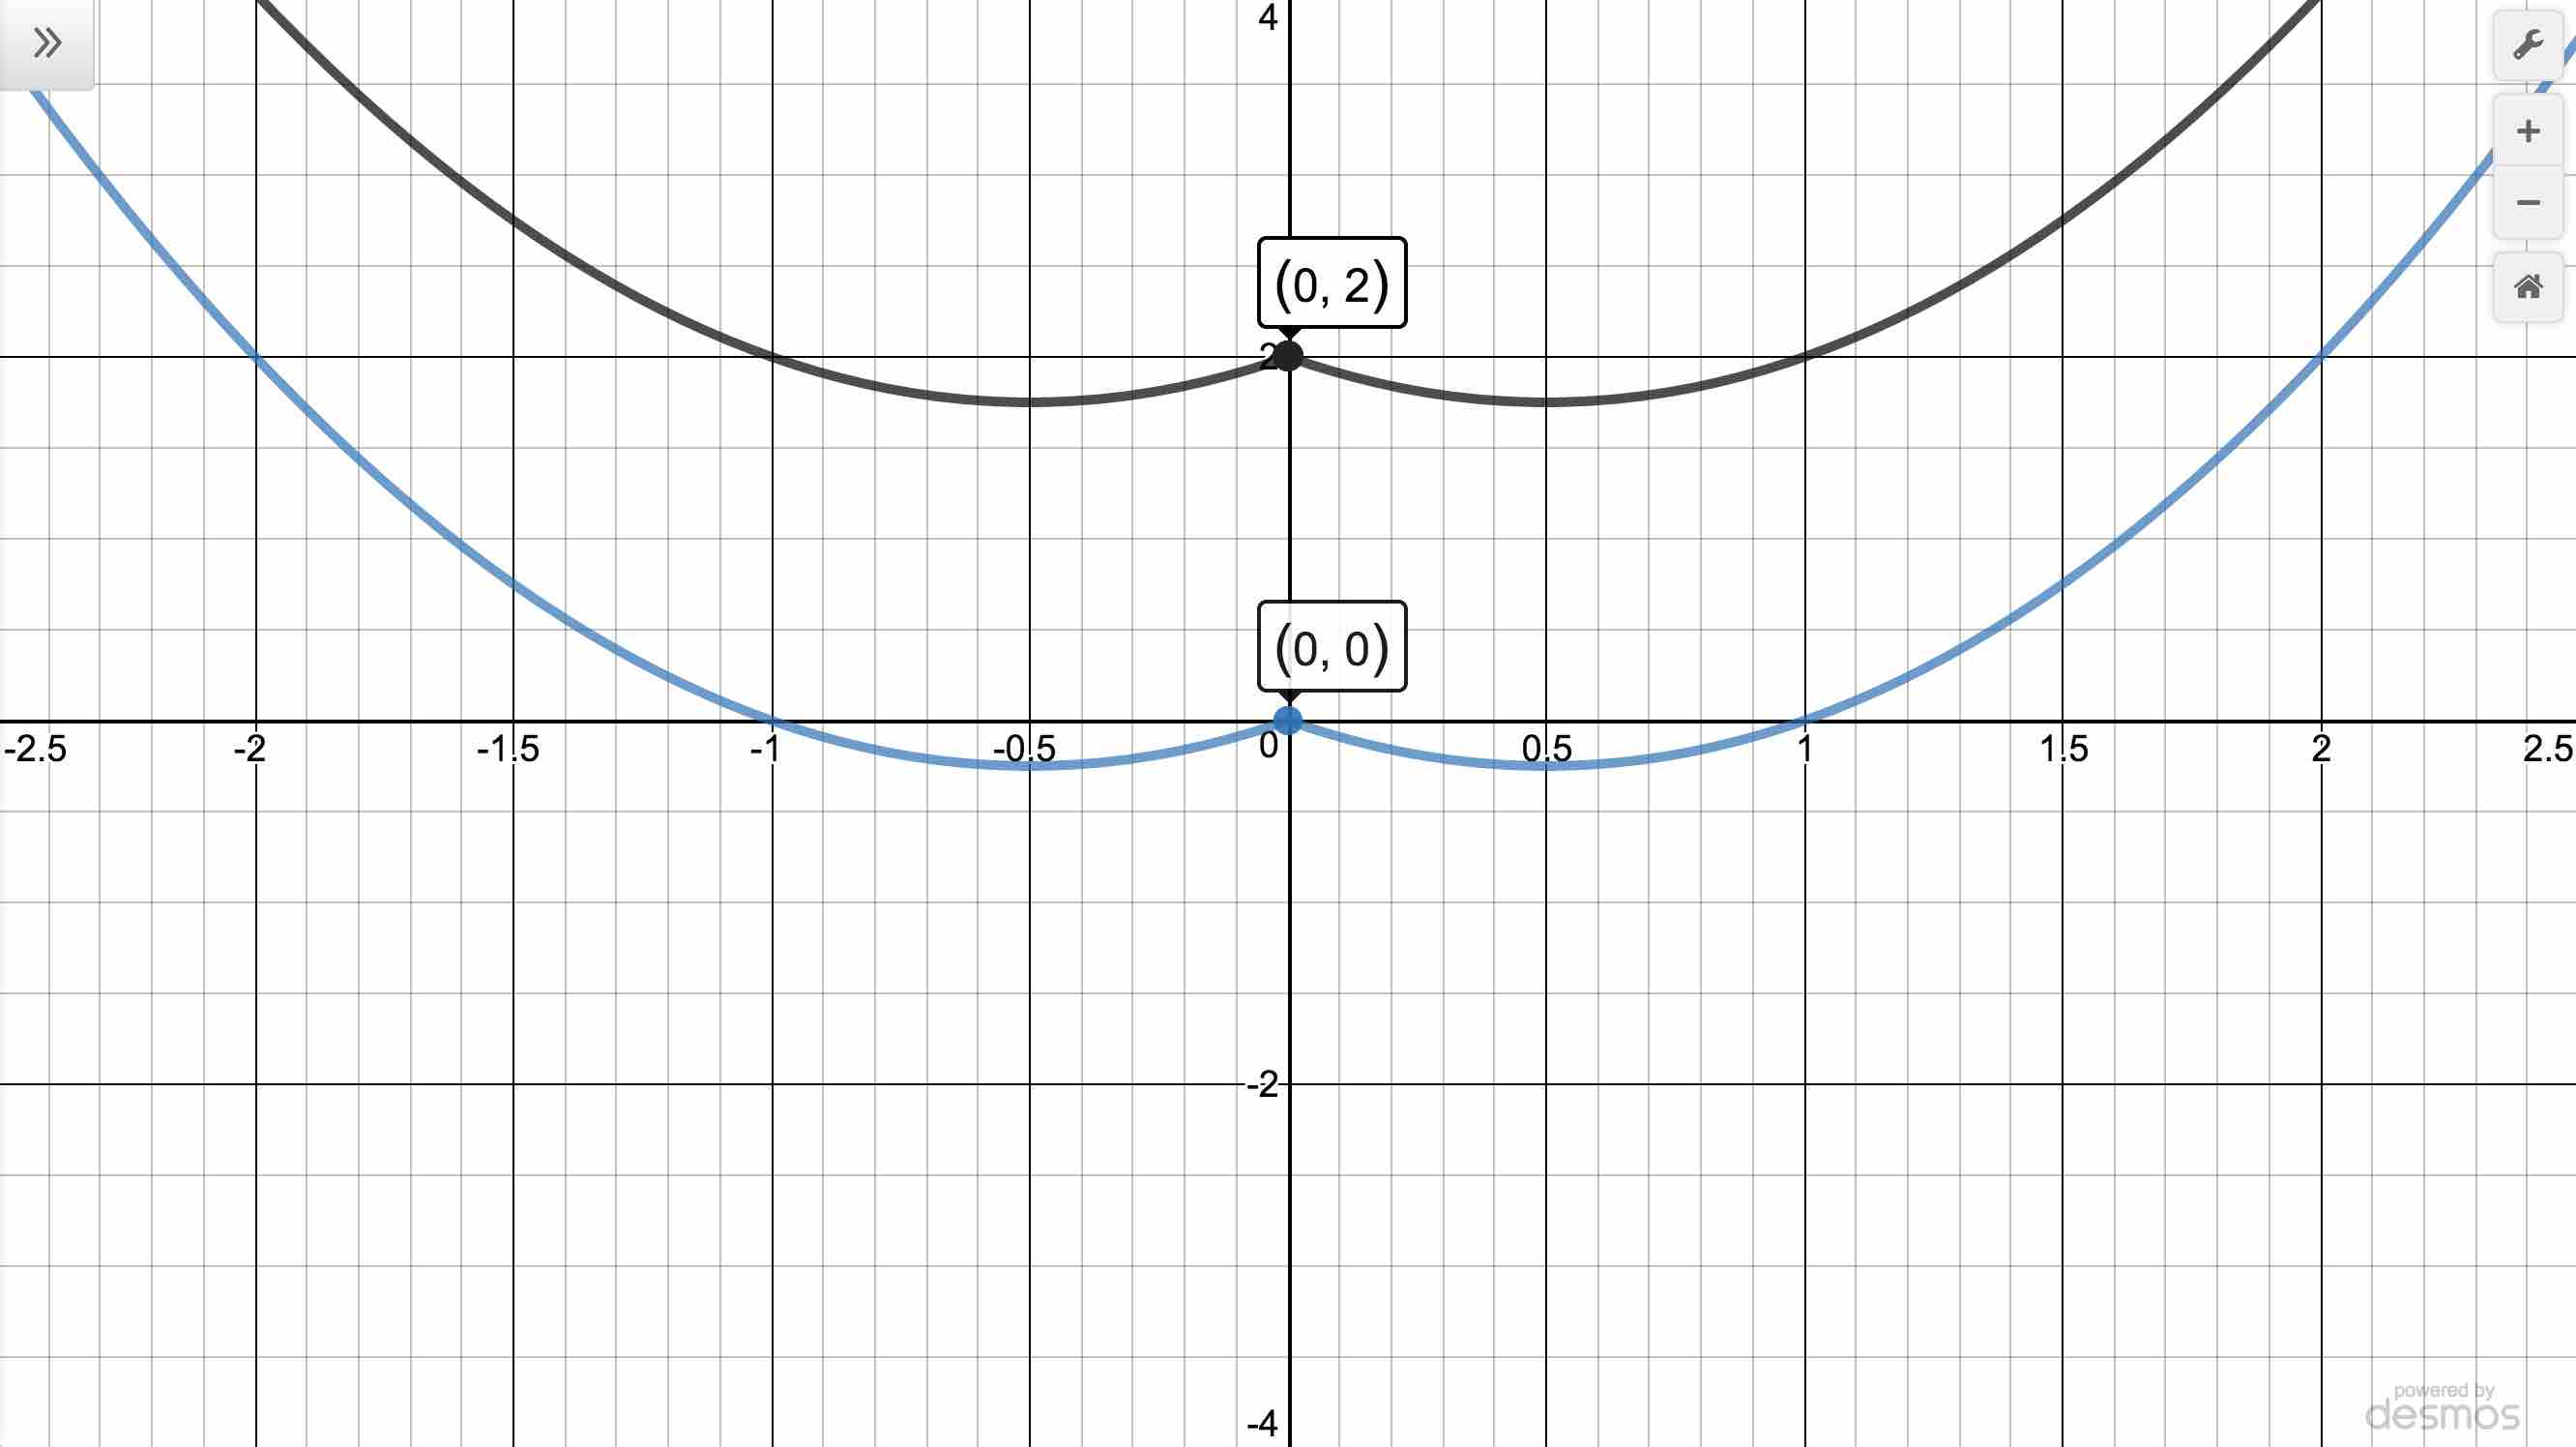
\includegraphics[width=3in]{./TransformationsGraphics/TransformationsEx04a.jpg} & 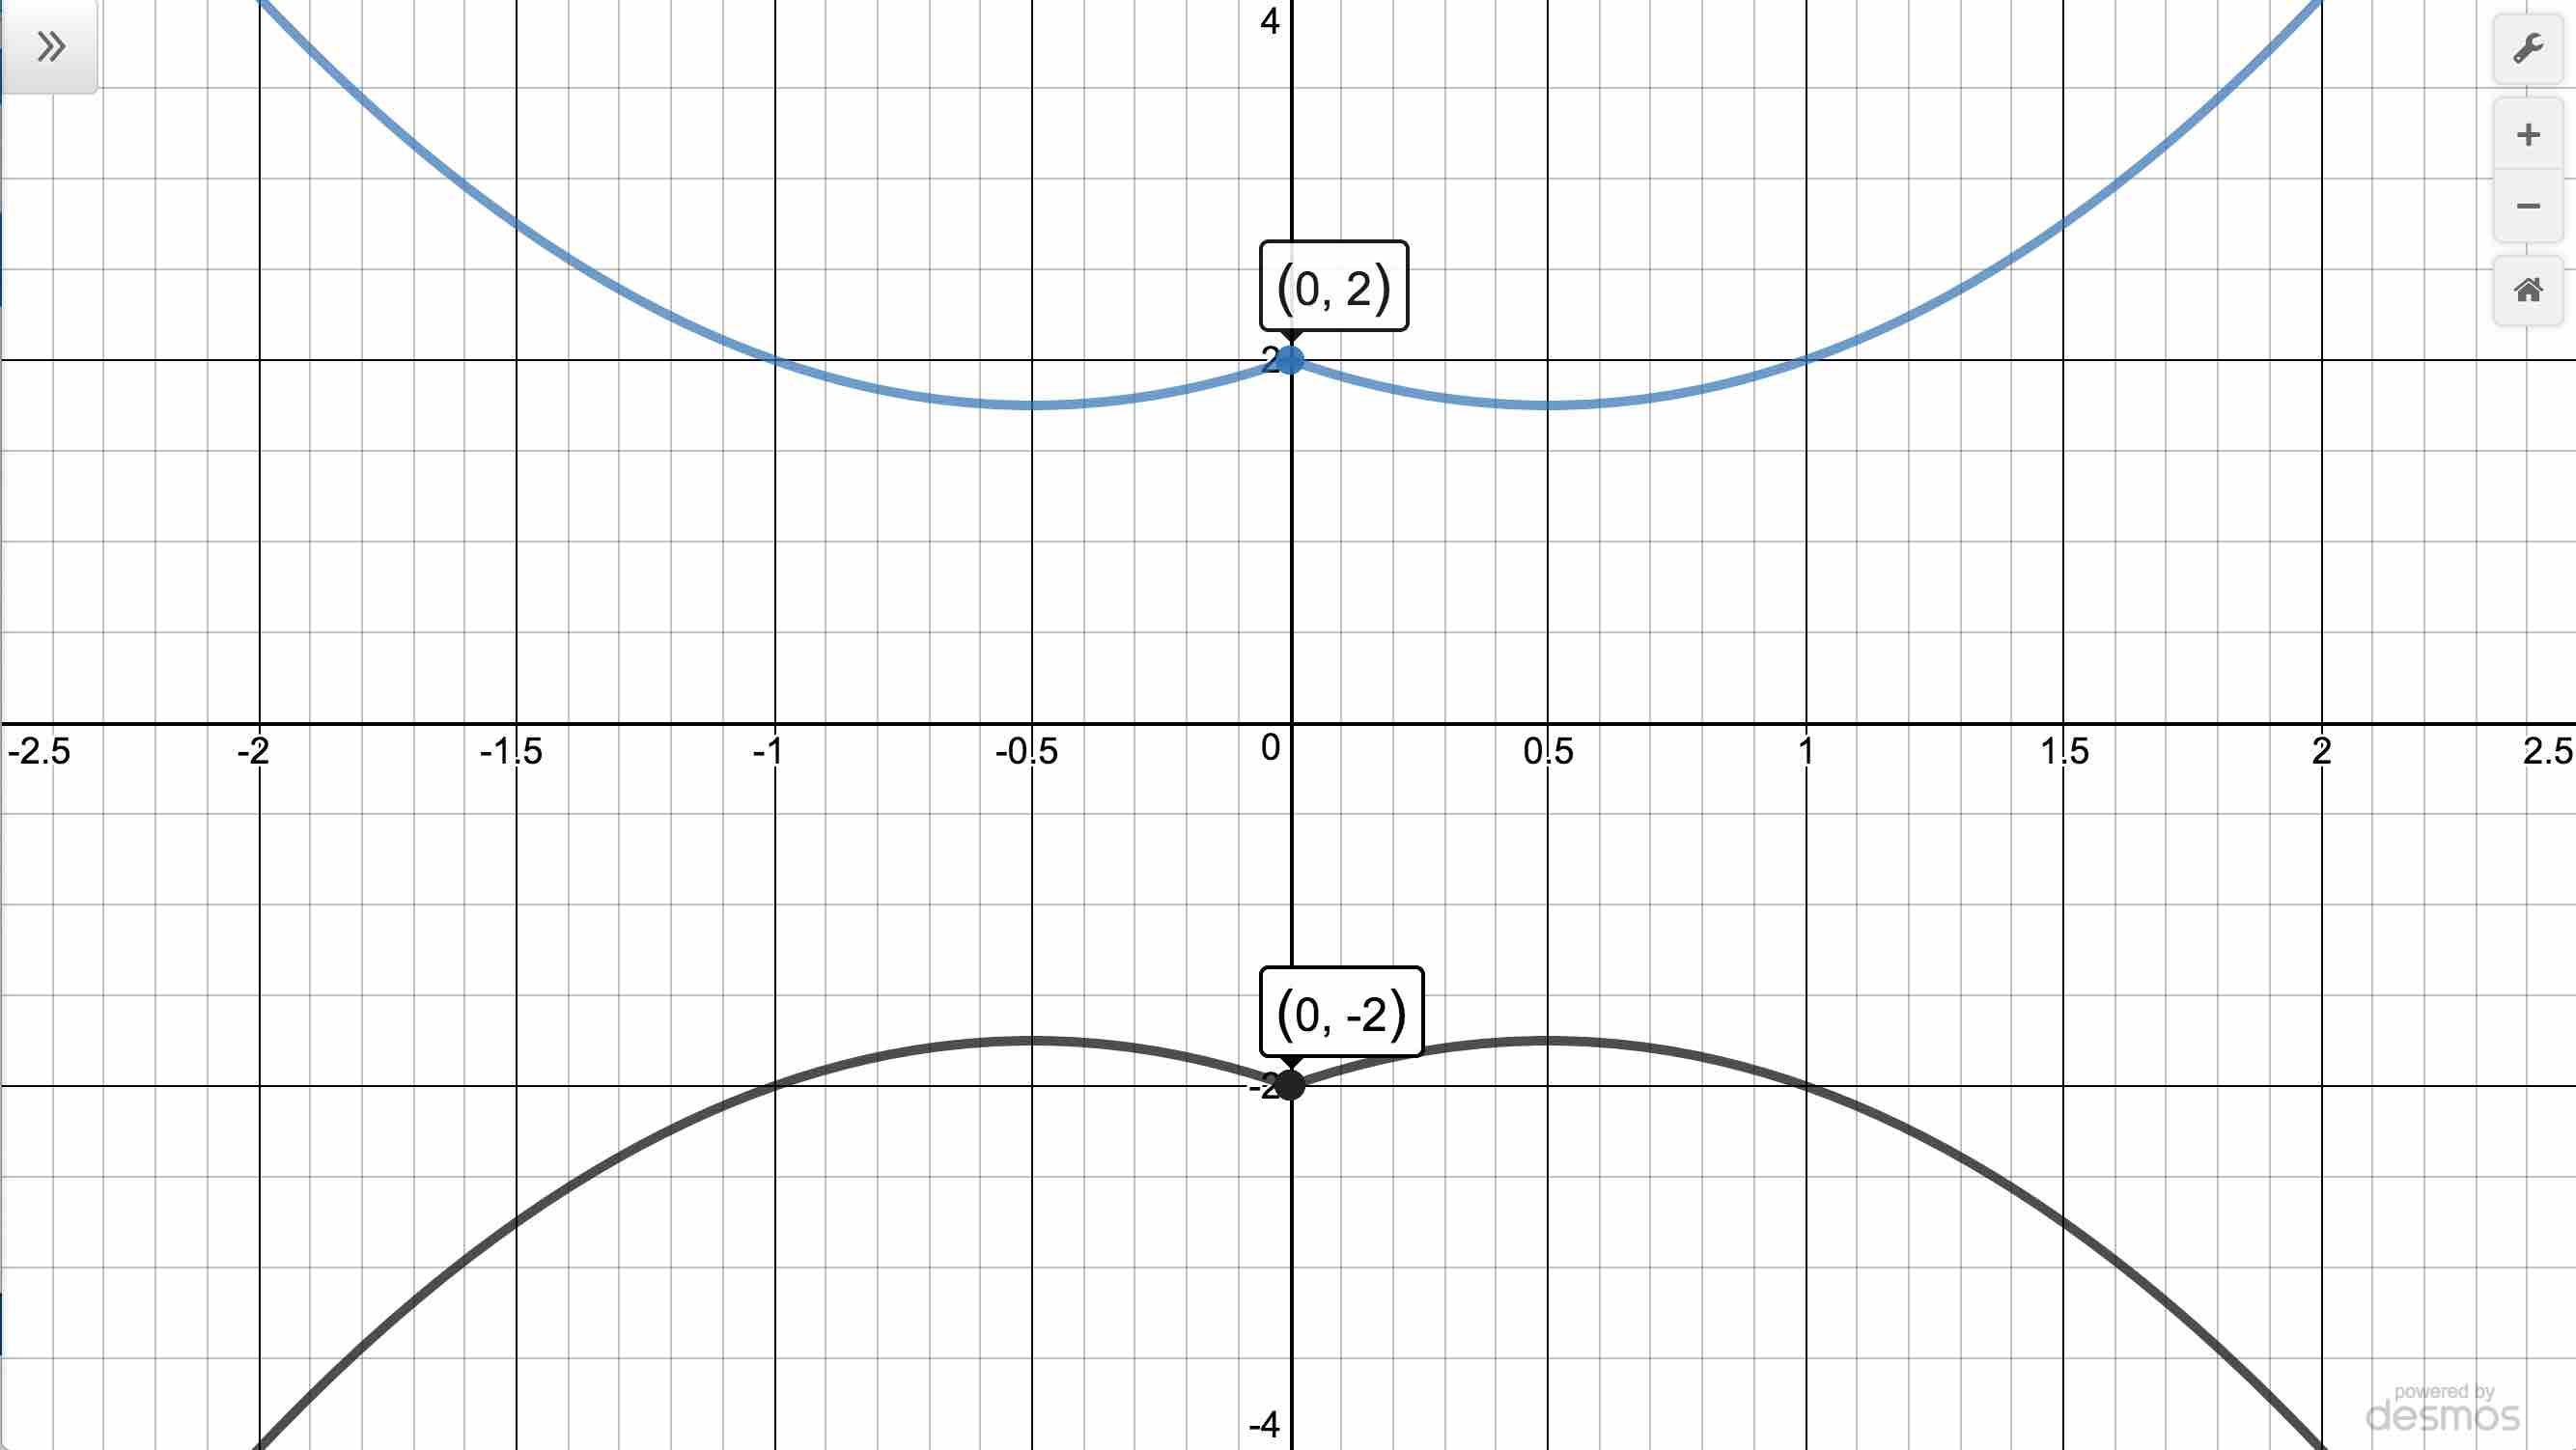
\includegraphics[width=3in]{./TransformationsGraphics/TransformationsEx04b.jpg} \\

$y=f(x)$ (lighter color) and $y=g_{1}(x) = f(x)+2$ &  $y = g_{1}(x)$ (lighter color) and $y = g_{2}(x) = -g_{1}(x)$ \\

\end{tabular}

\end{center} 

\item  Per Theorem \ref{hshifts}, $g_{3}(x) = g_{2}(x-1) = -(x-1)^2+|x-1|-2$.

\item  Per Theorem \ref{hscalings}, $g_{4}(x) = g_{3}(2x) = -(2x-1)^2+|2x-1| - 2$.

\begin{center}

\begin{tabular}{cc}

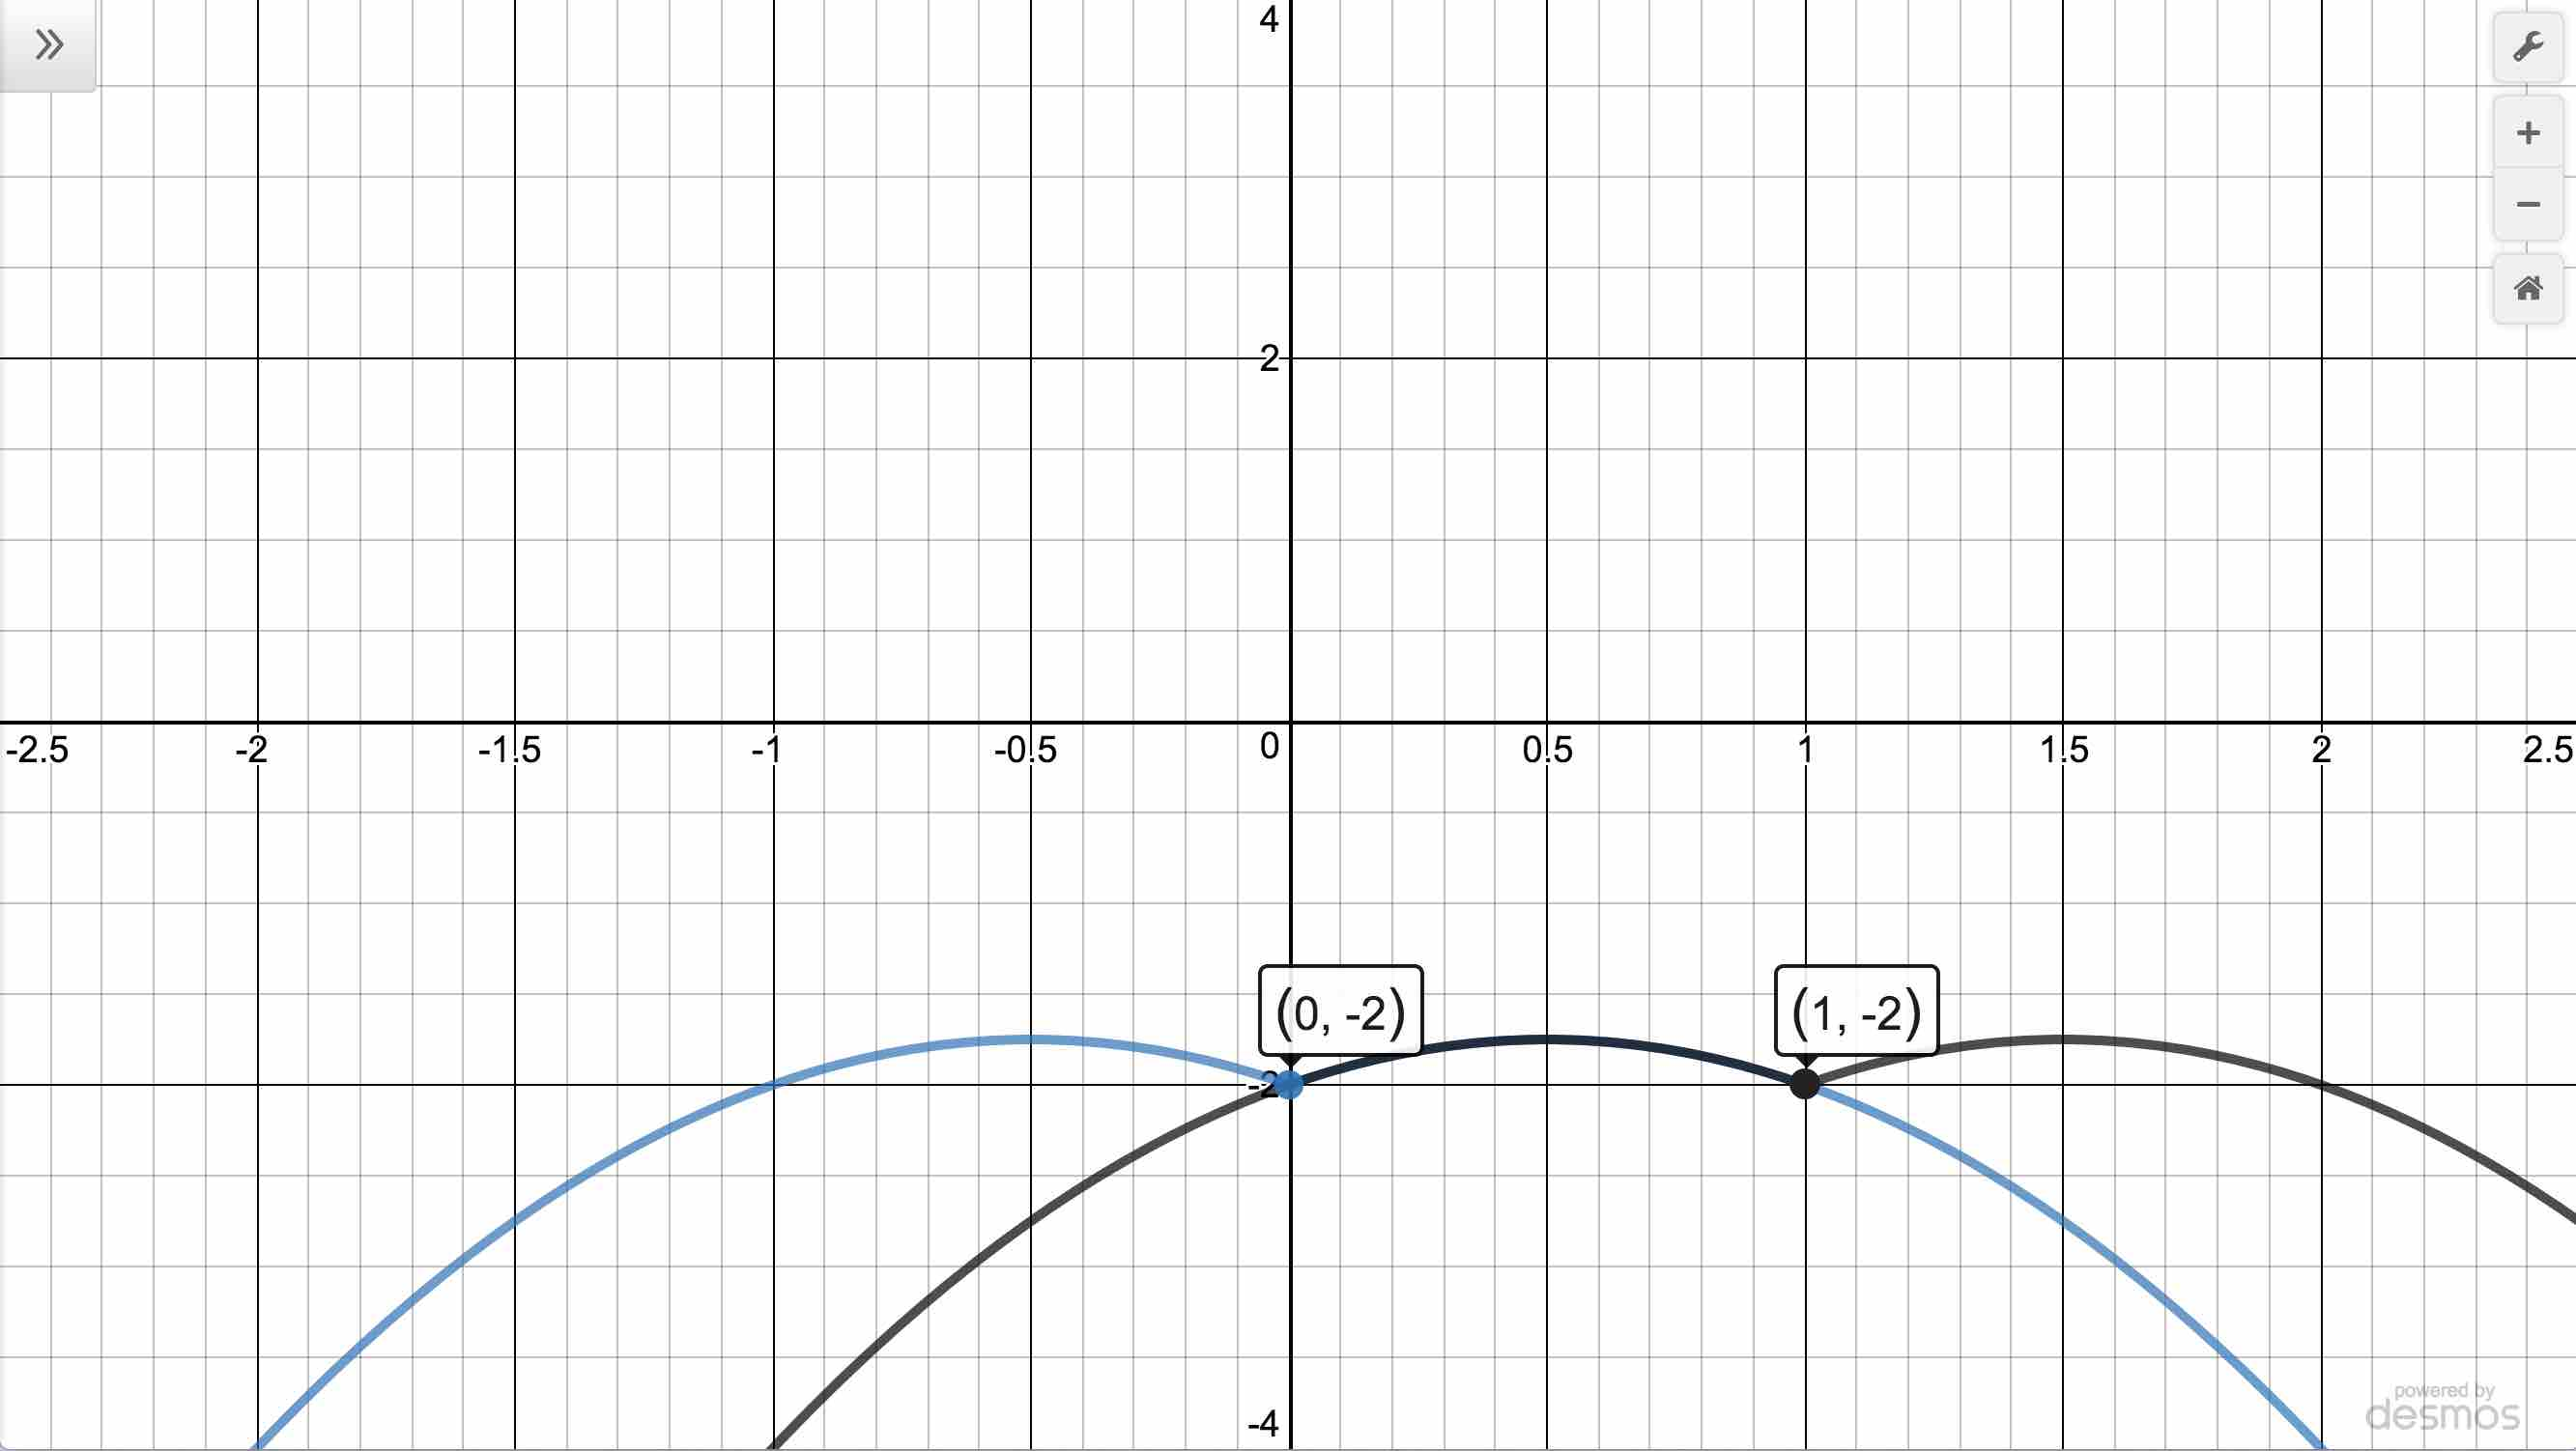
\includegraphics[width=3in]{./TransformationsGraphics/TransformationsEx04c.jpg} & 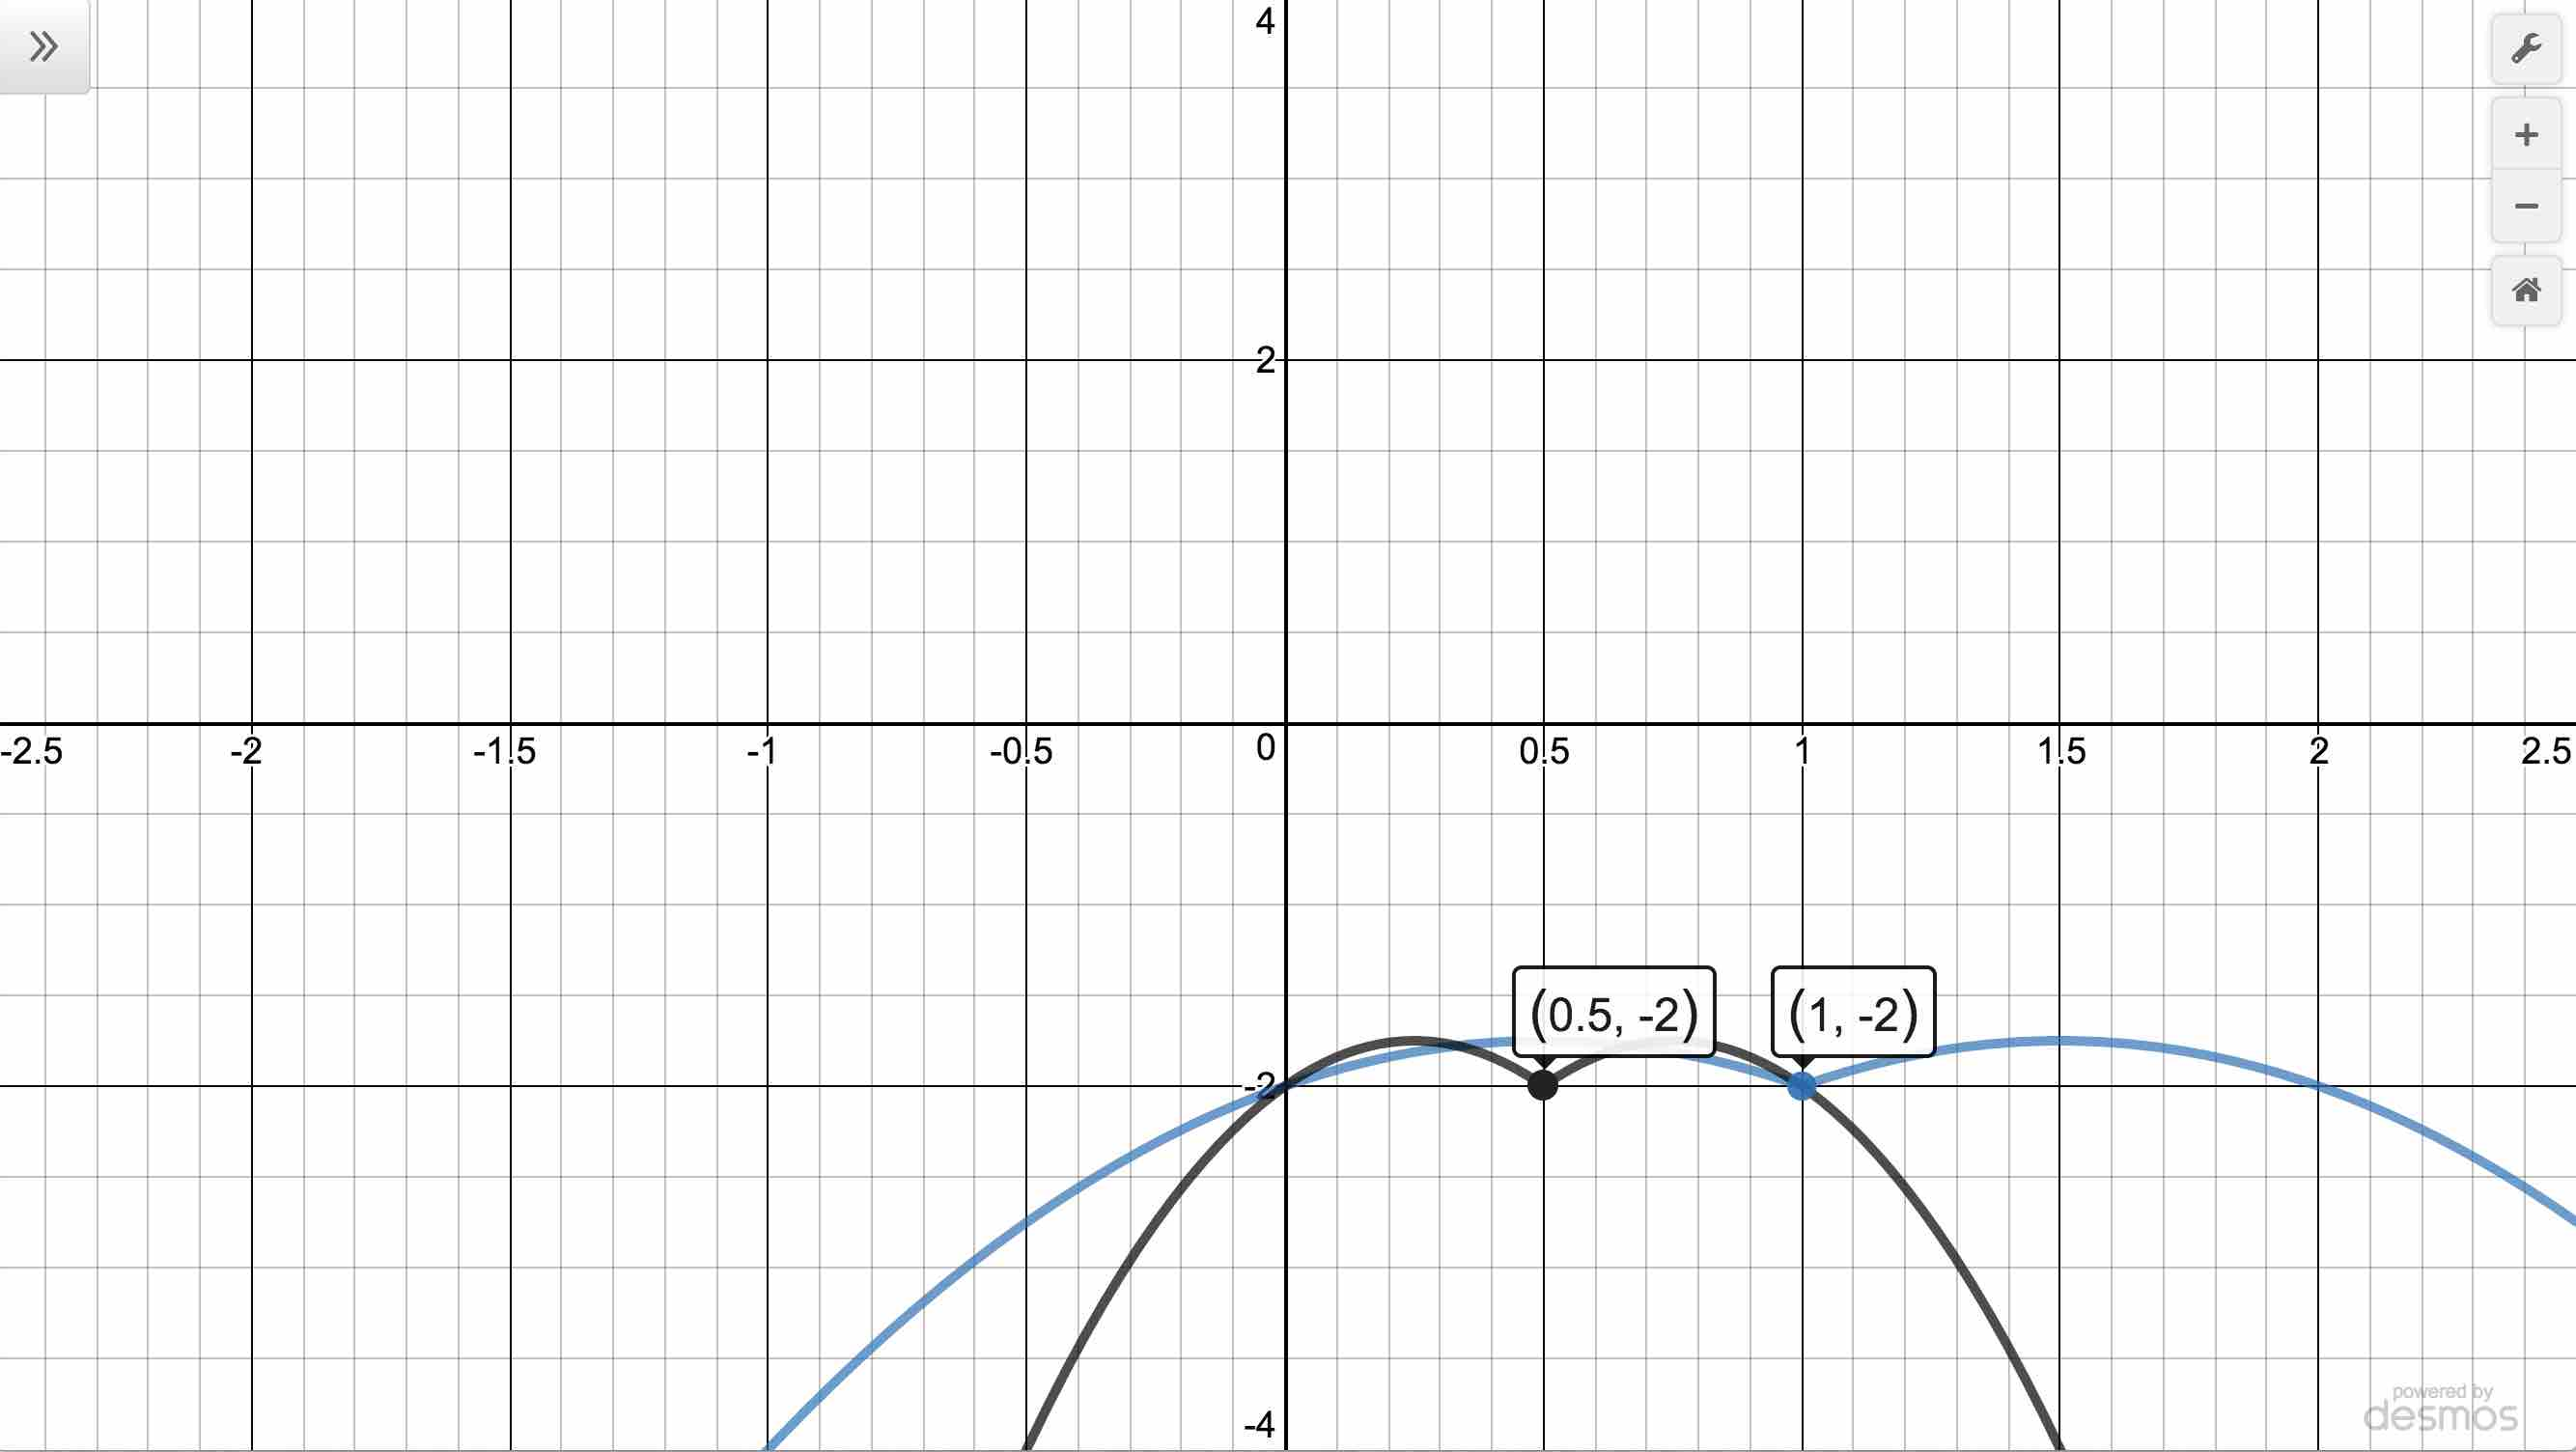
\includegraphics[width=3in]{./TransformationsGraphics/TransformationsEx04d.jpg} \\

$y=g_{2}(x)$ (lighter color) and $y=g_{3}(x) = g_{2}(x-1)$ &  $y = g_{3}(x)$ (lighter color) and $y = g_{4}(x) = g_{3}(2x)$ \\

\end{tabular}

\end{center} 

\item  Per Theorem \ref{vshifts}, $g_{5}(x) = g_{4}(x)+3 =  -(2x-1)^2+|2x-1| - 2 + 3 =  -(2x-1)^2+|2x-1| +1$.

\item  Per Theorem \ref{reflections}, $g_{6}(x) = g_{5}(-x)$:

\[ \begin{array}{rcl}

g_{6}(x) & = & g_{5}(-x) \\
 &  = &  -(2(-x)-1)^2+|2(-x)-1|+1 \\
  &  = & -(-2x-1)^2+|-2x-1|+1 \\
  &  = &  -[(-1)(2x+1)]^2+|[(-1)(2x+1)|+1 \\
  &  = &   -(-1)^2(2x+1)^2+|-1||2x+1| + 1 \\
  & =  & -(2x+1)^2+|2x+1|+1 \\
  
  \end{array} \]

\begin{center}

\begin{tabular}{cc}

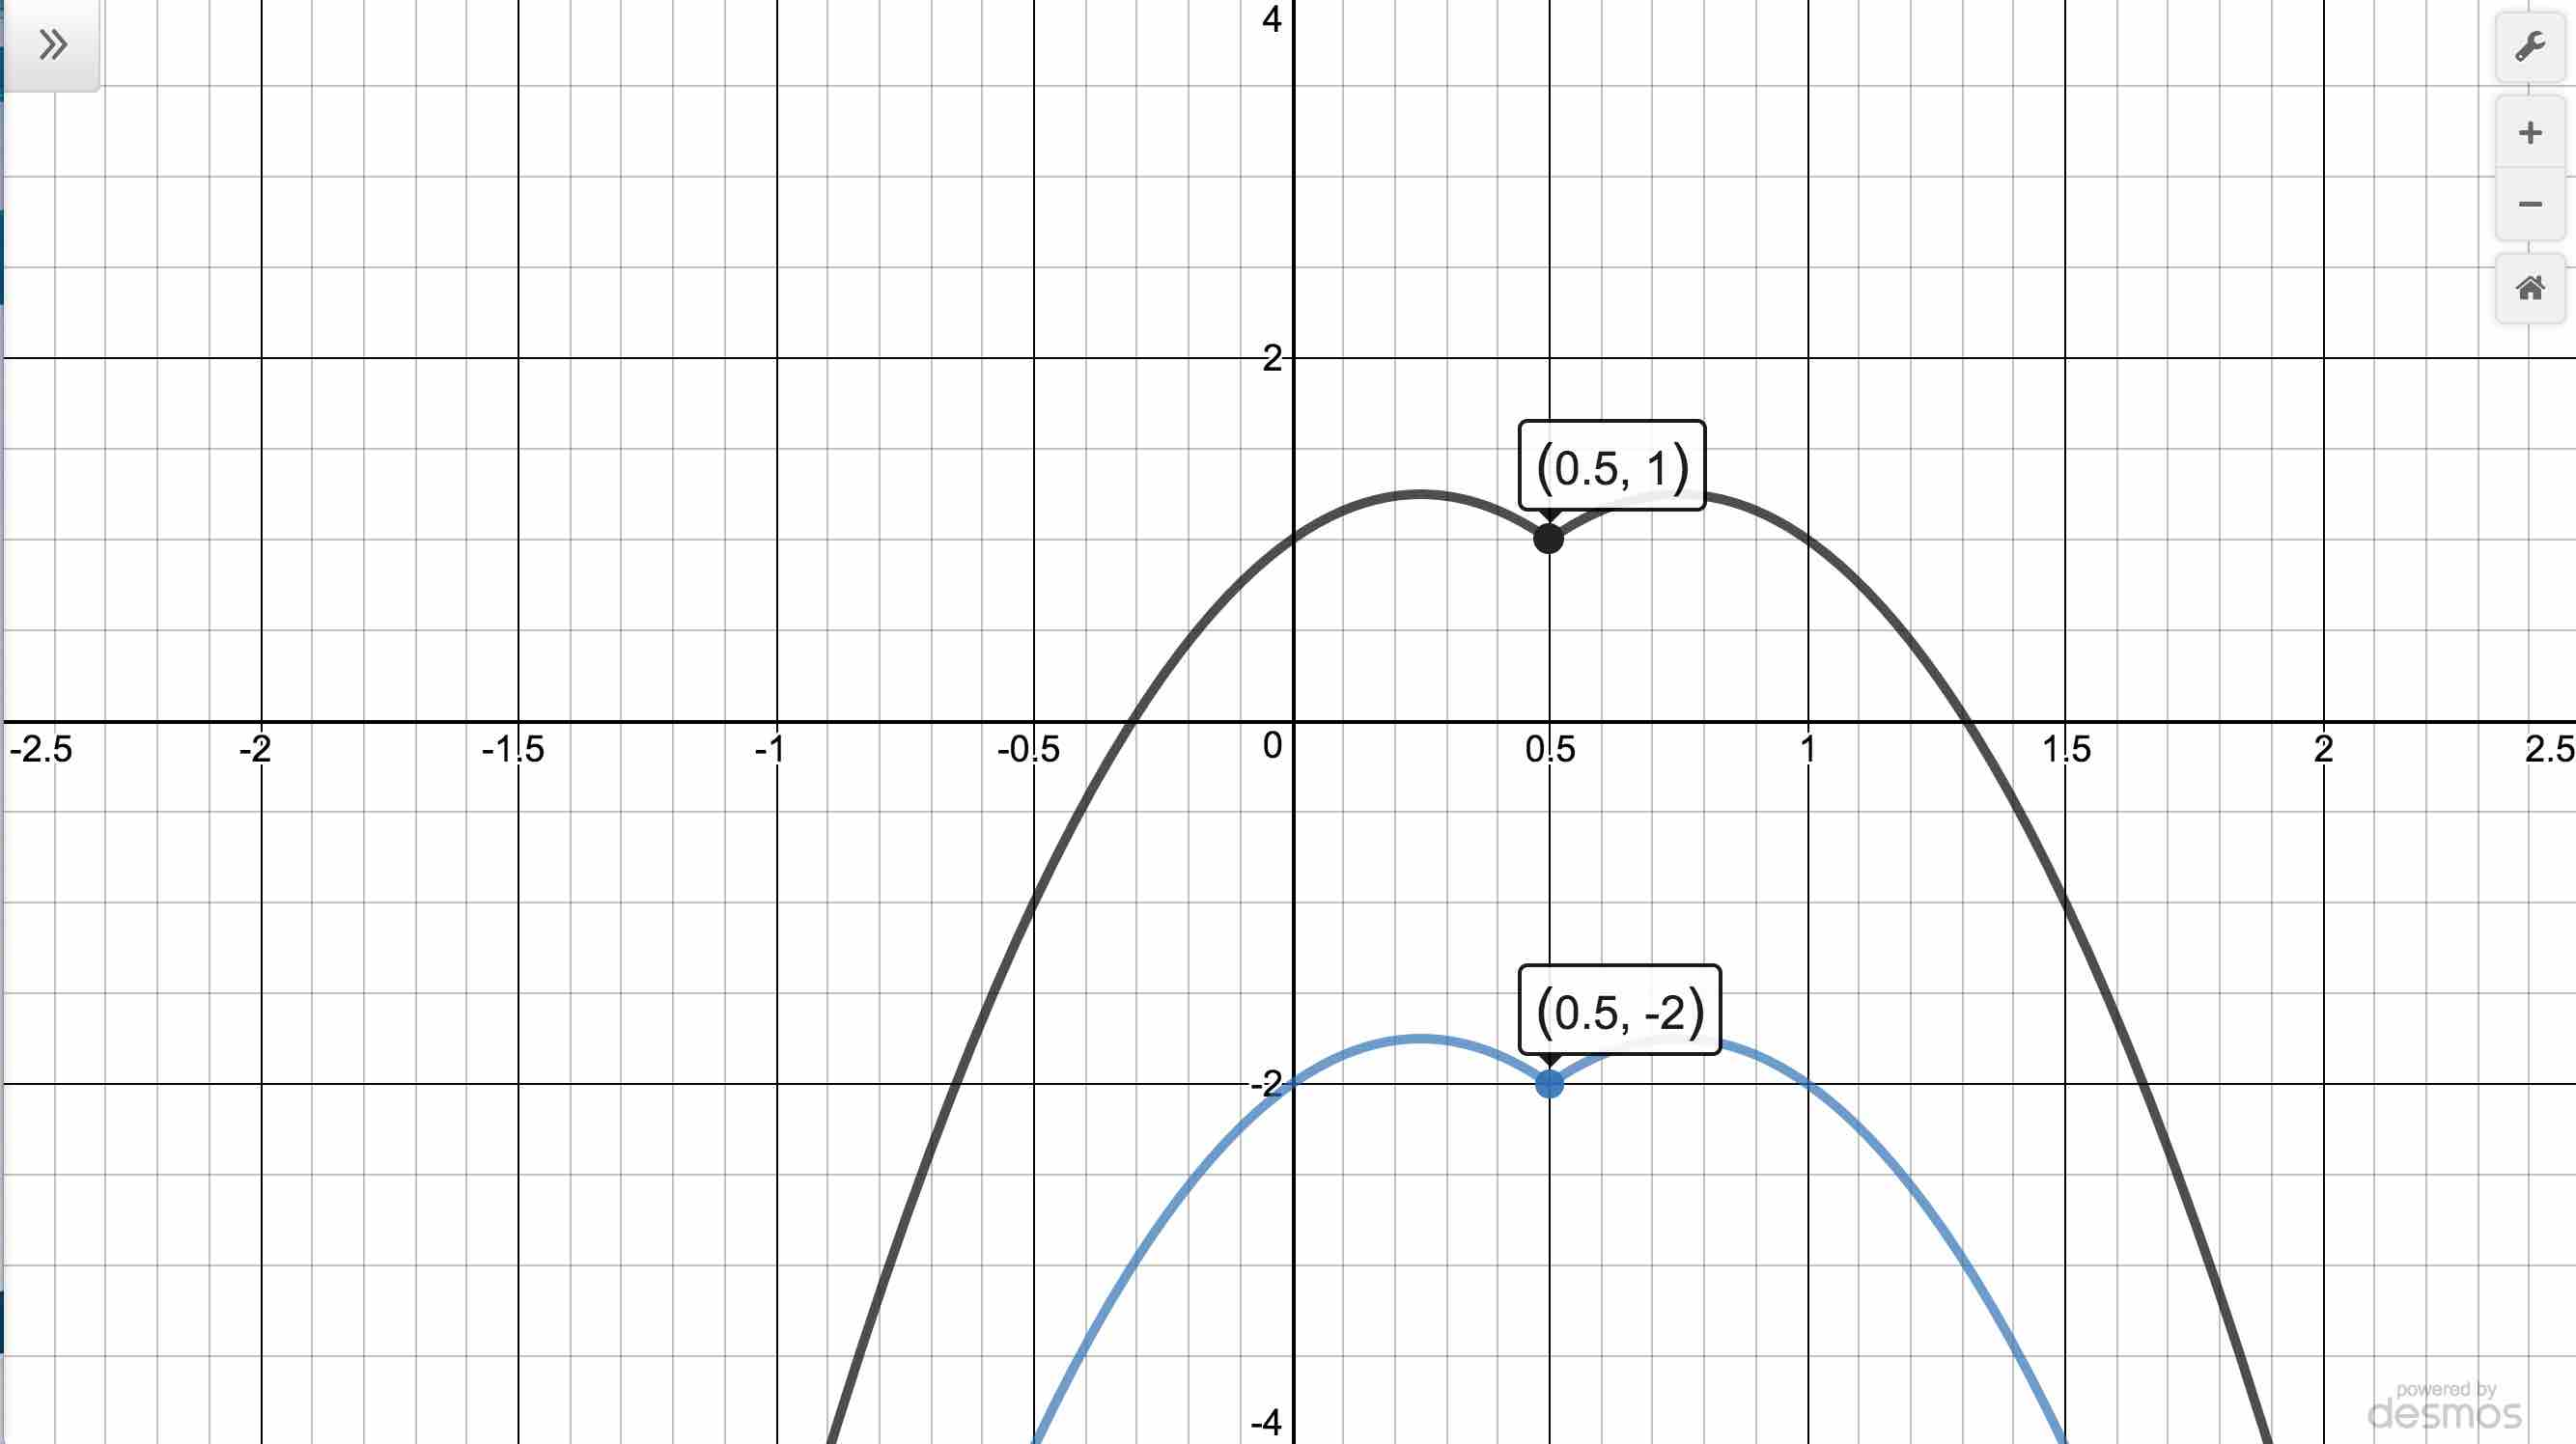
\includegraphics[width=3in]{./TransformationsGraphics/TransformationsEx04e.jpg} & 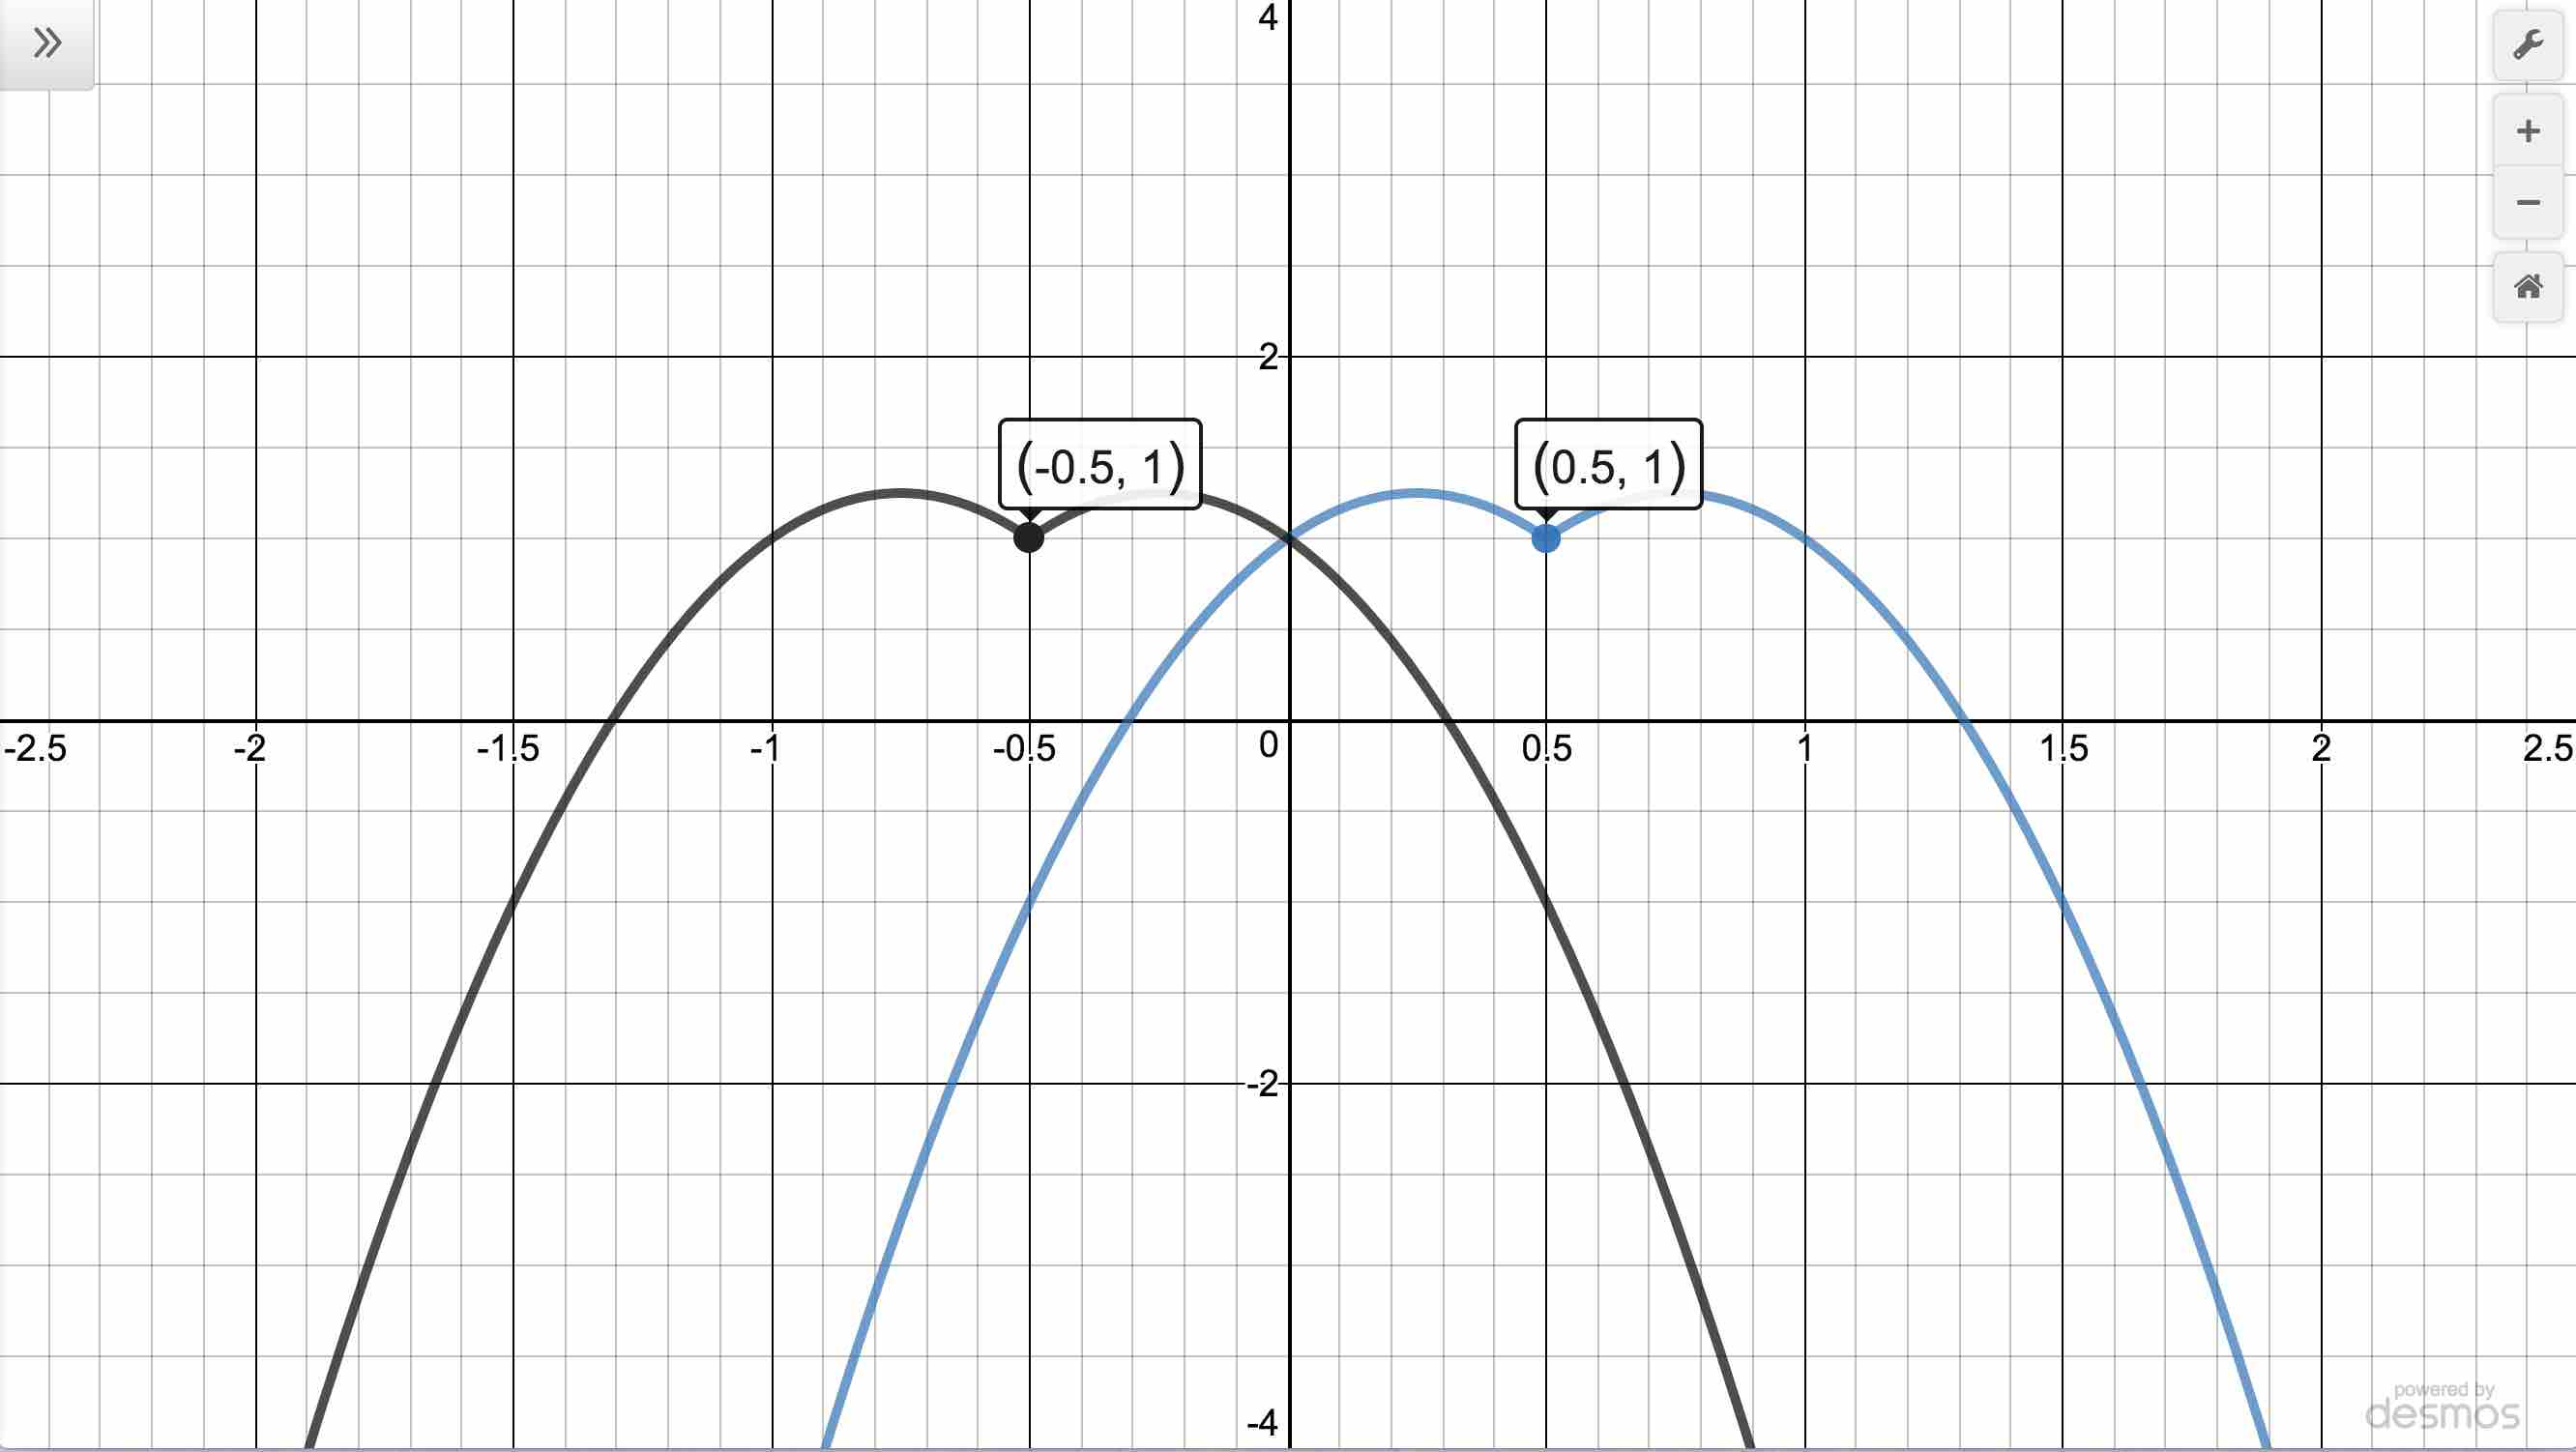
\includegraphics[width=3in]{./TransformationsGraphics/TransformationsEx04f.jpg} \\

$y=g_{4}(x)$ (lighter color) and $y=g_{5}(x) = g_{4}(x)+3$ &  $y = g_{5}(x)$ (lighter color) and $y = g_{6}(x) = g_{5}(-x)$ \\

\end{tabular}

\end{center} 

\end{enumerate}

Hence, $g(x) = g_{6}(x) = -(2x+1)^2+|2x+1| + 1$.  \qed
 
\end{ex}

It is instructive to show that the expression $g(x)$ in Example \ref{transsequenceex}  can be written as $g(x) = a f(bx-h)+k$.  

\smallskip

One way is to compare the graphs of $f$ and $g$ and work backwards.  A more methodical way is to repeat the work of Example \ref{transsequenceex}, but never substitute the formula for $f(x)$ as follows:


\begin{enumerate}

\item  Per Theorem \ref{vshifts}, $g_{1}(x) = f(x) + 2$.

\item  Per Theorem \ref{reflections}, $g_{2}(x) = -g_{1}(x) =  -[f(x) + 2] = -f(x)-2$.

\item  Per Theorem \ref{hshifts}, $g_{3}(x) = g_{2}(x-1) = -f(x-1)-2$.

\item  Per Theorem \ref{hscalings}, $g_{4}(x) = g_{3}(2x) =-f(2x-1)-2$.

\item  Per Theorem \ref{vshifts}, $g_{5}(x) = g_{4}(x)+3 = -f(2x-1)-2 + 3 = -f(2x-1)+1$.

\item  Per Theorem \ref{reflections}, $g_{6}(x) = g_{5}(-x) =  -f(2(-x)-1)+1 = -f(-2x-1)+1$.

\end{enumerate}

Hence $g(x) =  -f(-2x-1)+1$.  Note we can show $f$ is even,\footnote{Recall this means $f(-x) = f(x)$.} so $f(-2x-1) = f(-(2x+1)) = f(2x+1)$ and obtain $g(x) = -f(2x+1)+1$.  


At the beginning of this section, we discussed how all of the transformations we'd be discussing are the result of composing given functions with linear functions.  Not all transformations, not even all rigid transformations,\footnote{See Section \ref{PolarGraphs}.} fall into these categories.  

\smallskip

For example, consider the graphs of $y=f(x)$ and $y=g(x)$ below.

\[ \begin{array}{ccc}
\phantomsection
\label{relatedbyabsgraphs}
\begin{mfpic}[14]{-1}{6}{-6}{6}
\tlabel[cc](1,-5){\scriptsize $(0,-5)$}
\tlabel[cc](1,0.5){\scriptsize $(2,0)$}
\tlabel[cc](3,3){\scriptsize $(4,3)$}
\tlabel[cc](6,3){\scriptsize $(5,3)$}
\tlabel[cc](6,-0.5){\scriptsize $x$}
\tlabel[cc](0.5,6){\scriptsize $y$}
\tcaption{\scriptsize $y=f(x)$}
\axes
\xmarks{1,2,3,4,5}
\ymarks{-1,-2,-3,-4,-5,1,2,3,4,5}
\tlpointsep{4pt}
\axislabels {x}{{\scriptsize $1$} 1,  {\scriptsize $3$} 3, {\scriptsize $4$} 4, {\scriptsize $5$} 5}
\axislabels {y}{{\scriptsize $-1$} -1,{\scriptsize $-2$} -2, {\scriptsize $-3$} -3, {\scriptsize $-4$} -4,  {\scriptsize $1$} 1,{\scriptsize $2$} 2, {\scriptsize $3$} 3, {\scriptsize $4$} 4, {\scriptsize $5$} 5, {\scriptsize $-5$} -5}
\penwd{1.25pt}
\polyline{(0,-5), (2,0), (4,3), (5,3)}
\point[4pt]{(0,-5), (2,0), (4,3), (5,3)}
\end{mfpic}

&

\stackrel{\stackrel{}{\xrightarrow{\hspace{1in}}}}{\mbox{}} 

&


\begin{mfpic}[14]{-1}{6}{-6}{6}
\tlabel[cc](1,5){\scriptsize $(0,5)$}
\tlabel[cc](2,-0.5){\scriptsize $(2,0)$}
\tlabel[cc](3,3){\scriptsize $(4,3)$}
\tlabel[cc](6,3){\scriptsize $(5,3)$}
\tlabel[cc](6,-0.5){\scriptsize $x$}
\tlabel[cc](0.5,6){\scriptsize $y$}
\tcaption{\scriptsize $y=g(x)$}
\axes
\xmarks{1,2,3,4,5}
\ymarks{-1,-2,-3,-4,-5,1,2,3,4,5}
\tlpointsep{4pt}
\axislabels {x}{{\scriptsize $1$} 1,  {\scriptsize $3$} 3, {\scriptsize $4$} 4, {\scriptsize $5$} 5}
\axislabels {y}{{\scriptsize $-1$} -1,{\scriptsize $-2$} -2, {\scriptsize $1$} 1, {\scriptsize $-3$} -3, {\scriptsize $-4$} -4,  {\scriptsize $-5$} -5,{\scriptsize $2$} 2, {\scriptsize $3$} 3, {\scriptsize $4$} 4}
\penwd{1.25pt}
\polyline{(0,5), (2,0), (4,3), (5,3)}
\point[4pt]{(0,5), (2,0), (4,3), (5,3)}
\end{mfpic}

\end{array}\]




In Exercise \ref{relatedbyabsexercise}, we explore a non-linear transformation and revisit the pair of functions $f$ and $g$ then.



\newpage

\subsection{Exercises}

\label{ExercisesforTransformations}

Suppose $(2,-3)$ is on the graph of $y = f(x)$.  In Exercises \ref{transformpointfirst} - \ref{transformpointlast}, use Theorem \ref{transformationsthm} to find a point on the graph of the given transformed function.  

\begin{multicols}{3}
\begin{enumerate}

\item $y = f(x)+3$ \label{transformpointfirst}
\item $y = f(x+3)$
\item $y = f(x)-1$

\setcounter{HW}{\value{enumi}}
\end{enumerate}
\end{multicols}

\begin{multicols}{3}
\begin{enumerate}
\setcounter{enumi}{\value{HW}}

\item $y = f(x-1)$
\item $y = 3f(x)$
\item $y = f(3x)$

\setcounter{HW}{\value{enumi}}
\end{enumerate}
\end{multicols}

\begin{multicols}{3}
\begin{enumerate}
\setcounter{enumi}{\value{HW}}

\item $y = -f(x)$
\item $y = f(-x)$
\item $y = f(x-3)+1$

\setcounter{HW}{\value{enumi}}
\end{enumerate}
\end{multicols}

\begin{multicols}{3}
\begin{enumerate}
\setcounter{enumi}{\value{HW}}

\item $y = 2f(x+1)$
\item $y = 10 - f(x)$
\item $y = 3f(2x) - 1$

\setcounter{HW}{\value{enumi}}
\end{enumerate}
\end{multicols}

\begin{multicols}{3}
\begin{enumerate}
\setcounter{enumi}{\value{HW}}

\item $y = \frac{1}{2} f(4-x)$
\item $y = 5f(2x+1) + 3$
\item $y = 2f(1-x) -1$

\setcounter{HW}{\value{enumi}}
\end{enumerate}
\end{multicols}

\begin{multicols}{3}
\begin{enumerate}
\setcounter{enumi}{\value{HW}}

\item $y =f\left(\dfrac{7-2x}{4}\right)$
\item $y = \dfrac{f(3x) - 1}{2}$
\item $y = \dfrac{4-f(3x-1)}{7}$ \label{transformpointlast}

\setcounter{HW}{\value{enumi}}
\end{enumerate}
\end{multicols}



The complete graph of $y = f(x)$ is given below.  In Exercises \ref{transformgraphfirst} - \ref{transformgraphlast}, use it and Theorem \ref{transformationsthm} to graph the given transformed function.

\vspace{-.1in}
\begin{center}

\begin{mfpic}[15]{-5}{5}{-1}{5}
\axes
\tlabel[cc](5,-0.25){\scriptsize $x$}
\tlabel[cc](0.25,5){\scriptsize $y$}
\tlabel[cc](-2.5,1.25){\scriptsize $(-2,2)$}
\tlabel[cc](0.75,-0.5){\scriptsize $(0,0)$}
\tlabel[cc](2.25,1.25){\scriptsize $(2,2)$}
\tcaption{The graph of $y = f(x)$ for Ex. \ref{transformgraphfirst} - \ref{transformgraphlast}}
\xmarks{-4,-3,-2,-1,2,3,4}
\ymarks{1,2,3,4}
\tlpointsep{5pt}
\scriptsize
\axislabels {x}{{$-4 \hspace{7pt}$} -4,{$-3 \hspace{7pt}$} -3, {$-2 \hspace{7pt}$} -2, {$-1 \hspace{7pt}$} -1, {$2$} 2,{$3$} 3,{$4$} 4}
\axislabels {y}{{$1$} 1, {$2$} 2, {$3$} 3, {$4$} 4}
\normalsize
\penwd{1.25pt}
\arrow \reverse \arrow \polyline{(-4,4), (0,0), (4,4)}
\point[4pt]{(-2,2), (0,0), (2,2)}
\end{mfpic} 

\end{center}

\begin{multicols}{3}
\begin{enumerate}
\setcounter{enumi}{\value{HW}}

\item $y = f(x) + 1$ \label{transformgraphfirst}
\item $y = f(x) - 2$
\item $y = f(x+1)$

\setcounter{HW}{\value{enumi}}
\end{enumerate}
\end{multicols}

\begin{multicols}{3}
\begin{enumerate}
\setcounter{enumi}{\value{HW}}

\item $y = f(x - 2)$
\item $y = 2f(x)$
\item $y = f(2x)$

\setcounter{HW}{\value{enumi}}
\end{enumerate}
\end{multicols}

\begin{multicols}{3}
\begin{enumerate}
\setcounter{enumi}{\value{HW}}

\item $y = 2 - f(x)$
\item $y = f(2-x)$
\item $y = 2-f(2-x)$ \label{transformgraphlast}

\setcounter{HW}{\value{enumi}}
\end{enumerate}
\end{multicols}


\begin{enumerate}
\setcounter{enumi}{\value{HW}}

\item \label{somegraphsthesame} Some of the answers to Exercises \ref{transformgraphfirst} - \ref{transformgraphlast} above should be the same.  Which ones match up?  What properties of the graph of $y=f(x)$ contribute to the duplication?

\item  The function $f$ used in  Exercises \ref{transformgraphfirst} - \ref{transformgraphlast} should look familiar.  What is $f(x)$?  How does this this explain some of the duplication in the answers to Exercises \ref{transformgraphfirst} - \ref{transformgraphlast} mentioned in Exercise \ref{somegraphsthesame}?

\setcounter{HW}{\value{enumi}}
\end{enumerate}

\newpage

The complete graph of $y =g(t)$ is given below.  In Exercises \ref{transsecondgraphfirst} - \ref{transsecondgraphlast}, use it and Theorem \ref{transformationsthm} to graph the given transformed function.

\vspace{-.1in}
\begin{center}

\begin{mfpic}[15]{-5}{5}{-5}{5}
\axes
\tlabel[cc](5,-0.25){\scriptsize $t$}
\tlabel[cc](0.25,5){\scriptsize $y$}
\tlabel[cc](-2.25,-1.25){\scriptsize $(-2,0)$}
\tlabel[cc](1,4){\scriptsize $(0,4)$}
\tlabel[cc](2,-1.25){\scriptsize $(2,0)$}
\tlabel[cc](4,-2.5){\scriptsize $(4,-2)$}
\tcaption{The graph of $y = g(t)$ for Ex. \ref{transsecondgraphfirst} - \ref{transsecondgraphlast}}
\xmarks{-4,-3,-2,-1,1,2,3,4}
\ymarks{-4,-3,-2,-1,1,2,3,4}
\tlpointsep{5pt}
\scriptsize
\axislabels {x}{{$-4 \hspace{7pt}$} -4,{$-3 \hspace{7pt}$} -3, {$-1 \hspace{7pt}$} -1,{$1$} 1,{$3$} 3,{$4$} 4}
\axislabels {y}{{$-4$} -4,{$-3$} -3,{$-2$} -2, {$-1$} -1, {$1$} 1, {$2$} 2, {$3$} 3, {$4$} 4}
\normalsize
\penwd{1.25pt}
\polyline{(-2,0), (0,4), (2,0), (4,-2)}
\point[4pt]{(-2,0), (0,4), (2,0), (4,-2)}
\end{mfpic} 

\end{center}

\begin{multicols}{3}
\begin{enumerate}
\setcounter{enumi}{\value{HW}}

\item  $y = g(t) - 1$ \label{transsecondgraphfirst}
\item  $y = g(t + 1)$
\item  $y = \frac{1}{2} g(t)$

\setcounter{HW}{\value{enumi}}
\end{enumerate}
\end{multicols}

\begin{multicols}{3}
\begin{enumerate}
\setcounter{enumi}{\value{HW}}

\item  $y = g(2t)$
\item  $y = - g(t)$
\item  $y = g(-t)$

\setcounter{HW}{\value{enumi}}
\end{enumerate}
\end{multicols}

\begin{multicols}{3}
\begin{enumerate}
\setcounter{enumi}{\value{HW}}

\item  $y = g(t+1) - 1$
\item  $y = 1 - g(t)$
\item  $y = \frac{1}{2}g(t+1)-1$ \label{transsecondgraphlast}

\setcounter{HW}{\value{enumi}}
\end{enumerate}
\end{multicols}

The complete graph of $y = f(x)$ is given below.  In Exercises \ref{transthirdgraphfirst} - \ref{transthirdgraphlast}, use it and Theorem \ref{transformationsthm} to graph the given transformed function.

\vspace{-.1in}
\begin{center}

\begin{mfpic}[20]{-4}{4}{-1.5}{4}
\axes
\tlabel[cc](-3,-1){\small $\left(-3, 0 \right)$}
\tlabel[cc](0.8,3.3){\small $\left(0, 3 \right)$}
\tlabel[cc](3,-1){\small $\left(3, 0 \right)$}
\tlabel[cc](4,-0.5){\scriptsize $x$}
\tlabel[cc](0.5,4){\scriptsize $y$}
\tcaption{The graph of $y = f(x)$ for Ex. \ref{transthirdgraphfirst} - \ref{transthirdgraphlast}}
\xmarks{-3,-2,-1,1,2,3}
\ymarks{-1,1,2,3}
\tlpointsep{5pt}
\scriptsize
\axislabels {x}{{$-3 \hspace{7pt}$} -3, {$-2 \hspace{7pt}$} -2, {$-1 \hspace{7pt}$} -1, {$1$} 1, {$2$} 2, {$3$} 3}
\axislabels {y}{{$-1$} -1, {$1$} 1, {$2$} 2}
\normalsize
\penwd{1.25pt}
\point[4pt]{(-3,0),(0,3)}
\parafcn{0,3.14159,0.1}{(3*cos(t), 3*sin(t))}
\pointfillfalse
\point[4pt]{(3,0)}
\end{mfpic}

\end{center}

\begin{multicols}{3}
\begin{enumerate}
\setcounter{enumi}{\value{HW}}

\item $g(x) = f(x) + 3$ \label{transthirdgraphfirst}
\item $h(x) = f(x) - \frac{1}{2}$
\item $j(x) = f\left(x - \frac{2}{3}\right)$

\setcounter{HW}{\value{enumi}}
\end{enumerate}
\end{multicols}

\begin{multicols}{3}
\begin{enumerate}
\setcounter{enumi}{\value{HW}}

\item $a(x) = f(x + 4)$
\item $b(x) = f(x + 1) - 1$ 
\item $c(x) = \frac{3}{5}f(x)$


\setcounter{HW}{\value{enumi}}
\end{enumerate}
\end{multicols}

\begin{multicols}{3}
\begin{enumerate}
\setcounter{enumi}{\value{HW}}


\item $d(x) = -2f(x)$
\item $k(x) = f\left(\frac{2}{3}x\right)$
\item $m(x) = -\frac{1}{4}f(3x)$

\setcounter{HW}{\value{enumi}}
\end{enumerate}
\end{multicols}

\begin{multicols}{3}
\begin{enumerate}
\setcounter{enumi}{\value{HW}}

\item $n(x) = 4f(x - 3) - 6$
\item $p(x) = 4 + f(1 - 2x)$
\item $q(x) = -\frac{1}{2}f\left(\frac{x + 4}{2}\right) - 3$ \label{transthirdgraphlast}

\setcounter{HW}{\value{enumi}}
\end{enumerate}
\end{multicols}

\newpage

The complete graph of $y = S(t)$ is given below. 

\vspace{-.1in}
\begin{center}

\begin{mfpic}[20]{-3}{3}{-4}{4}
\axes
\tlabel[cc](3,-0.25){\scriptsize $t$}
\tlabel[cc](0.25,4){\scriptsize $y$}
\tlabel[cc](-2,0.5){\scriptsize $(-2,0)$}
\tlabel[cc](-1,-3.5){\scriptsize $(-1,-3)$}
\tlabel[cc](0.5,0.25){\scriptsize $(0,0)$}
\tlabel[cc](1,3.5){\scriptsize $(1,3)$}
\tlabel[cc](2,-0.5){\scriptsize $(2,0)$}
\tcaption{The graph of $y=S(t)$}
\xmarks{-2,-1,1,2}
\ymarks{-3,-2,-1,1,2,3}
\tlpointsep{5pt}
\scriptsize
\axislabels {x}{{$-2 \hspace{7pt}$} -2,{$-1 \hspace{7pt}$} -1,{$1$} 1}
\axislabels {y}{{$-3$} -3,{$-2$} -2, {$-1$} -1, {$1$} 1, {$2$} 2, {$3$} 3}
\normalsize
\penwd{1.25pt}
\function{-2,2,0.1}{3*sin(1.570796327*x)}
\point[4pt]{(-2,0), (-1,-3), (0,0), (1,3), (2,0)}
\end{mfpic} 

\end{center}

The purpose of Exercises \ref{transformsinegraphfirst} - \ref{transformsinegraphlast} is to build up to the graph  of $y = \frac{1}{2}S(-t+1) + 1$  one step at a time.

\begin{multicols}{2}
\begin{enumerate}
\setcounter{enumi}{\value{HW}}

\item $y = S_{\text{\tiny $1$}}(t) = S(t + 1)$ \label{transformsinegraphfirst}
\item  $y = S_{\text{\tiny $2$}}(t) =  S_{\text{\tiny $1$}}(-t) = S(-t + 1)$

\setcounter{HW}{\value{enumi}}
\end{enumerate}
\end{multicols}

\begin{multicols}{2}
\begin{enumerate}
\setcounter{enumi}{\value{HW}}

\item  $y = S_{\text{\tiny $3$}}(t) = \frac{1}{2}  S_{\text{\tiny $2$}}(t) =  \frac{1}{2}S(-t+1)$
\item  $y = S_{\text{\tiny $4$}}(t) = S_{\text{\tiny $3$}}(t) + 1 = \frac{1}{2}S(-t+1) + 1$ \label{transformsinegraphlast}

\setcounter{HW}{\value{enumi}}
\end{enumerate}
\end{multicols}

Let $f(x) = \sqrt{x}$.  Find a formula for a function $g$ whose graph is obtained from $f$ from the given sequence of transformations. 

\begin{enumerate}
\setcounter{enumi}{\value{HW}}


\item  (1) shift right 2 units; (2) shift down 3 units

\item  (1) shift down 3 units; (2) shift right 2 units

\item  (1) reflect across the $x$-axis; (2) shift up 1 unit

\item  (1) shift up 1 unit; (2) reflect across the $x$-axis

\item  (1) shift left 1 unit; (2) reflect across the $y$-axis; (3) shift up 2 units

\item  (1) reflect across the $y$-axis;  (2) shift left 1 unit;  (3) shift up 2 units

\item  (1) shift left 3 units; (2) vertical stretch by a factor of 2; (3) shift down 4 units

\item  (1) shift left 3 units; (2) shift down 4 units; (3) vertical stretch by a factor of 2

\item  (1) shift right 3 units; (2) horizontal shrink by a factor of 2; (3) shift up 1 unit

\item  (1) horizontal shrink by a factor of 2; (2) shift right 3 units; (3) shift up 1 unit


\setcounter{HW}{\value{enumi}}
\end{enumerate}


\newpage

For Exercises \ref{findformulatransformationfirst} - \ref{findformulatransformationlast},  use the given of  $y = f(x)$ to write each function in terms of $f(x)$.
\begin{center}

\begin{mfpic}[15]{-5}{5}{-5}{5}
\axes
\tlabel[cc](5,-0.25){\scriptsize $x$}
\tlabel[cc](0.25,5){\scriptsize $y$}
\tlabel[cc](-2,-1.5){\scriptsize $\left(-\frac{1}{2},-\frac{3}{2} \right)$}
\tlabel[cc](-0.75,0.5){\scriptsize $(0,0)$}
\tlabel[cc](1.75,1.5){\scriptsize $\left(\frac{1}{2},\frac{3}{2} \right)$}
\tlabel[cc](3, 3.5){\scriptsize asymptote $y=3$}
\tlabel[cc](-2.75,-3.5){\scriptsize asymptote $y=-3$}
\tcaption{The graph of $y = f(x)$  for Ex. \ref{findformulatransformationfirst} - \ref{findformulatransformationlast}.}
\xmarks{-4,-3,-2,-1,1,2,3,4}
\ymarks{-4,-3,-2,-1,1,2,3,4}
\tlpointsep{5pt}
\scriptsize
%\axislabels {x}{{$-4 \hspace{7pt}$} -4,{$-3 \hspace{7pt}$} -3, {$-1 \hspace{7pt}$} -1,{$1$} 1,{$3$} 3,{$4$} 4}
%\axislabels {y}{{$-4$} -4,{$-3$} -3,{$-2$} -2, {$-1$} -1, {$1$} 1, {$2$} 2, {$3$} 3, {$4$} 4}
\normalsize
\dashed \polyline {(-5,3), (5,3)}
\dashed \polyline {(-5,-3), (5,-3)}
\penwd{1.25pt}
\arrow \reverse \arrow \parafcn{-2.8,2.8,0.1}{( 0.5*(tan( 0.5236*t))   ,   t   )}
\point[4pt]{(0,0), (0.5,1.5), (-0.5,-1.5)}
\end{mfpic} 

\end{center}

%\enlargethispage{1in}

\begin{multicols}{2}
\begin{enumerate}
\setcounter{enumi}{\value{HW}}

\item  \label{findformulatransformationfirst} $y = g(x)$ %$g(x)=f(x)+1$

\begin{mfpic}[15]{-5}{5}{-5}{5}
\axes
\tlabel[cc](5,-0.25){\scriptsize $x$}
\tlabel[cc](0.25,5){\scriptsize $y$}
\tlabel[cc](-2,-0.5){\scriptsize $\left(-\frac{1}{2},-\frac{1}{2} \right)$}
\tlabel[cc](-0.75,1.5){\scriptsize $(0,1)$}
\tlabel[cc](1.75,2.5){\scriptsize $\left(\frac{1}{2},\frac{5}{2} \right)$}
\tlabel[cc](3, 4.5){\scriptsize asymptote $y=4$}
\tlabel[cc](-2.75,-2.5){\scriptsize asymptote $y=-2$}
\xmarks{-4,-3,-2,-1,1,2,3,4}
\ymarks{-4,-3,-2,-1,1,2,3,4}
\tlpointsep{5pt}
\scriptsize
%\axislabels {x}{{$-4 \hspace{7pt}$} -4,{$-3 \hspace{7pt}$} -3, {$-1 \hspace{7pt}$} -1,{$1$} 1,{$3$} 3,{$4$} 4}
%\axislabels {y}{{$-4$} -4,{$-3$} -3,{$-2$} -2, {$-1$} -1, {$1$} 1, {$2$} 2, {$3$} 3, {$4$} 4}
\normalsize
\dashed \polyline {(-5,4), (5,4)}
\dashed \polyline {(-5,-2), (5,-2)}
\penwd{1.25pt}
\arrow \reverse \arrow \parafcn{-2.8,2.8,0.1}{( 0.5*(tan( 0.5236*t))   ,   t +1  )}
\point[4pt]{(0,1), (0.5,2.5), (-0.5,-0.5)}
\end{mfpic} 


\item  $y = h(x)$ %$h(x) = f(x-2)$

\begin{mfpic}[15]{-3}{7}{-5}{5}
\axes
\tlabel[cc](7,-0.25){\scriptsize $x$}
\tlabel[cc](0.25,5){\scriptsize $y$}
\gclear \tlabelrect(0,-1.5){\scriptsize $\left(\frac{3}{2},-\frac{3}{2} \right)$}
\tlabel[cc](1.25,0.5){\scriptsize $(2,0)$}
\tlabel[cc](3.75,1.5){\scriptsize $\left(\frac{5}{2},\frac{3}{2} \right)$}
\tlabel[cc](3, 3.5){\scriptsize asymptote $y=3$}
\gclear \tlabelrect(-0.75,-3.5){\scriptsize asymptote $y=-3$}
\xmarks{-2,-1,1,2,3,4,5,6}
\ymarks{-3, 2,3,4}
\tlpointsep{5pt}
\scriptsize
%\axislabels {x}{{$-4 \hspace{7pt}$} -4,{$-3 \hspace{7pt}$} -3, {$-1 \hspace{7pt}$} -1,{$1$} 1,{$3$} 3,{$4$} 4}
%\axislabels {y}{{$-4$} -4,{$-3$} -3,{$-2$} -2, {$-1$} -1, {$1$} 1, {$2$} 2, {$3$} 3, {$4$} 4}
\normalsize
\dashed \polyline {(-3,3), (7,3)}
\dashed \polyline {(-3,-3), (7,-3)}
\penwd{1.25pt}
\arrow \reverse \arrow \parafcn{-2.8,2.8,0.1}{( 2+(0.5*(tan( 0.5236*t)))    ,   t   )}
\point[4pt]{(2,0), (2.5,1.5), (1.5,-1.5)}
\end{mfpic} 


\setcounter{HW}{\value{enumi}}
\end{enumerate}
\end{multicols}



\begin{multicols}{2}
\begin{enumerate}
\setcounter{enumi}{\value{HW}}

\item   $y = p(x)$  % $p(x) = f\left( \frac{x}{2} \right) -1$

\begin{mfpic}[15]{-5}{5}{-5}{5}
\axes
\tlabel[cc](5,-0.25){\scriptsize $x$}
\tlabel[cc](0.25,5){\scriptsize $y$}
\tlabel[cc](-2,-2.5){\scriptsize $\left(-1,-\frac{5}{2} \right)$}
\tlabel[cc](-1,-1){\scriptsize $(0,-1)$}
\tlabel[cc](1.75,0.5){\scriptsize $\left(1,\frac{1}{2} \right)$}
\tlabel[cc](3, 2.5){\scriptsize asymptote $y=2$}
\tlabel[cc](-2.75,-4.5){\scriptsize asymptote $y=-4$}
\xmarks{-4 step 0.5 until 4}
\ymarks{-4,-3,-2,-1,1,2,3,4}
\tlpointsep{5pt}
\scriptsize
%\axislabels {x}{{$-4 \hspace{7pt}$} -4,{$-3 \hspace{7pt}$} -3, {$-1 \hspace{7pt}$} -1,{$1$} 1,{$3$} 3,{$4$} 4}
%\axislabels {y}{{$-4$} -4,{$-3$} -3,{$-2$} -2, {$-1$} -1, {$1$} 1, {$2$} 2, {$3$} 3, {$4$} 4}
\normalsize
\dashed \polyline {(-5,2), (5,2)}
\dashed \polyline {(-5,-4), (5,-4)}
\penwd{1.25pt}
\arrow \reverse \arrow \parafcn{-2.8,2.8,0.1}{( 0.5*(tan( 0.5236*t))   ,   t -1  )}
\point[4pt]{(0,-1), (0.5,0.5), (-0.5,-2.5)}
\end{mfpic} 


\item  $y = q(x)$  % $q(x) = -2f(x) = 2f(-x)$


\begin{mfpic}[15]{-5}{5}{-5}{5}
\axes
\tlabel[cc](5,-0.25){\scriptsize $x$}
\tlabel[cc](0.25,5){\scriptsize $y$}
\tlabel[cc](-2,1.5){\scriptsize $\left(-\frac{1}{2},3 \right)$}
\tlabel[cc](0.75,0.5){\scriptsize $(0,0)$}
\tlabel[cc](1.75,-1.5){\scriptsize $\left(\frac{1}{2} -3 \right)$}
\tlabel[cc](3, 3.5){\scriptsize asymptote $y=6$}
\tlabel[cc](-2.75,-3.5){\scriptsize asymptote $y=-6$}
\xmarks{-4,-3,-2,-1,1,2,3,4}
\ymarks{-4 step 0.5 until 4}
\tlpointsep{5pt}
\scriptsize
%\axislabels {x}{{$-4 \hspace{7pt}$} -4,{$-3 \hspace{7pt}$} -3, {$-1 \hspace{7pt}$} -1,{$1$} 1,{$3$} 3,{$4$} 4}
%\axislabels {y}{{$-4$} -4,{$-3$} -3,{$-2$} -2, {$-1$} -1, {$1$} 1, {$2$} 2, {$3$} 3, {$4$} 4}
\normalsize
\dashed \polyline {(-5,3), (5,3)}
\dashed \polyline {(-5,-3), (5,-3)}
\penwd{1.25pt}
\arrow \reverse \arrow \parafcn{-2.8,2.8,0.1}{( 0.5*(tan( 0.5236*t))   ,  -1*t   )}
\point[4pt]{(0,0), (0.5,-1.5), (-0.5,1.5)}
\end{mfpic} 



\setcounter{HW}{\value{enumi}}
\end{enumerate}
\end{multicols}

\newpage

\begin{multicols}{2}
\begin{enumerate}
\setcounter{enumi}{\value{HW}}

\item  $y = r(x)$ % $r(x) = 2f(x+1)-3$

\begin{mfpic}[15]{-6}{4}{-5}{5}
\axes
\tlabel[cc](4,-0.25){\scriptsize $x$}
\tlabel[cc](0.25,5){\scriptsize $y$}
\tlabel[cc](-3,-3){\scriptsize $\left(-\frac{3}{2},-6 \right)$}
\tlabel[cc](-2.5,-1.5){\scriptsize $(-1,-3)$}
\tlabel[cc](-1.5,0.5){\scriptsize $\left(-\frac{1}{2},0\right)$}
\tlabel[cc](3, 2){\scriptsize asymptote $y=3$}
\tlabel[cc](-2.75,-5){\scriptsize asymptote $y=-9$}
\xmarks{-5,-3,-2,-1,1,2,3}
\ymarks{-4 step 0.5 until 4}
\tlpointsep{5pt}
\scriptsize
%\axislabels {x}{{$-4 \hspace{7pt}$} -4,{$-3 \hspace{7pt}$} -3, {$-1 \hspace{7pt}$} -1,{$1$} 1,{$3$} 3,{$4$} 4}
%\axislabels {y}{{$-4$} -4,{$-3$} -3,{$-2$} -2, {$-1$} -1, {$1$} 1, {$2$} 2, {$3$} 3, {$4$} 4}
\normalsize
\dashed \polyline {(-6,1.5), (4,1.5)}
\dashed \polyline {(-6,-4.5), (4,-4.5)}
\penwd{1.25pt}
\arrow \reverse \arrow \parafcn{-2.8,2.8,0.1}{( (0.5*(tan( 0.5236*t)))-1   ,   t -1.5 )}
\point[4pt]{(-1,-1.5), (-0.5,0), (-1.5,-3)}
\end{mfpic} 


\item \label{findformulatransformationlast} $y = s(x)$ % $s(x) = 2f(-x+1)-3 = -2f(x-1)+3$  


\begin{mfpic}[15]{-4}{6}{-5}{5}
\axes
\tlabel[cc](6,-0.25){\scriptsize $x$}
\tlabel[cc](0.25,5){\scriptsize $y$}
\tlabel[cc](3,-3){\scriptsize $\left(\frac{3}{2},-6 \right)$}
\tlabel[cc](2.5,-1.5){\scriptsize $(1,-3)$}
\tlabel[cc](1.5,0.5){\scriptsize $\left(\frac{1}{2},0\right)$}
\tlabel[cc](3, 2){\scriptsize asymptote $y=3$}
\tlabel[cc](-2.75,-5){\scriptsize asymptote $y=-9$}
\xmarks{-4,-3,-2,-1,1,2,3,4,5}
\ymarks{-4 step 0.5 until 4}
\tlpointsep{5pt}
\scriptsize
%\axislabels {x}{{$-4 \hspace{7pt}$} -4,{$-3 \hspace{7pt}$} -3, {$-1 \hspace{7pt}$} -1,{$1$} 1,{$3$} 3,{$4$} 4}
%\axislabels {y}{{$-4$} -4,{$-3$} -3,{$-2$} -2, {$-1$} -1, {$1$} 1, {$2$} 2, {$3$} 3, {$4$} 4}
\normalsize
\dashed \polyline {(6,1.5), (-4,1.5)}
\dashed \polyline {(6,-4.5), (-4,-4.5)}
\penwd{1.25pt}
\arrow \reverse \arrow \parafcn{-2.8,2.8,0.1}{( (-0.5*(tan( 0.5236*t)))+1   ,   t -1.5 )}
\point[4pt]{(1,-1.5), (0.5,0), (1.5,-3)}
\end{mfpic} 


\setcounter{HW}{\value{enumi}}
\end{enumerate}
\end{multicols}

\begin{enumerate}
\setcounter{enumi}{\value{HW}}

\item The graph of $y = f(x) = \sqrt[3]{x}$ is given below on the left and the graph of $y = g(x)$ is given on the right. Find a formula for $g$ based on transformations of the graph of $f$.  Check your answer by confirming that the points shown on the graph of $g$ satisfy the equation $y = g(x)$.

\[ \begin{array}{cc}

\begin{mfpic}[10]{-12}{9}{-6}{6}
\axes
\tlabel[cc](9,-0.5){\scriptsize $x$}
\tlabel[cc](0.5,6){\scriptsize $y$}
\tlabel[cc](-8,-3){\scriptsize $(-8,-2)$}
\gclear \tlabelrect(-1,-2){\scriptsize $(-1,-1)$ \vphantom{$\dfrac{3}{2}$}}
\tlabel[cc](-1.5,0.5){\scriptsize $(0,0)$}
\tlabel[cc](1,2){\scriptsize $(1,1)$}
\tlabel[cc](8, 3){\scriptsize $(8,2)$}
%\xmarks{-11 step 1 until 8}
%\ymarks{-5 step 1 until 5}
\tlpointsep{4pt}
%\axislabels {x}{{\tiny $-11 \hspace{6pt}$} -11, {\tiny $-10 \hspace{6pt}$} -10, {\tiny $-9 \hspace{6pt}$} -9, {\tiny $-8 \hspace{6pt}$} -8, {\tiny $-7 \hspace{6pt}$} -7, {\tiny $-6 \hspace{6pt}$} -6, {\tiny $-5 \hspace{6pt}$} -5, {\tiny $-4 \hspace{6pt}$} -4, {\tiny $-3 \hspace{6pt}$} -3, {\tiny $-2 \hspace{6pt}$} -2, {\tiny $-1 \hspace{6pt}$} -1, {\tiny $1$} 1, {\tiny $2$} 2, {\tiny $3$} 3, {\tiny $4$} 4, {\tiny $5$} 5, {\tiny $6$} 6, {\tiny $7$} 7, {\tiny $8$} 8}
%\axislabels {y}{{\tiny $-5$} -5, {\tiny $-4$} -4, {\tiny $-3$} -3, {\tiny $-2$} -2, {\tiny $-1$} -1, {\tiny $1$} 1, {\tiny $2$} 2, {\tiny $3$} 3, {\tiny $4$} 4, {\tiny $5$} 5}
\penwd{1.25pt}
\arrow \reverse \arrow \parafcn{-2.1,2.1,0.1}{(t**3,t)}
\point[4pt]{(0,0), (-1, -1), (1, 1), (-8, -2), (8, 2)}
\tcaption{\scriptsize $y = \sqrt[3]{x}$}
\end{mfpic}

&

\begin{mfpic}[10]{-12}{9}{-6}{6}
\axes
\tlabel[cc](9,-0.5){\scriptsize $x$}
\tlabel[cc](0.5,6){\scriptsize $y$}
\tlabel[cc](-11,4){\scriptsize $(-11,3)$}
\tlabel[cc](-4,2){\scriptsize $(-4,1)$}
\tlabel[cc](-5,-1){\scriptsize $(-3,-1)$}
\tlabel[cc](-2.5,-4){\scriptsize $(-2,-3)$}
\tlabel[cc](5,-4){\scriptsize $(5,-5)$}
%\xmarks{-11 step 1 until 8}
%\ymarks{-5 step 1 until 5}
\tlpointsep{4pt}
%\axislabels {x}{{\tiny $-11 \hspace{6pt}$} -11, {\tiny $-10 \hspace{6pt}$} -10, {\tiny $-9 \hspace{6pt}$} -9, {\tiny $-8 \hspace{6pt}$} -8, {\tiny $-7 \hspace{6pt}$} -7, {\tiny $-6 \hspace{6pt}$} -6, {\tiny $-5 \hspace{6pt}$} -5, {\tiny $-4 \hspace{6pt}$} -4, {\tiny $-3 \hspace{6pt}$} -3, {\tiny $-2 \hspace{6pt}$} -2, {\tiny $-1 \hspace{6pt}$} -1, {\tiny $1$} 1, {\tiny $2$} 2, {\tiny $3$} 3, {\tiny $4$} 4, {\tiny $5$} 5, {\tiny $6$} 6, {\tiny $7$} 7, {\tiny $8$} 8}
%\axislabels {y}{{\tiny $-5$} -5, {\tiny $-4$} -4, {\tiny $-3$} -3, {\tiny $-2$} -2, {\tiny $-1$} -1, {\tiny $1$} 1, {\tiny $2$} 2, {\tiny $3$} 3, {\tiny $4$} 4, {\tiny $5$} 5}
\penwd{1.25pt}
\arrow \reverse \arrow \parafcn{-2.1,2.1,0.1}{((t**3 - 3),((-2*t) - 1))}
\point[4pt]{(-11,3), (-4,1), (-3,-1), (-2,-3), (5,-5)}
\tcaption{\scriptsize $y = g(x)$}
\end{mfpic}

\end{array} \]

\item  \label{CompLinearisLinearExercise}  Show that the composition of two linear functions is  a linear function. Hence any (finite) sequence of transformations discussed in this section can be combined into the form given in Theorem \ref{transformationsthm}.

(HINT:  Let $f(x) = ax +b$ and $g(x) = cx + d$.  Find $(f \circ g)(x)$.)

\item For many common functions, the properties of Algebra make a horizontal scaling the same as a vertical scaling by (possibly) a different factor.  For example,  $\sqrt{9x} = 3\sqrt{x}$, so a horizontal compression of $y = \sqrt{x}$ by a factor of $9$ results in the same graph as a vertical stretch of $y = \sqrt{x}$ by a factor of $3$.  

With the help of your classmates, find the equivalent vertical scaling produced by the horizontal scalings $y = (2x)^{3}, \, y = |5x|, \, y = \sqrt[3]{27x} \, $ and $\, y = \left(\frac{1}{2} x\right)^{2}$.  

What about $y = (-2x)^{3}, \, y = |-5x|, \, y = \sqrt[3]{-27x}\, $ and $\, y = \left(-\frac{1}{2} x\right)^{2}$?

\newpage

\item   \label{SymmetryandReflectionsExercise}  Discuss the following questions with your classmates.

\begin{itemize}
\item If $f$ is even, what happens when you reflect the graph of $y = f(x)$ across the $y$-axis? 
\item If $f$ is odd, what happens when you reflect the graph of $y = f(x)$ across the $y$-axis? 
\item  If $f$ is even, what happens when you reflect the graph of $y = f(x)$ across the $x$-axis? 
\item  If $f$ is odd, what happens when you reflect the graph of $y = f(x)$ across the $x$-axis?  
\item How would you describe symmetry about the origin in terms of reflections?
\end{itemize}

\item  We mentioned earlier in the section that, in general, the order in which transformations are applied matters, yet in our first example with two transformations the order did not matter. (You could perform the shift to the left followed by the shift down or you could shift down and then left to achieve the same result.)  With the help of your classmates, determine the situations in which order does matter and those in which it does not.

\item \label{relatedbyabsexercise}  This Exercise is a follow-up to Exercise \ref{makeaveewithabsval} in Section \ref{AbsoluteValueFunctions}.

\begin{enumerate}

\item For each of the following functions, use a graphing utility to compare the graph of $y = f(x)$ with the graphs of $y = |f(x)|$ and $y = f(|x|)$. 

\begin{multicols}{3}

\begin{itemize}

\item $f(x) = 3-x$

\item $f(x) = x^2-x-6$

\item $f(x) = \sqrt{x+3} - 1$

\end{itemize}

\end{multicols}

\item  In general, how does the graph of $y = |f(x)|$ compare with that of $y = f(x)$?  What about the graph of $y = f(|x|)$ and $y = f(x)$?

\co{\item  Referring to the functions $f$ and $g$ graphed on page \pageref{relatedbyabsgraphs}, write $g$ in terms of $f$.}

\end{enumerate}

\setcounter{HW}{\value{enumi}}
\end{enumerate}

\newpage

\subsection{Answers}

\begin{multicols}{3}
\begin{enumerate}

\item $(2,0)$
\item $(-1,-3)$
\item $(2,-4)$

\setcounter{HW}{\value{enumi}}
\end{enumerate}
\end{multicols}

\begin{multicols}{3}
\begin{enumerate}
\setcounter{enumi}{\value{HW}}

\item $(3,-3)$
\item $(2,-9)$
\item $\left(\frac{2}{3}, -3\right)$

\setcounter{HW}{\value{enumi}}
\end{enumerate}
\end{multicols}

\begin{multicols}{3}
\begin{enumerate}
\setcounter{enumi}{\value{HW}}

\item $(2,3)$
\item $(-2,-3)$
\item $(5,-2)$

\setcounter{HW}{\value{enumi}}
\end{enumerate}
\end{multicols}

\begin{multicols}{3}
\begin{enumerate}
\setcounter{enumi}{\value{HW}}

\item $(1,-6)$
\item $(2,13)$
\item $y = (1,-10)$

\setcounter{HW}{\value{enumi}}
\end{enumerate}
\end{multicols}

\begin{multicols}{3}
\begin{enumerate}
\setcounter{enumi}{\value{HW}}

\item $\left(2, -\frac{3}{2}\right)$
\item $\left(\frac{1}{2}, -12 \right)$
\item $(-1,-7)$

\setcounter{HW}{\value{enumi}}
\end{enumerate}
\end{multicols}

\begin{multicols}{3}
\begin{enumerate}
\setcounter{enumi}{\value{HW}}

\item $\left(-\frac{1}{2}, -3\right)$
\item $\left(\frac{2}{3}, -2 \right)$
\item $(1,1)$

\setcounter{HW}{\value{enumi}}
\end{enumerate}
\end{multicols}

\begin{multicols}{2}
\begin{enumerate}
\setcounter{enumi}{\value{HW}}

\item $y = f(x) + 1$

\begin{mfpic}[15]{-5}{5}{-1}{5}
\axes
\tlabel[cc](5,-0.25){\scriptsize $x$}
\tlabel[cc](0.25,5){\scriptsize $y$}
\tlabel[cc](-2.5,2.25){\scriptsize $(-2,3)$}
\tlabel[cc](0.75,0.5){\scriptsize $(0,1)$}
\tlabel[cc](2.25,2.25){\scriptsize $(2,3)$}
\xmarks{-4,-3,-2,-1,1,2,3,4}
\ymarks{1,2,3,4}
\tlpointsep{5pt}
\scriptsize
\axislabels {x}{{$-4 \hspace{7pt}$} -4,{$-3 \hspace{7pt}$} -3, {$-2 \hspace{7pt}$} -2, {$-1 \hspace{7pt}$} -1, {$1$} 1, {$2$} 2,{$3$} 3,{$4$} 4}
\axislabels {y}{{$1$} 1, {$2$} 2, {$3$} 3, {$4$} 4}
\normalsize
\penwd{1.25pt}
\arrow \reverse \arrow \polyline{(-4,5), (0,1), (4,5)}
\point[4pt]{(-2,3), (0,1), (2,3)}
\end{mfpic} 

\vfill

\columnbreak

\item $y = f(x) - 2$

\begin{mfpic}[15]{-5}{5}{-3}{3}
\axes
\tlabel[cc](5,-0.25){\scriptsize $x$}
\tlabel[cc](0.25,3){\scriptsize $y$}
\tlabel[cc](-2.5,-0.75){\scriptsize $(-2,2)$}
\tlabel[cc](0.75,-2.5){\scriptsize $(0,-2)$}
\tlabel[cc](2.25,-0.75){\scriptsize $(2,2)$}
\xmarks{-4,-3,-2,-1,1,2,3,4}
\ymarks{-2,-1,1,2}
\tlpointsep{5pt}
\scriptsize
\axislabels {x}{{$-4 \hspace{7pt}$} -4, {$-1 \hspace{7pt}$} -1, {$1$} 1,{$4$} 4}
\axislabels {y}{{$-2$} -2, {$-1$} -1, {$1$} 1, {$2$} 2}
\normalsize
\penwd{1.25pt}
\arrow \reverse \arrow \polyline{(-4,2), (0,-2), (4,2)}
\point[4pt]{(-2,0), (0,-2), (2,0)}
\end{mfpic} 

\setcounter{HW}{\value{enumi}}
\end{enumerate}
\end{multicols}

\begin{multicols}{2}
\begin{enumerate}
\setcounter{enumi}{\value{HW}}

\item $y = f(x+1)$

\begin{mfpic}[15]{-6}{4}{-1}{5}
\axes
\tlabel[cc](4,-0.25){\scriptsize $x$}
\tlabel[cc](0.25,5){\scriptsize $y$}
\tlabel[cc](-3.5,1.25){\scriptsize $(-3,2)$}
\tlabel[cc](-1,-0.5){\scriptsize $(-1,0)$}
\tlabel[cc](1.25,1.25){\scriptsize $(1,2)$}
\xmarks{-5,-4,-3,-2,-1,1,2,3}
\ymarks{1,2,3,4}
\tlpointsep{5pt}
\scriptsize
\axislabels {x}{{$-5 \hspace{7pt}$} -5,{$-4 \hspace{7pt}$} -4,{$-3 \hspace{7pt}$} -3, {$1$} 1, {$2$} 2,{$3$} 3}
\axislabels {y}{{$1$} 1, {$2$} 2, {$3$} 3, {$4$} 4}
\normalsize
\penwd{1.25pt}
\arrow \reverse \arrow \polyline{(-5,4), (-1,0), (3,4)}
\point[4pt]{(-3,2), (-1,0), (1,2)}
\end{mfpic} 

\vfill

\columnbreak

\item $y = f(x - 2)$

\begin{mfpic}[15]{-3}{7}{-1}{5}
\axes
\tlabel[cc](7,-0.25){\scriptsize $x$}
\tlabel[cc](0.25,5){\scriptsize $y$}
\tlabel[cc](0.75,2){\scriptsize $(0,2)$}
\tlabel[cc](2,-0.5){\scriptsize $(2,0)$}
\tlabel[cc](3,2){\scriptsize $(4,2)$}
\xmarks{-2,-1,1,2,3,4,5,6}
\ymarks{1,2,3,4}
\tlpointsep{5pt}
\scriptsize
\axislabels {x}{{$-2 \hspace{7pt}$} -2, {$-1 \hspace{7pt}$} -1, {$3$} 3,{$4$} 4,{$5$} 5,{$6$} 6}
\axislabels {y}{{$1$} 1, {$2$} 2,  {$4$} 4}
\normalsize
\penwd{1.25pt}
\arrow \reverse \arrow \polyline{(-2,4), (2,0), (6,4)}
\point[4pt]{(0,2), (2,0), (4,2)}
\end{mfpic} 

\setcounter{HW}{\value{enumi}}
\end{enumerate}
\end{multicols}

\begin{multicols}{2}
\begin{enumerate}
\setcounter{enumi}{\value{HW}}


\item $y = 2f(x)$

\begin{mfpic}[15]{-5}{5}{-1}{5}
\axes
\tlabel[cc](5,-0.25){\scriptsize $x$}
\tlabel[cc](0.25,5){\scriptsize $y$}
\tlabel[cc](-2.75,3.5){\scriptsize $(-2,4)$}
\tlabel[cc](0.75,-0.5){\scriptsize $(0,0)$}
\tlabel[cc](2.5,3.5){\scriptsize $(2,4)$}
\xmarks{-4,-3,-2,-1,2,3,4}
\ymarks{1,2,3,4}
\tlpointsep{5pt}
\scriptsize
\axislabels {x}{{$-4 \hspace{7pt}$} -4,{$-3 \hspace{7pt}$} -3, {$-2 \hspace{7pt}$} -2, {$-1 \hspace{7pt}$} -1, {$2$} 2,{$3$} 3,{$4$} 4}
\axislabels {y}{{$1$} 1, {$2$} 2, {$3$} 3, {$4$} 4}
\normalsize
\penwd{1.25pt}
\arrow \reverse \arrow \polyline{(-2.5,5), (0,0), (2.5,5)}
\point[4pt]{(-2,4), (0,0), (2,4)}
\end{mfpic} 


\vfill

\columnbreak

\item $y = f(2x)$

\begin{mfpic}[15]{-5}{5}{-1}{5}
\axes
\penwd{1.25pt}
\arrow \reverse \arrow \polyline{(-2.5,5), (0,0), (2.5,5)}
\point[4pt]{(-1,2), (0,0), (1,2)}
\tlabel[cc](5,-0.25){\scriptsize $x$}
\tlabel[cc](0.25,5){\scriptsize $y$}
\tlabel[cc](-1.75,1.5){\scriptsize $(-1,2)$}
\tlabel[cc](0.75,-0.5){\scriptsize $(0,0)$}
\tlabel[cc](1.5,1.5){\scriptsize $(1,2)$}
\xmarks{-4,-3,-2,-1,2,3,4}
\ymarks{1,2,3,4}
\tlpointsep{5pt}
\scriptsize
\axislabels {x}{{$-4 \hspace{7pt}$} -4,{$-3 \hspace{7pt}$} -3, {$-2 \hspace{7pt}$} -2, {$-1 \hspace{7pt}$} -1, {$2$} 2,{$3$} 3,{$4$} 4}
\axislabels {y}{{$1$} 1, {$2$} 2, {$3$} 3, {$4$} 4}
\normalsize
\end{mfpic} 


\setcounter{HW}{\value{enumi}}
\end{enumerate}
\end{multicols}

\begin{multicols}{2}
\begin{enumerate}
\setcounter{enumi}{\value{HW}}

\item $y = 2 - f(x)$

\begin{mfpic}[15]{-5}{5}{-2}{3}
\axes
\tlabel[cc](5,-0.25){\scriptsize $x$}
\tlabel[cc](0.25,3){\scriptsize $y$}
\tlabel[cc](-1.25,-0.5){\scriptsize $(-2,0)$}
\tlabel[cc](0.75,2){\scriptsize $(0,2)$}
\tlabel[cc](1.5,-0.5){\scriptsize $(2,0)$}
\xmarks{-4,-3,-2,-1,2,3,4}
\ymarks{-1,1,2}
\tlpointsep{5pt}
\scriptsize
\axislabels {x}{{$-4 \hspace{7pt}$} -4,{$-3 \hspace{7pt}$} -3,  {$3$} 3,{$4$} 4}
\axislabels {y}{{$1$} 1, {$2$} 2}
\normalsize
\penwd{1.25pt}
\arrow \reverse \arrow \polyline{(-4,-2), (0,2), (4,-2)}
\point[4pt]{(-2,0), (0,2), (2,0)}
\end{mfpic} 

\vfill

\columnbreak

\item $y = f(2-x)$

\begin{mfpic}[15]{-3}{7}{-1}{5}
\axes
\tlabel[cc](7,-0.25){\scriptsize $x$}
\tlabel[cc](0.25,5){\scriptsize $y$}
\tlabel[cc](0.75,2){\scriptsize $(0,2)$}
\tlabel[cc](2,-0.5){\scriptsize $(2,0)$}
\tlabel[cc](3,2){\scriptsize $(4,2)$}
\xmarks{-2,-1,1,2,3,4,5,6}
\ymarks{1,2,3,4}
\tlpointsep{5pt}
\scriptsize
\axislabels {x}{{$-2 \hspace{7pt}$} -2, {$-1 \hspace{7pt}$} -1, {$3$} 3,{$4$} 4,{$5$} 5,{$6$} 6}
\axislabels {y}{{$1$} 1, {$2$} 2, {$4$} 4}
\normalsize
\penwd{1.25pt}
\arrow \reverse \arrow \polyline{(-2,4), (2,0), (6,4)}
\point[4pt]{(0,2), (2,0), (4,2)}
\end{mfpic} 

\setcounter{HW}{\value{enumi}}
\end{enumerate}
\end{multicols}

\begin{multicols}{2}
\begin{enumerate}
\setcounter{enumi}{\value{HW}}

\item $y = 2-f(2-x)$

\begin{mfpic}[15]{-3}{7}{-1}{5}
\axes
\tlabel[cc](7,-0.25){\scriptsize $x$}
\tlabel[cc](0.25,5){\scriptsize $y$}
\tlabel[cc](0.75,-0.5){\scriptsize $(0,0)$}
\tlabel[cc](2,2.5){\scriptsize $(2,2)$}
\tlabel[cc](3.5,-0.5){\scriptsize $(4,0)$}
\xmarks{-2,-1,1,2,3,4,5,6}
\ymarks{1,2,3,4}
\tlpointsep{5pt}
\scriptsize
\axislabels {x}{{$-2 \hspace{7pt}$} -2, {$-1 \hspace{7pt}$} -1, {$2$} 2,{$5$} 5, {$6$} 6}
\axislabels {y}{{$1$} 1, {$2$} 2, {$3$} 3, {$4$} 4}
\normalsize
\penwd{1.25pt}
\arrow \reverse \arrow \polyline{(-2,-2), (2,2), (6,-2)}
\point[4pt]{(0,0), (2,2), (4,0)}
\end{mfpic} 

\vfill

\columnbreak

\addtocounter{enumi}{2}

\item  $y = g(t) - 1$

\begin{mfpic}[15]{-5}{5}{-5}{5}
\axes
\tlabel[cc](5,-0.25){\scriptsize $t$}
\tlabel[cc](0.25,5){\scriptsize $y$}
\tlabel[cc](-2.25,-1.5){\scriptsize $(-2,-1)$}
\tlabel[cc](1,3){\scriptsize $(0,3)$}
\tlabel[cc](1,-1.5){\scriptsize $(2,-1)$}
\tlabel[cc](4,-3.5){\scriptsize $(4,-3)$}
\xmarks{-4,-3,-2,-1,1,2,3,4}
\ymarks{-4,-3,-2,-1,1,2,3,4}
\tlpointsep{5pt}
\scriptsize
\axislabels {x}{{$-4 \hspace{7pt}$} -4,{$-3 \hspace{7pt}$} -3, {$-1 \hspace{7pt}$} -1,{$-2 \hspace{7pt}$} -2,{$1$} 1,{$2$} 2,{$3$} 3,{$4$} 4}
\axislabels {y}{{$-4$} -4,{$-3$} -3,{$-2$} -2, {$-1$} -1, {$1$} 1, {$2$} 2, {$3$} 3, {$4$} 4}
\normalsize
\penwd{1.25pt}
\polyline{(-2,-1), (0,3), (2,-1), (4,-3)}
\point[4pt]{(-2,-1), (0,3), (2,-1), (4,-3)}
\end{mfpic} 


\setcounter{HW}{\value{enumi}}
\end{enumerate}
\end{multicols}

\begin{multicols}{2}
\begin{enumerate}
\setcounter{enumi}{\value{HW}}

\item  $y = g(t + 1)$

\begin{mfpic}[15]{-5}{5}{-5}{5}
\axes
\tlabel[cc](5,-0.25){\scriptsize $t$}
\tlabel[cc](0.25,5){\scriptsize $y$}
\tlabel[cc](-3.25,-1.25){\scriptsize $(-3,0)$}
\tlabel[cc](-3,4){\scriptsize $(-1,4)$}
\tlabel[cc](1,-1.25){\scriptsize $(1,0)$}
\tlabel[cc](3,-2.5){\scriptsize $(3,-2)$}
\xmarks{-4,-3,-2,-1,1,2,3,4}
\ymarks{-4,-3,-2,-1,1,2,3,4}
\tlpointsep{5pt}
\scriptsize
\axislabels {x}{{$-4 \hspace{7pt}$} -4,{$-3 \hspace{7pt}$} -3, {$-1 \hspace{7pt}$} -1,{$-2 \hspace{7pt}$} -2,{$1$} 1,{$2$} 2,{$3$} 3,{$4$} 4}
\axislabels {y}{{$-4$} -4,{$-3$} -3,{$-2$} -2, {$-1$} -1, {$1$} 1, {$2$} 2, {$3$} 3, {$4$} 4}
\normalsize
\penwd{1.25pt}
\polyline{(-3,0), (-1,4), (1,0), (3,-2)}
\point[4pt]{(-3,0), (-1,4), (1,0), (3,-2)}
\end{mfpic} 

\vfill

\columnbreak

\item  $y = \frac{1}{2} g(t)$

\begin{mfpic}[15]{-5}{5}{-5}{5}
\axes
\tlabel[cc](5,-0.25){\scriptsize $t$}
\tlabel[cc](0.25,5){\scriptsize $y$}
\tlabel[cc](-2.25,-1.25){\scriptsize $(-2,0)$}
\tlabel[cc](1,2){\scriptsize $(0,2)$}
\tlabel[cc](2,-1.25){\scriptsize $(2,0)$}
\tlabel[cc](4,-1.5){\scriptsize $(4,-1)$}
\xmarks{-4,-3,-2,-1,1,2,3,4}
\ymarks{-4,-3,-2,-1,1,2,3,4}
\tlpointsep{5pt}
\scriptsize
\axislabels {x}{{$-4 \hspace{7pt}$} -4,{$-3 \hspace{7pt}$} -3, {$-1 \hspace{7pt}$} -1,{$1$} 1,{$3$} 3,{$4$} 4}
\axislabels {y}{{$-4$} -4,{$-3$} -3,{$-2$} -2, {$-1$} -1, {$1$} 1, {$2$} 2, {$3$} 3, {$4$} 4}
\normalsize
\penwd{1.25pt}
\polyline{(-2,0), (0,2), (2,0), (4,-1)}
\point[4pt]{(-2,0), (0,2), (2,0), (4,-1)}
\end{mfpic} 

\setcounter{HW}{\value{enumi}}
\end{enumerate}
\end{multicols}

\pagebreak

\begin{multicols}{2}
\begin{enumerate}
\setcounter{enumi}{\value{HW}}
\item  $y =g(2t)$

\begin{mfpic}[15]{-5}{5}{-5}{5}
\axes
\tlabel[cc](5,-0.25){\scriptsize $t$}
\tlabel[cc](0.25,5){\scriptsize $y$}
\tlabel[cc](-1,-0.75){\scriptsize $(-1,0)$}
\tlabel[cc](1,4){\scriptsize $(0,4)$}
\tlabel[cc](1.75,0.5){\scriptsize $(1,0)$}
\tlabel[cc](2,-2.5){\scriptsize $(2,-2)$}
\xmarks{-4,-3,-2,-1,1,2,3,4}
\ymarks{-4,-3,-2,-1,1,2,3,4}
\tlpointsep{5pt}
\scriptsize
\axislabels {x}{{$-4 \hspace{7pt}$} -4,{$-3 \hspace{7pt}$} -3, {$-2 \hspace{7pt}$} -2,{$2$} 2,{$3$} 3,{$4$} 4}
\axislabels {y}{{$-4$} -4,{$-3$} -3,{$-2$} -2, {$1$} 1, {$2$} 2, {$3$} 3, {$4$} 4}
\normalsize
\penwd{1.25pt}
\polyline{(-1,0), (0,4), (1,0), (2,-2)}
\point[4pt]{(-1,0), (0,4), (1,0), (2,-2)}
\end{mfpic} 


\vfill

\columnbreak

\item  $y = - g(t)$

\begin{mfpic}[15]{-5}{5}{-5}{5}
\axes
\tlabel[cc](5,-0.25){\scriptsize $t$}
\tlabel[cc](0.25,5){\scriptsize $y$}
\tlabel[cc](-2.25,.75){\scriptsize $(-2,0)$}
\tlabel[cc](1.25,-4){\scriptsize $(0,-4)$}
\tlabel[cc](1.75,.75){\scriptsize $(2,0)$}
\tlabel[cc](4,2.5){\scriptsize $(4,2)$}
\xmarks{-4,-3,-2,-1,1,2,3,4}
\ymarks{-4,-3,-2,-1,1,2,3,4}
\tlpointsep{5pt}
\scriptsize
\axislabels {x}{{$-4 \hspace{7pt}$} -4,{$-3 \hspace{7pt}$} -3, {$-1 \hspace{7pt}$} -1,{$-2 \hspace{7pt}$} -2,{$1$} 1,{$2$} 2,{$3$} 3,{$4$} 4}
\axislabels {y}{{$-4$} -4,{$-3$} -3,{$-2$} -2, {$-1$} -1, {$1$} 1, {$2$} 2, {$3$} 3, {$4$} 4}
\normalsize
\penwd{1.25pt}
\polyline{(-2,0), (0,-4), (2,0), (4,2)}
\point[4pt]{(-2,0), (0,-4), (2,0), (4,2)}
\end{mfpic} 

\setcounter{HW}{\value{enumi}}
\end{enumerate}
\end{multicols}

\begin{multicols}{2}
\begin{enumerate}
\setcounter{enumi}{\value{HW}}

\item  $y = g(-t)$

\begin{mfpic}[15]{-5}{5}{-5}{5}
\axes
\tlabel[cc](5,-0.25){\scriptsize $t$}
\tlabel[cc](0.25,5){\scriptsize $y$}
\tlabel[cc](2.25,-1.25){\scriptsize $(2,0)$}
\tlabel[cc](1,4){\scriptsize $(0,4)$}
\tlabel[cc](-2,-1.25){\scriptsize $(-2,0)$}
\tlabel[cc](-4,-2.5){\scriptsize $(-4,-2)$}
\xmarks{-4,-3,-2,-1,1,2,3,4}
\ymarks{-4,-3,-2,-1,1,2,3,4}
\tlpointsep{5pt}
\scriptsize
\axislabels {x}{{$-4 \hspace{7pt}$} -4,{$-3 \hspace{7pt}$} -3, {$-1 \hspace{7pt}$} -1,{$1$} 1,{$3$} 3,{$4$} 4}
\axislabels {y}{{$-4$} -4,{$-3$} -3,{$-2$} -2, {$-1$} -1, {$1$} 1, {$2$} 2, {$3$} 3, {$4$} 4}
\normalsize
\penwd{1.25pt}
\polyline{(2,0), (0,4), (-2,0), (-4,-2)}
\point[4pt]{(2,0), (0,4), (-2,0), (-4,-2)}
\end{mfpic} 


\vfill
\columnbreak

\item  $y = g(t+1) - 1$

\begin{mfpic}[15]{-5}{5}{-5}{5}
\axes
\tlabel[cc](5,-0.25){\scriptsize $t$}
\tlabel[cc](0.25,5){\scriptsize $y$}
\tlabel[cc](-3.25,-2.25){\scriptsize $(-3,-1)$}
\tlabel[cc](-3,3){\scriptsize $(-1,3)$}
\tlabel[cc](2.5,-1){\scriptsize $(1,-1)$}
\tlabel[cc](3,-3.5){\scriptsize $(3,-3)$}
\xmarks{-4,-3,-2,-1,1,2,3,4}
\ymarks{-4,-3,-2,-1,1,2,3,4}
\tlpointsep{5pt}
\scriptsize
\axislabels {x}{{$-4 \hspace{7pt}$} -4,{$-3 \hspace{7pt}$} -3, {$-1 \hspace{7pt}$} -1,{$-2 \hspace{7pt}$} -2,{$1$} 1,{$2$} 2,{$3$} 3,{$4$} 4}
\axislabels {y}{{$-4$} -4,{$-3$} -3,{$-2$} -2, {$-1$} -1, {$1$} 1, {$2$} 2, {$3$} 3, {$4$} 4}
\normalsize
\penwd{1.25pt}
\polyline{(-3,-1), (-1,3), (1,-1), (3,-3)}
\point[4pt]{(-3,-1), (-1,3), (1,-1), (3,-3)}
\end{mfpic} 

\setcounter{HW}{\value{enumi}}
\end{enumerate}
\end{multicols}

\begin{multicols}{2}
\begin{enumerate}
\setcounter{enumi}{\value{HW}}


\item  $y = 1 -g(t)$

\begin{mfpic}[15]{-5}{5}{-5}{5}
\axes
\tlabel[cc](5,-0.25){\scriptsize $t$}
\tlabel[cc](0.25,5){\scriptsize $y$}
\tlabel[cc](-2.25,1.75){\scriptsize $(-2,1)$}
\tlabel[cc](1.25,-3){\scriptsize $(0,-3)$}
\tlabel[cc](1.75,1.75){\scriptsize $(2,1)$}
\tlabel[cc](4,3.5){\scriptsize $(4,3)$}
\xmarks{-4,-3,-2,-1,1,2,3,4}
\ymarks{-4,-3,-2,-1,1,2,3,4}
\tlpointsep{5pt}
\scriptsize
\axislabels {x}{{$-4 \hspace{7pt}$} -4,{$-3 \hspace{7pt}$} -3, {$-1 \hspace{7pt}$} -1,{$-2 \hspace{7pt}$} -2,{$1$} 1,{$2$} 2,{$3$} 3,{$4$} 4}
\axislabels {y}{{$-4$} -4,{$-3$} -3,{$-2$} -2, {$-1$} -1, {$1$} 1, {$2$} 2, {$3$} 3, {$4$} 4}
\normalsize
\penwd{1.25pt}
\polyline{(-2,1), (0,-3), (2,1), (4,3)}
\point[4pt]{(-2,1), (0,-3), (2,1), (4,3)}
\end{mfpic}


\vfill

\columnbreak


\item  $y = \frac{1}{2}g(t+1)-1$


\begin{mfpic}[15]{-5}{5}{-5}{5}
\axes
\tlabel[cc](5,-0.25){\scriptsize $t$}
\tlabel[cc](0.25,5){\scriptsize $y$}
\tlabel[cc](-3.25,-1.5){\scriptsize $(-3,-1)$}
\tlabel[cc](-2.25,1){\scriptsize $(-1,1)$}
\tlabel[cc](2.5,-1){\scriptsize $(1,-1)$}
\tlabel[cc](3,-2.5){\scriptsize $(3,-2)$}
\xmarks{-4,-3,-2,-1,1,2,3,4}
\ymarks{-4,-3,-2,-1,1,2,3,4}
\tlpointsep{5pt}
\scriptsize
\axislabels {x}{{$-4 \hspace{7pt}$} -4,{$-3 \hspace{7pt}$} -3, {$-1 \hspace{7pt}$} -1,{$-2 \hspace{7pt}$} -2,{$1$} 1,{$2$} 2,{$3$} 3,{$4$} 4}
\axislabels {y}{{$-4$} -4,{$-3$} -3,{$-2$} -2, {$-1$} -1, {$1$} 1, {$2$} 2, {$3$} 3, {$4$} 4}
\normalsize
\penwd{1.25pt}
\polyline{(-3,-1), (-1,1), (1,-1), (3,-2)}
\point[4pt]{(-3,-1), (-1,1), (1,-1), (3,-2)}
\end{mfpic} 


\setcounter{HW}{\value{enumi}}
\end{enumerate}
\end{multicols}

\begin{multicols}{2}
\begin{enumerate}
\setcounter{enumi}{\value{HW}}

\item $g(x) = f(x) + 3$\\
\begin{mfpic}[15]{-4}{4}{-1.5}{7}
\tlabel[cc](-3,2){\tiny $\left(-3, 3 \right)$}
\tlabel[cc](0.8,6.3){\tiny $\left(0, 6 \right)$}
\tlabel[cc](3,2){\tiny $\left(3, 3 \right)$}
\axes
\tlabel[cc](4,-0.5){\scriptsize $x$}
\tlabel[cc](0.5,7){\scriptsize $y$}
\xmarks{-3,-2,-1,1,2,3}
\ymarks{-1,1,2,3,4,5,6}
\tlpointsep{4pt}
\tiny
\axislabels {x}{{$-3 \hspace{7pt}$} -3, {$-2 \hspace{7pt}$} -2, {$-1 \hspace{7pt}$} -1, {$1$} 1, {$2$} 2, {$3$} 3}
\axislabels {y}{{$-1$} -1, {$1$} 1, {$2$} 2, {$3$} 3, {$4$} 4, {$5$} 5, {$6$} 6}
\normalsize
\point[4pt]{(-3,3),(0,6)}
\penwd{1.25pt}
\parafcn{0,3.14159,0.1}{(3*cos(t), (3*sin(t)) + 3)}
%\function{-3,3,.1}{3 + sqrt(9 - (x**2))}
\pointfillfalse
\point[4pt]{(3,3)}
\end{mfpic}

\vfill

\columnbreak

\item $h(x) = f(x) - \frac{1}{2}$\\
\begin{mfpic}[15]{-4}{4}{-1.5}{4}
\tlabel[cc](-3,-1){\tiny $\left(-3, -\frac{1}{2} \right)$}
\tlabel[cc](0.8,3){\tiny $\left(0, \frac{5}{2} \right)$}
\tlabel[cc](3,-1){\tiny $\left(3, -\frac{1}{2} \right)$}
\axes
\tlabel[cc](4,-0.5){\scriptsize $x$}
\tlabel[cc](0.5,4){\scriptsize $y$}
\xmarks{-3,-2,-1,1,2,3}
\ymarks{-1,1,2,3}
\tlpointsep{4pt}
\tiny
\axislabels {x}{{$-3 \hspace{7pt}$} -3, {$-2 \hspace{7pt}$} -2, {$-1 \hspace{7pt}$} -1, {$1$} 1, {$2$} 2}
\axislabels {y}{{$-1$} -1, {$1$} 1, {$2$} 2, {$3$} 3}
\normalsize
\point[4pt]{(-3,-0.5),(0,2.5)}
%\function{-3,3,.1}{sqrt(9 - (x**2)) - 0.5}
\penwd{1.25pt}
\parafcn{0,3.14159,0.1}{(3*cos(t), (3*sin(t)) - 0.5)}
\pointfillfalse
\point[4pt]{(3,-0.5)}
\end{mfpic}



\setcounter{HW}{\value{enumi}}
\end{enumerate}
\end{multicols}



\begin{multicols}{2}
\begin{enumerate}
\setcounter{enumi}{\value{HW}}

\item $j(x) = f\left(x - \frac{2}{3}\right)$\\
\begin{mfpic}[15]{-4}{4.5}{-1.5}{4}
\tlabel[cc](-2.333,-1){\tiny $\left(-\frac{7}{3}, 0 \right)$}
\tlabel[cc](1.5,3.5){\tiny $\left(\frac{2}{3}, 3 \right)$}
\tlabel[cc](3.6667,-1){\tiny $\left(\frac{11}{3}, 0 \right)$}
\axes
\tlabel[cc](4.5,-0.5){\scriptsize $x$}
\tlabel[cc](0.5,4){\scriptsize $y$}
\xmarks{-3,-2,-1,1,2,3}
\ymarks{-1,1,2,3}
\tlpointsep{4pt}
\tiny
\axislabels {x}{{$-3 \hspace{7pt}$} -3, {$-2 \hspace{7pt}$} -2, {$-1 \hspace{7pt}$} -1, {$1$} 1, {$2$} 2, {$3$} 3}
\axislabels {y}{{$-1$} -1, {$1$} 1, {$2$} 2, {$3$} 3}
\normalsize
\point[4pt]{(-2.333,0), (.6667, 3)}
%\function{-2.333,3.6667,.1}{sqrt(9 - ((x - 0.6667)**2))}
\penwd{1.25pt}
\parafcn{0,3.14159,0.1}{((3*cos(t)) + 0.6667, 3*sin(t))}
\pointfillfalse
\point[4pt]{(3.6667,0)}
\end{mfpic}

\vfill

\columnbreak

\item $a(x) = f(x + 4)$\\
\begin{mfpic}[15]{-8}{1}{-1.5}{4}
\tlabel[cc](-7,-1){\tiny $\left(-7, 0 \right)$}
\tlabel[cc](-3,3.5){\tiny $\left(-4, 3 \right)$}
\tlabel[cc](-1,-1){\tiny $\left(-1, 0 \right)$}
\axes
\tlabel[cc](1,-0.5){\scriptsize $x$}
\tlabel[cc](0.5,4){\scriptsize $y$}
\xmarks{-7,-6,-5,-4,-3,-2,-1}
\ymarks{-1,1,2,3}
\tlpointsep{4pt}
\tiny
\axislabels {x}{{$-7 \hspace{7pt}$} -7, {$-6 \hspace{7pt}$} -6, {$-5 \hspace{7pt}$} -5, {$-4 \hspace{7pt}$} -4, {$-3 \hspace{7pt}$} -3, {$-2 \hspace{7pt}$} -2, {$-1 \hspace{7pt}$} -1}
\axislabels {y}{{$1$} 1, {$2$} 2, {$3$} 3}
\normalsize
\point[4pt]{(-7,0),(-4, 3)}
%\function{-7,-1,.1}{sqrt(9 - ((x + 4)**2))}
\penwd{1.25pt}
\parafcn{0,3.14159,0.1}{((3*cos(t)) - 4, 3*sin(t))}
\pointfillfalse
\point[4pt]{(-1,0)}
\end{mfpic}


\setcounter{HW}{\value{enumi}}
\end{enumerate}
\end{multicols}

\begin{multicols}{2}
\begin{enumerate}
\setcounter{enumi}{\value{HW}}

\item $b(x) = f(x + 1) - 1$\\
\begin{mfpic}[15]{-5}{3}{-2}{3}
\tlabel[cc](-4,-1.5){\tiny $\left(-4, -1 \right)$}
\tlabel[cc](-1.5,2.5){\tiny $\left(-1,2 \right)$}
\tlabel[cc](2,-1.5){\tiny $\left(2, -1 \right)$}
\axes
\tlabel[cc](3,-0.5){\scriptsize $x$}
\tlabel[cc](0.5,3){\scriptsize $y$}
\xmarks{-4,-3,-2,-1,1,2}
\ymarks{-1,1,2}
\tlpointsep{4pt}
\tiny
\axislabels {x}{{$-4 \hspace{7pt}$} -4, {$-3 \hspace{7pt}$} -3, {$-2 \hspace{7pt}$} -2, {$-1 \hspace{7pt}$} -1, {$1$} 1, {$2$} 2}
\axislabels {y}{{$-1$} -1, {$1$} 1, {$2$} 2}
\normalsize
\point[4pt]{(-4,-1),(-1, 2)}
%\function{-4,2,.1}{sqrt(9 - ((x + 1)**2)) - 1}
\penwd{1.25pt}
\parafcn{0,3.14159,0.1}{((3*cos(t)) - 1, (3*sin(t)) - 1)}
\pointfillfalse
\point[4pt]{(2,-1)}
\end{mfpic}

\vfill

\columnbreak

\item $c(x) = \frac{3}{5}f(x)$\\
\begin{mfpic}[15]{-4}{4}{-1.5}{3}
\tlabel[cc](-3,-1){\tiny $\left(-3, 0 \right)$}
\tlabel[cc](0.8,2.3){\tiny $\left(0, \frac{9}{5} \right)$}
\tlabel[cc](3,-1){\tiny $\left(3, 0 \right)$}
\axes
\tlabel[cc](4,-0.5){\scriptsize $x$}
\tlabel[cc](0.5,3){\scriptsize $y$}
\xmarks{-3,-2,-1,1,2,3}
\ymarks{-1,1,2}
\tlpointsep{4pt}
\tiny
\axislabels {x}{{$-3 \hspace{7pt}$} -3, {$-2 \hspace{7pt}$} -2, {$-1 \hspace{7pt}$} -1, {$1$} 1, {$2$} 2, {$3$} 3}
\axislabels {y}{{$-1$} -1, {$1$} 1, {$2$} 2}
\normalsize
\point[4pt]{(-3,0),(0, 1.8)}
%\function{-3,3,.1}{0.6*sqrt(9 - (x**2))}
\penwd{1.25pt}
\parafcn{0,3.14159,0.1}{(3*cos(t), 1.8*sin(t))}
\pointfillfalse
\point[4pt]{(3,0)}
\end{mfpic}


\setcounter{HW}{\value{enumi}}
\end{enumerate}
\end{multicols}

\begin{multicols}{2}
\begin{enumerate}
\setcounter{enumi}{\value{HW}}

\item $d(x) = -2f(x)$\\
\begin{mfpic}[15]{-4}{4}{-7}{1}
\tlabel[cc](-3,0.5){\tiny $\left(-3, 0 \right)$}
\tlabel[cc](0.8,-6.5){\tiny $\left(0, -6 \right)$}
\tlabel[cc](3,0.5){\tiny $\left(3, 0 \right)$}
\axes
\tlabel[cc](4,-0.5){\scriptsize $x$}
\tlabel[cc](0.5,1){\scriptsize $y$}
\xmarks{-3,-2,-1,1,2,3}
\ymarks{-6,-5,-4,-3,-2,-1}
\tlpointsep{4pt}
\tiny
\axislabels {x}{{$-3 \hspace{7pt}$} -3, {$-2 \hspace{7pt}$} -2, {$-1 \hspace{7pt}$} -1, {$1$} 1, {$2$} 2, {$3$} 3}
\axislabels {y}{{$-6$} -6, {$-5$} -5, {$-4$} -4, {$-3$} -3, {$-2$} -2, {$-1$} -1}
\normalsize
\point[4pt]{(-3,0),(0, -6)}
%\function{-3,3,.1}{-2*sqrt(9 - (x**2))}
\penwd{1.25pt}
\parafcn{0,3.14159,0.1}{(3*cos(t), -6*sin(t))}
\pointfillfalse
\point[4pt]{(3,0)}
\end{mfpic}

\vfill

\columnbreak

\item $k(x) = f\left(\frac{2}{3}x\right)$\\
\begin{mfpic}[15]{-5}{5}{-1.5}{4}
\tlabel[cc](-4.5,-1){\tiny $\left(-\frac{9}{2}, 0 \right)$}
\tlabel[cc](0.8,3.5){\tiny $\left(0, 3 \right)$}
\tlabel[cc](4.5,-1){\tiny $\left(\frac{9}{2}, 0 \right)$}
\axes
\tlabel[cc](5,-0.5){\scriptsize $x$}
\tlabel[cc](0.5,4){\scriptsize $y$}
\xmarks{-4,-3,-2,-1,1,2,3,4}
\ymarks{-1,1,2,3}
\tlpointsep{4pt}
\tiny
\axislabels {x}{{$-4 \hspace{7pt}$} -4, {$-3 \hspace{7pt}$} -3, {$-2 \hspace{7pt}$} -2, {$-1 \hspace{7pt}$} -1, {$1$} 1, {$2$} 2, {$3$} 3, {$4$} 4}
\axislabels {y}{{$-1$} -1, {$1$} 1, {$2$} 2, {$3$} 3}
\normalsize
\point[4pt]{(-4.5,0),(0, 3)}
%\function{-4.5,4.5,.1}{sqrt(9 - ((0.66666*x)**2))}
\penwd{1.25pt}
\parafcn{0,3.14159,0.1}{(4.5*cos(t), 3*sin(t))}
\pointfillfalse
\point[4pt]{(4.5,0)}
\end{mfpic}


\setcounter{HW}{\value{enumi}}
\end{enumerate}
\end{multicols}


\pagebreak


\begin{multicols}{2}
\begin{enumerate}
\setcounter{enumi}{\value{HW}}

\item $m(x) = -\frac{1}{4}f(3x)$\\
\begin{mfpic}[30]{-2}{2}{-1.5}{1}
\tlabel[cc](-1,0.25){\scriptsize $\left( -1, 0 \right)$}
\tlabel[cc](0.8,-1){\scriptsize  $\left(0, -\frac{3}{4} \right)$}
\tlabel[cc](1,0.25){\scriptsize  $\left( 1, 0 \right)$}
\axes
\tlabel[cc](2,-0.25){\scriptsize $x$}
\tlabel[cc](0.25,1){\scriptsize $y$}
\xmarks{-1,1}
\ymarks{-1}
\tlpointsep{4pt}
\tiny
\axislabels {x}{{$-1 \hspace{7pt}$} -1, {$1$} 1}
\axislabels {y}{{$-1$} -1}
\normalsize
\point[4pt]{(-1,0),(0, -0.75)}
%\function{-1,1,.1}{-0.25*sqrt(9 - ((3*x)**2))}
\penwd{1.25pt}
\parafcn{0,3.14159,0.1}{(cos(t), -0.75*sin(t))}
\pointfillfalse
\point[4pt]{(1,0)}
\end{mfpic}

\vfill

\columnbreak

\item $n(x) = 4f(x - 3) - 6$\\
\begin{mfpic}[15]{-1}{7}{-7}{7}
\tlabel[cc](1,-6.5){\tiny $\left(0, -6 \right)$}
\tlabel[cc](3,6.5){\tiny $\left(3, 6 \right)$}
\tlabel[cc](5.5,-6.5){\tiny $\left(6, -6 \right)$}
\axes
\tlabel[cc](7,-0.5){\scriptsize $x$}
\tlabel[cc](0.5,7){\scriptsize $y$}
\xmarks{1,2,3,4,5,6}
\ymarks{-6 step 1 until 6}
\tlpointsep{4pt}
\tiny
\axislabels {x}{{$1$} 1, {$2$} 2, {$3$} 3, {$4$} 4, {$5$} 5, {$6$} 6}
\axislabels {y}{{$-6$} -6, {$-5$} -5, {$-4$} -4, {$-3$} -3, {$-2$} -2, {$-1$} -1, {$1$} 1, {$2$} 2, {$3$} 3, {$4$} 4, {$5$} 5, {$6$} 6}
\normalsize
\point[4pt]{(0,-6),(3,6)}
%\function{0,6,.1}{4*sqrt(9 - ((x - 3)**2)) - 6}
\penwd{1.25pt}
\parafcn{0,3.14159,0.1}{(3*cos(t) + 3, (12*sin(t)) - 6)}
\pointfillfalse
\point[4pt]{(6,-6)}
\end{mfpic}


\setcounter{HW}{\value{enumi}}
\end{enumerate}
\end{multicols}

\begin{multicols}{2}
\begin{enumerate}
\setcounter{enumi}{\value{HW}}

\item $p(x) = 4 + f(1 - 2x) = f(-2x + 1) + 4$\\
\begin{mfpic}[15]{-2}{3}{-1.5}{8}
\tlabel[cc](-1,3.5){\tiny $\left(-1, 4 \right)$}
\tlabel[cc](1.5,7.2){\tiny $\left(\frac{1}{2}, 7 \right)$}
\tlabel[cc](2,3.5){\tiny $\left(2, 4 \right)$}
\axes
\tlabel[cc](3,-0.5){\scriptsize $x$}
\tlabel[cc](0.5,8){\scriptsize $y$}
\xmarks{-1,1,2}
\ymarks{-1,1,2,3,4,5,6,7}
\tlpointsep{4pt}
\tiny
\axislabels {x}{{$-1 \hspace{7pt}$} -1, {$1$} 1, {$2$} 2}
\axislabels {y}{{$-1$} -1, {$1$} 1, {$2$} 2, {$3$} 3, {$4$} 4, {$5$} 5, {$6$} 6, {$7$} 7}
\normalsize
\point[4pt]{(0.5, 7),(2,4)}
%\function{-1,2,.1}{4 + sqrt(9 - (((-2*x) + 1)**2))}
\penwd{1.25pt}
\parafcn{0,3.14159,0.1}{((1 - 3*cos(t))/2, 3*sin(t) + 4)}
\pointfillfalse
\point[4pt]{(-1,4)}
\end{mfpic}

\vfill

\columnbreak

\item \small $q(x) = -\frac{1}{2}f\left(\frac{x + 4}{2}\right) - 3 = -\frac{1}{2}f\left( \frac{1}{2}x + 2 \right) - 3 $\\ \normalsize
\begin{mfpic}[10]{-11}{3}{-5.5}{1}
\tlabel[cc](-10,-2.5){\tiny $\left(-10, -3 \right)$}
\tlabel[cc](-4,-5.25){\tiny $\left(-4, -\frac{9}{2} \right)$}
\tlabel[cc](2,-2.5){\tiny $\left(2, -3 \right)$}
\axes
\tlabel[cc](3,-0.5){\scriptsize $x$}
\tlabel[cc](0.5,1){\scriptsize $y$}
\xmarks{-10,-9,-8,-7,-6,-5,-4,-3,-2,-1,1,2}
\ymarks{-4,-3,-2,-1}
\tlpointsep{4pt}
\tiny
\axislabels {x}{{$-10 \hspace{7pt}$} -10, {$-9 \hspace{7pt}$} -9, {$-8 \hspace{7pt}$} -8, {$-7 \hspace{7pt}$} -7, {$-6 \hspace{7pt}$} -6, {$-5 \hspace{7pt}$} -5, {$-4 \hspace{7pt}$} -4, {$-3 \hspace{7pt}$} -3, {$-2 \hspace{7pt}$} -2, {$-1 \hspace{7pt}$} -1, {$1$} 1, {$2$} 2}
\axislabels {y}{{$-4$} -4, {$-3$} -3, {$-2$} -2, {$-1$} -1}
\normalsize
\point[4pt]{(-10,-3),(-4, -4.5)}
%\function{-10,2,.1}{-0.5*sqrt(9 - (((0.5*x) + 2)**2)) - 3}
\penwd{1.25pt}
\parafcn{0,3.14159,0.1}{(6*cos(t) - 4, -1.5*sin(t) - 3)}
\pointfillfalse
\point[4pt]{(2, -3)}
\end{mfpic}


\setcounter{HW}{\value{enumi}}
\end{enumerate}
\end{multicols}

\pagebreak

\begin{multicols}{2}
\begin{enumerate}
\setcounter{enumi}{\value{HW}}

\item  $y = S_{\text{\tiny $1$}}(t) = S(t + 1)$

\begin{mfpic}[20]{-4}{2}{-4}{4}
\axes
\tlabel[cc](2,-0.25){\scriptsize $t$}
\tlabel[cc](0.25,4){\scriptsize $y$}
\tlabel[cc](-3.5,0.5){\scriptsize $(-3,0)$}
\tlabel[cc](-2,-3.5){\scriptsize $(-2,-3)$}
\tlabel[cc](-1.75,0.5){\scriptsize $(-1,0)$}
\tlabel[cc](0.75,3){\scriptsize $(0,3)$}
\tlabel[cc](1,-0.5){\scriptsize $(1,0)$}
\xmarks{-3,-2,-1,1}
\ymarks{-3,-2,-1,1,2,3}
\tlpointsep{5pt}
\scriptsize
\axislabels {x}{{$-3 \hspace{7pt}$} -3,{$-2 \hspace{7pt}$} -2,{$-1 \hspace{7pt}$} -1}
\axislabels {y}{{$-3$} -3,{$-2$} -2, {$-1$} -1, {$1$} 1, {$2$} 2, {$3$} 3}
\normalsize
\penwd{1.25pt}
\function{-3,1,0.1}{3*sin(1.570796327*(x+1))}
\point[4pt]{(-3,0), (-2,-3), (-1,0), (0,3), (1,0)}
\end{mfpic} 


\vfill

\columnbreak

\item $y = S_{\text{\tiny $2$}}(t) =  S_{\text{\tiny $1$}}(-t) = S(-t + 1)$

\begin{mfpic}[20]{-2}{4}{-4}{4}
\axes
\tlabel[cc](4,-0.25){\scriptsize $t$}
\tlabel[cc](0.25,4){\scriptsize $y$}
\tlabel[cc](3.5,0.5){\scriptsize $(3,0)$}
\tlabel[cc](2,-3.5){\scriptsize $(2,-3)$}
\tlabel[cc](1.75,0.5){\scriptsize $(1,0)$}
\tlabel[cc](0.75,3){\scriptsize $(0,3)$}
\tlabel[cc](-1,-0.5){\scriptsize $(-1,0)$}
\xmarks{3,2,1,-1}
\ymarks{-3,-2,-1,1,2,3}
\tlpointsep{5pt}
\scriptsize
\axislabels {x}{ {$1$} 1, {$2$} 2, {$3$} 3}
\axislabels {y}{{$-3$} -3,{$-2$} -2, {$-1$} -1, {$1$} 1, {$2$} 2, {$3$} 3}
\normalsize
\penwd{1.25pt}
\function{-1,3,0.1}{3*sin(1.570796327*(1-x))}
\point[4pt]{(3,0), (2,-3), (1,0), (0,3), (-1,0)}
\end{mfpic}


\setcounter{HW}{\value{enumi}}
\end{enumerate}
\end{multicols}

\begin{multicols}{2}
\begin{enumerate}
\setcounter{enumi}{\value{HW}}

\item $y = S_{\text{\tiny $3$}}(t) = \frac{1}{2}  S_{\text{\tiny $2$}}(t) =  \frac{1}{2}S(-t+1)$

\begin{mfpic}[20]{-2}{4}{-3}{3}
\axes
\tlabel[cc](4,-0.25){\scriptsize $t$}
\tlabel[cc](0.25,3){\scriptsize $y$}
\tlabel[cc](3,0.5){\scriptsize $(3,0)$}
\tlabel[cc](2,-2){\scriptsize $\left(2,-\frac{3}{2} \right)$}
\tlabel[cc](1.5,0.5){\scriptsize $(1,0)$}
\tlabel[cc](0.75,1.5){\scriptsize $\left(0,\frac{3}{2} \right)$}
\tlabel[cc](-1,-0.5){\scriptsize $(-1,0)$}
\xmarks{3,2,1,-1}
\ymarks{-2,-1,1,2}
\tlpointsep{5pt}
\scriptsize
\axislabels {x}{ {$1$} 1, {$2$} 2, {$3$} 3}
\axislabels {y}{{$-2$} -2,{$-1$} -1, {$1$} 1, {$2$} 2}
\normalsize
\penwd{1.25pt}
\function{-1,3,0.1}{1.5*sin(1.570796327*(1-x))}
\point[4pt]{(3,0), (2,-1.5), (1,0), (0,1.5), (-1,0)}
\end{mfpic} 

\vfill

\columnbreak

\item $y = S_{\text{\tiny $4$}}(t) = S_{\text{\tiny $3$}}(t) + 1 = \frac{1}{2}S(-t+1) + 1$ 

\begin{mfpic}[20]{-2}{4}{-2}{4}
\axes
\tlabel[cc](4,-0.25){\scriptsize $t$}
\tlabel[cc](0.25,4){\scriptsize $y$}
\tlabel[cc](3,1.5){\scriptsize $(3,1)$}
\tlabel[cc](2,-1){\scriptsize $\left(2,-\frac{1}{2} \right)$}
\tlabel[cc](1.5,1.5){\scriptsize $(1,1)$}
\tlabel[cc](0.75,2.5){\scriptsize $\left(0,\frac{5}{2} \right)$}
\tlabel[cc](-1,.5){\scriptsize $(-1,1)$}
\xmarks{3,2,1,-1}
\ymarks{-1,1,2,3}
\tlpointsep{5pt}
\scriptsize
\axislabels {x}{ {$-1 \hspace{7pt}$} -1,{$1$} 1, {$3$} 3}
\axislabels {y}{{$-1$} -1, {$1$} 1, {$2$} 2, {$3$} 3}
\normalsize
\penwd{1.25pt}
\function{-1,3,0.1}{1.5*sin(1.570796327*(1-x))+1}
\point[4pt]{(3,1), (2,-0.5), (1,1), (0,2.5), (-1,1)}
\end{mfpic} 


\setcounter{HW}{\value{enumi}}
\end{enumerate}
\end{multicols}


\begin{multicols}{2}
\begin{enumerate}
\setcounter{enumi}{\value{HW}}

\item  $g(x) = \sqrt{x-2} - 3$
\item  $g(x) = \sqrt{x-2} - 3$

\setcounter{HW}{\value{enumi}}
\end{enumerate}
\end{multicols}

\begin{multicols}{2}
\begin{enumerate}
\setcounter{enumi}{\value{HW}}

\item  $g(x) = -\sqrt{x} + 1$
\item  $g(x) = -(\sqrt{x} + 1) = -\sqrt{x} - 1$

\setcounter{HW}{\value{enumi}}
\end{enumerate}
\end{multicols}

\begin{multicols}{2}
\begin{enumerate}
\setcounter{enumi}{\value{HW}}

\item  $g(x) = \sqrt{-x+1} + 2$
\item  $g(x) = \sqrt{-(x+1)} + 2 = \sqrt{-x-1} + 2$

\setcounter{HW}{\value{enumi}}
\end{enumerate}
\end{multicols}

\begin{multicols}{2}
\begin{enumerate}
\setcounter{enumi}{\value{HW}}

\item  $g(x) = 2\sqrt{x+3} - 4$
\item  $g(x) = 2\left(\sqrt{x+3} - 4\right) = 2\sqrt{x+3} - 8$

\setcounter{HW}{\value{enumi}}
\end{enumerate}
\end{multicols}

\begin{multicols}{2}
\begin{enumerate}
\setcounter{enumi}{\value{HW}}

\item  $g(x) = \sqrt{2x-3} + 1$
\item  $g(x) = \sqrt{2(x-3)} + 1 = \sqrt{2x-6}+1$

\setcounter{HW}{\value{enumi}}
\end{enumerate}
\end{multicols}

\begin{multicols}{2}
\begin{enumerate}
\setcounter{enumi}{\value{HW}}

\item  $g(x)=f(x)+1$ 

\item  $h(x) = f(x-2)$ 


\setcounter{HW}{\value{enumi}}
\end{enumerate}
\end{multicols}



\begin{multicols}{2}
\begin{enumerate}
\setcounter{enumi}{\value{HW}}

\item   $p(x) = f\left( \frac{x}{2} \right) -1$

\item  $q(x) = -2f(x) = 2f(-x)$ \vphantom{$p(x) = f\left( \frac{x}{2} \right) -1$}

\setcounter{HW}{\value{enumi}}
\end{enumerate}
\end{multicols}



\begin{multicols}{2}
\begin{enumerate}
\setcounter{enumi}{\value{HW}}

\item  $r(x) = 2f(x+1)-3$

\item  $s(x) = 2f(-x+1)-3 = -2f(x-1)+3$  

\setcounter{HW}{\value{enumi}}
\end{enumerate}
\end{multicols}



\begin{enumerate}
\setcounter{enumi}{\value{HW}}



\item $g(x) = -2\sqrt[3]{x + 3} - 1$ or $g(x) = 2\sqrt[3]{-x - 3} - 1$

\setcounter{HW}{\value{enumi}}
\end{enumerate}


\closegraphsfile